\documentclass{article}
\usepackage[utf8]{inputenc}
\usepackage{pgfplots}
\DeclareUnicodeCharacter{2212}{−}
\usepgfplotslibrary{groupplots,dateplot}
\usetikzlibrary{patterns,shapes.arrows}
\pgfplotsset{compat=newest}

\begin{document}

\begin{figure}
    \begin{center}
    \scalebox{0.75}{% This file was created with tikzplotlib v0.9.12.
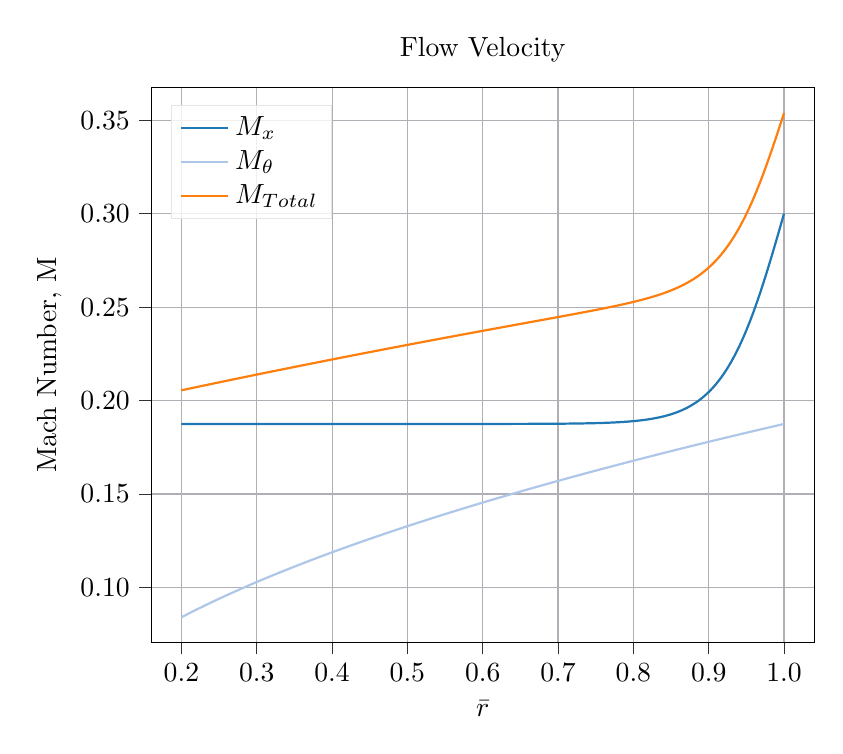
\begin{tikzpicture}

\definecolor{color0}{rgb}{0.196078431372549,0.188235294117647,0.203921568627451}
\definecolor{color1}{rgb}{0.694117647058824,0.686274509803922,0.709803921568627}
\definecolor{color2}{rgb}{0.12156862745098,0.466666666666667,0.705882352941177}
\definecolor{color3}{rgb}{0.682352941176471,0.780392156862745,0.909803921568627}
\definecolor{color4}{rgb}{1,0.498039215686275,0.0549019607843137}

\begin{axis}[
legend cell align={left},
legend style={
  fill opacity=0.8,
  draw opacity=1,
  text opacity=1,
  at={(0.03,0.97)},
  anchor=north west,
  draw=white!90!black
},
tick align=outside,
tick pos=left,
title={Flow Velocity},
width=10cm,
x grid style={color1},
xlabel={\(\displaystyle \bar{r}\)},
xmajorgrids,
xmin=0.16, xmax=1.04,
xtick style={color=color0},
xtick={0.1,0.2,0.3,0.4,0.5,0.6,0.7,0.8,0.9,1,1.1},
xticklabels={
  \(\displaystyle {0.1}\),
  \(\displaystyle {0.2}\),
  \(\displaystyle {0.3}\),
  \(\displaystyle {0.4}\),
  \(\displaystyle {0.5}\),
  \(\displaystyle {0.6}\),
  \(\displaystyle {0.7}\),
  \(\displaystyle {0.8}\),
  \(\displaystyle {0.9}\),
  \(\displaystyle {1.0}\),
  \(\displaystyle {1.1}\)
},
y grid style={color1},
ylabel={Mach Number, M},
ymajorgrids,
ymin=0.070603396545207, ymax=0.367256452050722,
ytick style={color=color0},
ytick={0.05,0.1,0.15,0.2,0.25,0.3,0.35,0.4},
yticklabels={
  \(\displaystyle {0.05}\),
  \(\displaystyle {0.10}\),
  \(\displaystyle {0.15}\),
  \(\displaystyle {0.20}\),
  \(\displaystyle {0.25}\),
  \(\displaystyle {0.30}\),
  \(\displaystyle {0.35}\),
  \(\displaystyle {0.40}\)
}
]
\addplot [thick, color2]
table {%
0.2 0.18750000046376
0.2015625 0.187500000482234
0.203125 0.187500000501444
0.2046875 0.187500000521419
0.20625 0.18750000054219
0.2078125 0.187500000563788
0.209375 0.187500000586247
0.2109375 0.1875000006096
0.2125 0.187500000633884
0.2140625 0.187500000659135
0.215625 0.187500000685392
0.2171875 0.187500000712695
0.21875 0.187500000741086
0.2203125 0.187500000770607
0.221875 0.187500000801305
0.2234375 0.187500000833225
0.225 0.187500000866417
0.2265625 0.187500000900931
0.228125 0.18750000093682
0.2296875 0.187500000974139
0.23125 0.187500001012944
0.2328125 0.187500001053295
0.234375 0.187500001095254
0.2359375 0.187500001138883
0.2375 0.187500001184252
0.2390625 0.187500001231427
0.240625 0.187500001280481
0.2421875 0.18750000133149
0.24375 0.18750000138453
0.2453125 0.187500001439684
0.246875 0.187500001497034
0.2484375 0.187500001556669
0.25 0.18750000161868
0.2515625 0.187500001683161
0.253125 0.18750000175021
0.2546875 0.187500001819931
0.25625 0.187500001892428
0.2578125 0.187500001967814
0.259375 0.187500002046203
0.2609375 0.187500002127715
0.2625 0.187500002212473
0.2640625 0.187500002300608
0.265625 0.187500002392254
0.2671875 0.18750000248755
0.26875 0.187500002586643
0.2703125 0.187500002689683
0.271875 0.187500002796828
0.2734375 0.187500002908241
0.275 0.187500003024092
0.2765625 0.187500003144558
0.278125 0.187500003269823
0.2796875 0.187500003400078
0.28125 0.187500003535522
0.2828125 0.187500003676361
0.284375 0.187500003822811
0.2859375 0.187500003975094
0.2875 0.187500004133444
0.2890625 0.187500004298102
0.290625 0.187500004469318
0.2921875 0.187500004647356
0.29375 0.187500004832485
0.2953125 0.18750000502499
0.296875 0.187500005225163
0.2984375 0.187500005433309
0.3 0.187500005649748
0.3015625 0.187500005874808
0.303125 0.187500006108834
0.3046875 0.187500006352182
0.30625 0.187500006605225
0.3078125 0.187500006868347
0.309375 0.187500007141951
0.3109375 0.187500007426454
0.3125 0.18750000772229
0.3140625 0.187500008029911
0.315625 0.187500008349786
0.3171875 0.187500008682404
0.31875 0.187500009028271
0.3203125 0.187500009387917
0.321875 0.187500009761889
0.3234375 0.187500010150758
0.325 0.187500010555119
0.3265625 0.187500010975587
0.328125 0.187500011412804
0.3296875 0.187500011867439
0.33125 0.187500012340184
0.3328125 0.187500012831761
0.334375 0.18750001334292
0.3359375 0.187500013874441
0.3375 0.187500014427136
0.3390625 0.187500015001848
0.340625 0.187500015599454
0.3421875 0.187500016220865
0.34375 0.187500016867031
0.3453125 0.187500017538937
0.346875 0.187500018237609
0.3484375 0.187500018964112
0.35 0.187500019719557
0.3515625 0.187500020505095
0.353125 0.187500021321925
0.3546875 0.187500022171293
0.35625 0.187500023054497
0.3578125 0.187500023972884
0.359375 0.187500024927855
0.3609375 0.187500025920868
0.3625 0.187500026953437
0.3640625 0.18750002802714
0.365625 0.187500029143614
0.3671875 0.187500030304564
0.36875 0.18750003151176
0.3703125 0.187500032767046
0.371875 0.187500034072337
0.3734375 0.187500035429624
0.375 0.187500036840979
0.3765625 0.187500038308557
0.378125 0.187500039834596
0.3796875 0.187500041421426
0.38125 0.187500043071467
0.3828125 0.187500044787239
0.384375 0.18750004657136
0.3859375 0.187500048426551
0.3875 0.187500050355645
0.3890625 0.187500052361586
0.390625 0.187500054447434
0.3921875 0.187500056616372
0.39375 0.187500058871712
0.3953125 0.187500061216893
0.396875 0.187500063655497
0.3984375 0.187500066191242
0.4 0.187500068828001
0.4015625 0.187500071569796
0.403125 0.187500074420812
0.4046875 0.187500077385399
0.40625 0.187500080468081
0.4078125 0.187500083673564
0.409375 0.187500087006739
0.4109375 0.187500090472692
0.4125 0.187500094076713
0.4140625 0.187500097824301
0.415625 0.187500101721177
0.4171875 0.187500105773286
0.41875 0.187500109986812
0.4203125 0.187500114368187
0.421875 0.187500118924095
0.4234375 0.18750012366149
0.425 0.187500128587601
0.4265625 0.187500133709945
0.428125 0.187500139036341
0.4296875 0.187500144574915
0.43125 0.187500150334121
0.4328125 0.187500156322748
0.434375 0.187500162549934
0.4359375 0.187500169025182
0.4375 0.187500175758374
0.4390625 0.187500182759786
0.440625 0.187500190040102
0.4421875 0.187500197610433
0.44375 0.18750020548233
0.4453125 0.187500213667808
0.446875 0.187500222179357
0.4484375 0.187500231029968
0.45 0.187500240233146
0.4515625 0.187500249802936
0.453125 0.187500259753942
0.4546875 0.18750027010135
0.45625 0.187500280860951
0.4578125 0.187500292049165
0.459375 0.187500303683066
0.4609375 0.187500315780407
0.4625 0.18750032835965
0.4640625 0.187500341439991
0.465625 0.187500355041393
0.4671875 0.187500369184611
0.46875 0.187500383891229
0.4703125 0.18750039918369
0.471875 0.187500415085331
0.4734375 0.187500431620419
0.475 0.187500448814187
0.4765625 0.187500466692875
0.478125 0.187500485283765
0.4796875 0.18750050461523
0.48125 0.187500524716768
0.4828125 0.187500545619057
0.484375 0.187500567353995
0.4859375 0.187500589954749
0.4875 0.187500613455811
0.4890625 0.187500637893043
0.490625 0.187500663303738
0.4921875 0.187500689726674
0.49375 0.187500717202174
0.4953125 0.187500745772166
0.496875 0.187500775480249
0.4984375 0.18750080637176
0.5 0.187500838493839
0.5015625 0.187500871895507
0.503125 0.187500906627735
0.5046875 0.187500942743527
0.50625 0.187500980297996
0.5078125 0.187501019348452
0.509375 0.187501059954487
0.5109375 0.187501102178067
0.5125 0.187501146083626
0.5140625 0.187501191738165
0.515625 0.187501239211355
0.5171875 0.187501288575641
0.51875 0.187501339906353
0.5203125 0.187501393281824
0.521875 0.187501448783505
0.5234375 0.187501506496092
0.525 0.187501566507656
0.5265625 0.187501628909775
0.528125 0.187501693797676
0.5296875 0.187501761270376
0.53125 0.187501831430841
0.5328125 0.187501904386134
0.534375 0.187501980247585
0.5359375 0.187502059130959
0.5375 0.187502141156631
0.5390625 0.187502226449771
0.540625 0.187502315140534
0.5421875 0.187502407364262
0.54375 0.187502503261685
0.5453125 0.18750260297914
0.546875 0.187502706668794
0.5484375 0.187502814488872
0.55 0.187502926603905
0.5515625 0.187503043184974
0.553125 0.187503164409977
0.5546875 0.187503290463896
0.55625 0.187503421539083
0.5578125 0.18750355783555
0.559375 0.187503699561276
0.5609375 0.187503846932523
0.5625 0.187504000174169
0.5640625 0.187504159520047
0.565625 0.187504325213303
0.5671875 0.18750449750677
0.56875 0.187504676663348
0.5703125 0.18750486295641
0.571875 0.187505056670217
0.5734375 0.187505258100351
0.575 0.187505467554167
0.5765625 0.187505685351261
0.578125 0.187505911823958
0.5796875 0.187506147317817
0.58125 0.187506392192163
0.5828125 0.187506646820628
0.584375 0.187506911591727
0.5859375 0.187507186909447
0.5875 0.187507473193863
0.5890625 0.187507770881781
0.590625 0.187508080427403
0.5921875 0.187508402303017
0.59375 0.18750873699972
0.5953125 0.187509085028169
0.596875 0.187509446919353
0.5984375 0.187509823225409
0.6 0.187510214520458
0.6015625 0.187510621401487
0.603125 0.187511044489252
0.6046875 0.187511484429231
0.60625 0.187511941892601
0.6078125 0.187512417577267
0.609375 0.187512912208923
0.6109375 0.187513426542158
0.6125 0.187513961361605
0.6140625 0.187514517483141
0.615625 0.187515095755124
0.6171875 0.187515697059692
0.61875 0.187516322314102
0.6203125 0.18751697247213
0.621875 0.187517648525525
0.6234375 0.187518351505516
0.625 0.187519082484388
0.6265625 0.18751984257711
0.628125 0.187520632943037
0.6296875 0.187521454787673
0.63125 0.187522309364511
0.6328125 0.187523197976934
0.634375 0.187524121980207
0.6359375 0.187525082783537
0.6375 0.187526081852217
0.6390625 0.187527120709858
0.640625 0.187528200940708
0.6421875 0.187529324192061
0.64375 0.187530492176765
0.6453125 0.187531706675829
0.646875 0.187532969541129
0.6484375 0.187534282698227
0.65 0.187535648149298
0.6515625 0.187537067976177
0.653125 0.187538544343523
0.6546875 0.187540079502106
0.65625 0.187541675792235
0.6578125 0.187543335647307
0.659375 0.187545061597511
0.6609375 0.187546856273668
0.6625 0.187548722411226
0.6640625 0.187550662854418
0.665625 0.187552680560575
0.6671875 0.18755477860462
0.66875 0.187556960183734
0.6703125 0.187559228622203
0.671875 0.187561587376466
0.6734375 0.187564040040354
0.675 0.18756659035054
0.6765625 0.187569242192204
0.678125 0.187571999604917
0.6796875 0.187574866788767
0.68125 0.187577848110715
0.6828125 0.187580948111211
0.684375 0.187584171511064
0.6859375 0.187587523218585
0.6875 0.187591008337014
0.6890625 0.187594632172234
0.690625 0.187598400240792
0.6921875 0.187602318278233
0.69375 0.187606392247767
0.6953125 0.187610628349266
0.696875 0.187615033028623
0.6984375 0.187619612987475
0.7 0.187624375193308
0.7015625 0.187629326889952
0.703125 0.187634475608498
0.7046875 0.187639829178631
0.70625 0.187645395740412
0.7078125 0.187651183756517
0.709375 0.187657202024959
0.7109375 0.187663459692296
0.7125 0.187669966267364
0.7140625 0.187676731635538
0.715625 0.18768376607355
0.7171875 0.187691080264881
0.71875 0.187698685315752
0.7203125 0.187706592771732
0.721875 0.187714814634993
0.7234375 0.18772336338223
0.725 0.18773225198327
0.7265625 0.187741493920405
0.728125 0.187751103208465
0.7296875 0.187761094415665
0.73125 0.187771482685255
0.7328125 0.187782283757994
0.734375 0.187793513995488
0.7359375 0.187805190404429
0.7375 0.187817330661739
0.7390625 0.187829953140694
0.740625 0.187843076938026
0.7421875 0.18785672190206
0.74375 0.187870908661916
0.7453125 0.187885658657817
0.746875 0.187900994172532
0.7484375 0.187916938364013
0.75 0.187933515299249
0.7515625 0.18795074998939
0.753125 0.187968668426185
0.7546875 0.187987297619776
0.75625 0.188006665637888
0.7578125 0.188026801646486
0.759375 0.188047735951914
0.7609375 0.188069500044599
0.7625 0.188092126644349
0.7640625 0.188115649747308
0.765625 0.18814010467462
0.7671875 0.188165528122856
0.76875 0.188191958216261
0.7703125 0.18821943456088
0.771875 0.188247998300622
0.7734375 0.188277692175315
0.775 0.188308560580819
0.7765625 0.188340649631268
0.778125 0.188374007223472
0.7796875 0.188408683103589
0.78125 0.188444728936081
0.7828125 0.188482198375064
0.784375 0.188521147138079
0.7859375 0.188561633082381
0.7875 0.188603716283787
0.7890625 0.188647459118164
0.790625 0.188692926345615
0.7921875 0.188740185197431
0.79375 0.188789305465873
0.7953125 0.188840359596844
0.796875 0.188893422785517
0.7984375 0.188948573074984
0.8 0.189005891457964
0.8015625 0.18906546198166
0.803125 0.189127371855783
0.8046875 0.189191711563822
0.80625 0.18925857497759
0.8078125 0.189328059475091
0.809375 0.189400266061753
0.8109375 0.189475299495055
0.8125 0.189553268412566
0.8140625 0.189634285463429
0.815625 0.189718467443296
0.8171875 0.189805935432711
0.81875 0.189896814938938
0.8203125 0.189991236041228
0.821875 0.190089333539468
0.8234375 0.190191247106207
0.825 0.190297121441967
0.8265625 0.190407106433793
0.828125 0.190521357316943
0.8296875 0.190640034839612
0.83125 0.190763305430561
0.8328125 0.190891341369513
0.834375 0.191024320960125
0.8359375 0.19116242870536
0.8375 0.191305855485013
0.8390625 0.191454798735151
0.840625 0.191609462629168
0.8421875 0.191770058260147
0.84375 0.191936803824153
0.8453125 0.192109924804067
0.846875 0.192289654153526
0.8484375 0.192476232480468
0.85 0.192669908229756
0.8515625 0.192870937864297
0.853125 0.193079586044007
0.8546875 0.193296125801925
0.85625 0.193520838716725
0.8578125 0.19375401508078
0.859375 0.193995954062915
0.8609375 0.19424696386485
0.8625 0.194507361870325
0.8640625 0.19477747478576
0.865625 0.195057638771273
0.8671875 0.195348199560753
0.86875 0.195649512569619
0.8703125 0.195961942988806
0.871875 0.196285865863401
0.8734375 0.196621666154283
0.875 0.196969738781014
0.8765625 0.197330488644105
0.878125 0.197704330624719
0.8796875 0.19809168955973
0.88125 0.198493000189989
0.8828125 0.198908707079512
0.884375 0.199339264503236
0.8859375 0.199785136300872
0.8875 0.200246795694294
0.8890625 0.200724725065815
0.890625 0.201219415694617
0.8921875 0.201731367448532
0.89375 0.20226108842829
0.8953125 0.202809094561326
0.896875 0.203375909142141
0.8984375 0.203962062316265
0.9 0.20456809050478
0.9015625 0.205194535766423
0.903125 0.205841945094312
0.9046875 0.206510869644377
0.90625 0.207201863892688
0.9078125 0.207915484718967
0.909375 0.208652290413729
0.9109375 0.209412839606688
0.9125 0.210197690114263
0.9140625 0.211007397704303
0.915625 0.211842514776466
0.9171875 0.212703588957001
0.91875 0.213591161607143
0.9203125 0.214505766244731
0.921875 0.215447926879212
0.9234375 0.216418156260711
0.925 0.217416954044512
0.9265625 0.218444804872919
0.928125 0.219502176377227
0.9296875 0.220589517103286
0.93125 0.221707254364989
0.9328125 0.222855792030882
0.934375 0.22403550825001
0.9359375 0.225246753124095
0.9375 0.226489846334098
0.9390625 0.227765074730271
0.940625 0.2290726898958
0.9421875 0.230412905695208
0.94375 0.231785895819697
0.9453125 0.233191791342631
0.946875 0.234630678299323
0.9484375 0.236102595306257
0.95 0.237607531235694
0.9515625 0.239145422962452
0.953125 0.240716153200284
0.9546875 0.242319548445916
0.95625 0.243955377049186
0.9578125 0.245623347428067
0.959375 0.247323106447459
0.9609375 0.249054237980582
0.9625 0.250816261671558
0.9640625 0.252608631917287
0.965625 0.254430737086079
0.9671875 0.256281898989545
0.96875 0.258161372623157
0.9703125 0.260068346189484
0.971875 0.262001941416523
0.9734375 0.263961214181707
0.975 0.265945155450138
0.9765625 0.267952692533349
0.978125 0.269982690672486
0.9796875 0.272033954947202
0.98125 0.274105232508885
0.9828125 0.276195215133999
0.984375 0.278302542090459
0.9859375 0.280425803307079
0.9875 0.282563542833192
0.9890625 0.284714262572769
0.990625 0.286876426274541
0.9921875 0.289048463757075
0.99375 0.291228775345271
0.9953125 0.293415736492518
0.996875 0.295607702560779
0.9984375 0.297803013729147
1 0.3
};
\addlegendentry{$M_{x}$}
\addplot [thick, color3]
table {%
0.2 0.0840876263409123
0.2015625 0.0844149965067977
0.203125 0.0847410948951383
0.2046875 0.0850659361314183
0.20625 0.0853895345626085
0.2078125 0.085711904264537
0.209375 0.0860330590490097
0.2109375 0.086353012470694
0.2125 0.0866717778337715
0.2140625 0.0869893681983725
0.215625 0.0873057963867985
0.2171875 0.0876210749895433
0.21875 0.0879352163711182
0.2203125 0.0882482326756911
0.221875 0.0885601358325461
0.2234375 0.0888709375613698
0.225 0.0891806493773721
0.2265625 0.0894892825962467
0.228125 0.0897968483389784
0.2296875 0.0901033575365025
0.23125 0.0904088209342211
0.2328125 0.0907132490963835
0.234375 0.0910166524103334
0.2359375 0.0913190410906296
0.2375 0.091620425183044
0.2390625 0.0919208145684408
0.240625 0.0922202189665431
0.2421875 0.0925186479395882
0.24375 0.092816110895878
0.2453125 0.0931126170932264
0.246875 0.0934081756423087
0.2484375 0.0937027955099154
0.25 0.0939964855221141
0.2515625 0.0942892543673225
0.253125 0.0945811105992962
0.2546875 0.0948720626400325
0.25625 0.0951621187825959
0.2578125 0.095451287193864
0.259375 0.0957395759172009
0.2609375 0.0960269928750565
0.2625 0.0963135458714966
0.2640625 0.0965992425946655
0.265625 0.0968840906191826
0.2671875 0.0971680974084761
0.26875 0.0974512703170552
0.2703125 0.097733616592723
0.271875 0.0980151433787315
0.2734375 0.0982958577158822
0.275 0.0985757665445709
0.2765625 0.0988548767067819
0.278125 0.0991331949480311
0.2796875 0.0994107279192592
0.28125 0.0996874821786789
0.2828125 0.0999634641935747
0.284375 0.100238680342059
0.2859375 0.100513136914783
0.2875 0.100786840116609
0.2890625 0.101059796068238
0.290625 0.101332010807801
0.2921875 0.10160349029241
0.29375 0.101874240399669
0.2953125 0.102144266929159
0.296875 0.102413575603874
0.2984375 0.102682172071632
0.3 0.102950061906454
0.3015625 0.103217250609899
0.303125 0.103483743612387
0.3046875 0.10374954627447
0.30625 0.104014663888094
0.3078125 0.104279101677813
0.309375 0.104542864801993
0.3109375 0.104805958353973
0.3125 0.105068387363213
0.3140625 0.105330156796407
0.315625 0.105591271558575
0.3171875 0.105851736494131
0.31875 0.106111556387925
0.3203125 0.106370735966266
0.321875 0.106629279897915
0.3234375 0.10688719279507
0.325 0.107144479214311
0.3265625 0.107401143657541
0.328125 0.107657190572902
0.3296875 0.107912624355661
0.33125 0.108167449349096
0.3328125 0.108421669845348
0.334375 0.108675290086259
0.3359375 0.108928314264198
0.3375 0.109180746522859
0.3390625 0.109432590958057
0.340625 0.109683851618491
0.3421875 0.109934532506504
0.34375 0.110184637578823
0.3453125 0.11043417074728
0.346875 0.110683135879529
0.3484375 0.110931536799732
0.35 0.111179377289251
0.3515625 0.111426661087307
0.353125 0.111673391891641
0.3546875 0.111919573359152
0.35625 0.112165209106527
0.3578125 0.112410302710859
0.359375 0.112654857710248
0.3609375 0.112898877604396
0.3625 0.113142365855188
0.3640625 0.113385325887261
0.365625 0.113627761088564
0.3671875 0.113869674810904
0.36875 0.114111070370485
0.3703125 0.114351951048436
0.371875 0.114592320091327
0.3734375 0.114832180711677
0.375 0.115071536088453
0.3765625 0.115310389367555
0.378125 0.115548743662302
0.3796875 0.115786602053898
0.38125 0.116023967591893
0.3828125 0.116260843294641
0.384375 0.116497232149742
0.3859375 0.116733137114479
0.3875 0.116968561116248
0.3890625 0.11720350705298
0.390625 0.117437977793553
0.3921875 0.117671976178199
0.39375 0.117905505018902
0.3953125 0.118138567099792
0.396875 0.118371165177528
0.3984375 0.118603301981677
0.4 0.118834980215086
0.4015625 0.119066202554244
0.403125 0.119296971649644
0.4046875 0.119527290126133
0.40625 0.11975716058326
0.4078125 0.119986585595614
0.409375 0.12021556771316
0.4109375 0.120444109461566
0.4125 0.120672213342528
0.4140625 0.120899881834087
0.415625 0.121127117390938
0.4171875 0.121353922444742
0.41875 0.121580299404422
0.4203125 0.121806250656465
0.421875 0.12203177856521
0.4234375 0.122256885473136
0.425 0.122481573701142
0.4265625 0.122705845548829
0.428125 0.122929703294769
0.4296875 0.123153149196773
0.43125 0.123376185492156
0.4328125 0.123598814398
0.434375 0.123821038111401
0.4359375 0.124042858809731
0.4375 0.124264278650875
0.4390625 0.124485299773482
0.440625 0.124705924297198
0.4421875 0.124926154322909
0.44375 0.125145991932965
0.4453125 0.125365439191413
0.446875 0.125584498144222
0.4484375 0.125803170819498
0.45 0.12602145922771
0.4515625 0.126239365361899
0.453125 0.126456891197888
0.4546875 0.126674038694493
0.45625 0.126890809793726
0.4578125 0.127107206420994
0.459375 0.1273232304853
0.4609375 0.127538883879439
0.4625 0.127754168480184
0.4640625 0.127969086148483
0.465625 0.128183638729641
0.4671875 0.128397828053503
0.46875 0.128611655934637
0.4703125 0.128825124172511
0.471875 0.129038234551667
0.4734375 0.129250988841897
0.475 0.129463388798411
0.4765625 0.129675436162004
0.478125 0.129887132659225
0.4796875 0.130098480002534
0.48125 0.130309479890467
0.4828125 0.130520134007792
0.484375 0.130730444025667
0.4859375 0.130940411601791
0.4875 0.131150038380555
0.4890625 0.131359325993194
0.490625 0.131568276057931
0.4921875 0.131776890180125
0.49375 0.131985169952409
0.4953125 0.132193116954838
0.496875 0.132400732755019
0.4984375 0.132608018908254
0.5 0.132814976957676
0.5015625 0.133021608434374
0.503125 0.133227914857534
0.5046875 0.133433897734562
0.50625 0.133639558561211
0.5078125 0.133844898821711
0.509375 0.134049919988891
0.5109375 0.134254623524301
0.5125 0.134459010878331
0.5140625 0.134663083490334
0.515625 0.134866842788739
0.5171875 0.13507029019117
0.51875 0.135273427104558
0.5203125 0.135476254925255
0.521875 0.135678775039143
0.5234375 0.135880988821749
0.525 0.136082897638344
0.5265625 0.136284502844058
0.528125 0.136485805783982
0.5296875 0.136686807793271
0.53125 0.136887510197249
0.5328125 0.137087914311505
0.534375 0.137288021442002
0.5359375 0.137487832885164
0.5375 0.137687349927982
0.5390625 0.137886573848107
0.540625 0.138085505913944
0.5421875 0.138284147384745
0.54375 0.138482499510704
0.5453125 0.138680563533045
0.546875 0.138878340684114
0.5484375 0.139075832187464
0.55 0.13927303925795
0.5515625 0.139469963101806
0.553125 0.139666604916739
0.5546875 0.139862965892007
0.55625 0.140059047208505
0.5578125 0.140254850038847
0.559375 0.140450375547447
0.5609375 0.140645624890599
0.5625 0.140840599216554
0.5640625 0.141035299665604
0.565625 0.141229727370151
0.5671875 0.141423883454791
0.56875 0.141617769036382
0.5703125 0.141811385224125
0.571875 0.142004733119633
0.5734375 0.142197813817004
0.575 0.142390628402895
0.5765625 0.14258317795659
0.578125 0.142775463550071
0.5796875 0.142967486248087
0.58125 0.143159247108222
0.5828125 0.143350747180962
0.584375 0.143541987509764
0.5859375 0.143732969131117
0.5875 0.143923693074612
0.5890625 0.144114160363001
0.590625 0.144304372012265
0.5921875 0.144494329031676
0.59375 0.144684032423856
0.5953125 0.144873483184839
0.596875 0.145062682304136
0.5984375 0.145251630764788
0.6 0.145440329543428
0.6015625 0.145628779610342
0.603125 0.145816981929523
0.6046875 0.146004937458728
0.60625 0.146192647149536
0.6078125 0.146380111947405
0.609375 0.146567332791723
0.6109375 0.146754310615866
0.6125 0.14694104634725
0.6140625 0.147127540907384
0.615625 0.147313795211923
0.6171875 0.147499810170722
0.61875 0.147685586687883
0.6203125 0.14787112566181
0.621875 0.148056427985255
0.6234375 0.148241494545374
0.625 0.148426326223768
0.6265625 0.148610923896538
0.628125 0.148795288434329
0.6296875 0.148979420702382
0.63125 0.149163321560575
0.6328125 0.149346991863473
0.634375 0.149530432460373
0.6359375 0.149713644195352
0.6375 0.149896627907306
0.6390625 0.150079384430001
0.640625 0.15026191459211
0.6421875 0.150444219217264
0.64375 0.150626299124089
0.6453125 0.150808155126251
0.646875 0.150989788032497
0.6484375 0.151171198646697
0.65 0.151352387767887
0.6515625 0.151533356190305
0.653125 0.151714104703435
0.6546875 0.151894634092048
0.65625 0.152074945136236
0.6578125 0.152255038611455
0.659375 0.152434915288563
0.6609375 0.152614575933858
0.6625 0.152794021309115
0.6640625 0.152973252171623
0.665625 0.153152269274223
0.6671875 0.153331073365345
0.66875 0.153509665189041
0.6703125 0.153688045485025
0.671875 0.153866214988707
0.6734375 0.154044174431223
0.675 0.15422192453948
0.6765625 0.15439946603618
0.678125 0.154576799639858
0.6796875 0.15475392606492
0.68125 0.154930846021666
0.6828125 0.155107560216335
0.684375 0.155284069351125
0.6859375 0.155460374124238
0.6875 0.155636475229901
0.6890625 0.155812373358403
0.690625 0.155988069196127
0.6921875 0.156163563425576
0.69375 0.156338856725411
0.6953125 0.156513949770474
0.696875 0.15668884323182
0.6984375 0.156863537776752
0.7 0.157038034068843
0.7015625 0.157212332767968
0.703125 0.157386434530335
0.7046875 0.15756034000851
0.70625 0.157734049851447
0.7078125 0.157907564704515
0.709375 0.158080885209529
0.7109375 0.158254012004772
0.7125 0.158426945725027
0.7140625 0.158599687001598
0.715625 0.158772236462346
0.7171875 0.158944594731704
0.71875 0.159116762430712
0.7203125 0.159288740177039
0.721875 0.159460528585009
0.7234375 0.159632128265627
0.725 0.159803539826601
0.7265625 0.159974763872372
0.728125 0.160145801004136
0.7296875 0.160316651819865
0.73125 0.160487316914339
0.7328125 0.160657796879161
0.734375 0.160828092302788
0.7359375 0.160998203770549
0.7375 0.161168131864673
0.7390625 0.161337877164308
0.740625 0.161507440245544
0.7421875 0.16167682168144
0.74375 0.16184602204204
0.7453125 0.162015041894401
0.746875 0.162183881802611
0.7484375 0.162352542327811
0.75 0.162521024028219
0.7515625 0.162689327459149
0.753125 0.162857453173033
0.7546875 0.163025401719442
0.75625 0.163193173645105
0.7578125 0.163360769493934
0.759375 0.163528189807038
0.7609375 0.163695435122748
0.7625 0.163862505976635
0.7640625 0.164029402901533
0.765625 0.16419612642755
0.7671875 0.164362677082099
0.76875 0.164529055389908
0.7703125 0.164695261873044
0.771875 0.164861297050929
0.7734375 0.165027161440362
0.775 0.165192855555533
0.7765625 0.165358379908047
0.778125 0.165523735006937
0.7796875 0.165688921358686
0.78125 0.165853939467241
0.7828125 0.166018789834035
0.784375 0.166183472958
0.7859375 0.16634798933559
0.7875 0.166512339460793
0.7890625 0.166676523825149
0.790625 0.166840542917772
0.7921875 0.167004397225359
0.79375 0.167168087232212
0.7953125 0.167331613420254
0.796875 0.167494976269043
0.7984375 0.16765817625579
0.8 0.167821213855375
0.8015625 0.167984089540363
0.803125 0.168146803781017
0.8046875 0.168309357045319
0.80625 0.168471749798981
0.8078125 0.168633982505463
0.809375 0.168796055625984
0.8109375 0.168957969619545
0.8125 0.169119724942935
0.8140625 0.169281322050753
0.815625 0.169442761395417
0.8171875 0.169604043427185
0.81875 0.169765168594161
0.8203125 0.16992613734232
0.821875 0.170086950115511
0.8234375 0.170247607355479
0.825 0.170408109501878
0.8265625 0.170568456992279
0.828125 0.170728650262193
0.8296875 0.170888689745076
0.83125 0.171048575872349
0.8328125 0.171208309073405
0.834375 0.171367889775629
0.8359375 0.171527318404407
0.8375 0.171686595383141
0.8390625 0.171845721133259
0.840625 0.172004696074232
0.8421875 0.172163520623583
0.84375 0.172322195196902
0.8453125 0.172480720207858
0.846875 0.172639096068211
0.8484375 0.172797323187825
0.85 0.172955401974678
0.8515625 0.173113332834877
0.853125 0.17327111617267
0.8546875 0.173428752390454
0.85625 0.173586241888793
0.8578125 0.173743585066423
0.859375 0.173900782320269
0.8609375 0.174057834045453
0.8625 0.174214740635309
0.8640625 0.174371502481389
0.865625 0.174528119973481
0.8671875 0.174684593499615
0.86875 0.174840923446074
0.8703125 0.17499711019741
0.871875 0.175153154136449
0.8734375 0.175309055644305
0.875 0.17546481510039
0.8765625 0.175620432882426
0.878125 0.175775909366452
0.8796875 0.175931244926839
0.88125 0.176086439936296
0.8828125 0.176241494765883
0.884375 0.176396409785022
0.8859375 0.176551185361503
0.8875 0.176705821861499
0.8890625 0.176860319649574
0.890625 0.177014679088689
0.8921875 0.17716890054022
0.89375 0.17732298436396
0.8953125 0.177476930918133
0.896875 0.177630740559403
0.8984375 0.177784413642882
0.9 0.17793795052214
0.9015625 0.178091351549215
0.903125 0.178244617074622
0.9046875 0.178397747447363
0.90625 0.178550743014934
0.9078125 0.178703604123336
0.909375 0.178856331117085
0.9109375 0.179008924339215
0.9125 0.179161384131296
0.9140625 0.179313710833435
0.915625 0.179465904784289
0.9171875 0.179617966321072
0.91875 0.179769895779564
0.9203125 0.179921693494119
0.921875 0.180073359797674
0.9234375 0.180224895021759
0.925 0.180376299496502
0.9265625 0.18052757355064
0.928125 0.180678717511524
0.9296875 0.180829731705132
0.93125 0.180980616456073
0.9328125 0.181131372087597
0.934375 0.181281998921602
0.9359375 0.181432497278642
0.9375 0.181582867477936
0.9390625 0.181733109837375
0.940625 0.181883224673528
0.9421875 0.182033212301652
0.94375 0.182183073035701
0.9453125 0.18233280718833
0.946875 0.182482415070901
0.9484375 0.182631896993499
0.95 0.182781253264931
0.9515625 0.182930484192734
0.953125 0.183079590083189
0.9546875 0.18322857124132
0.95625 0.183377427970906
0.9578125 0.183526160574488
0.959375 0.183674769353373
0.9609375 0.183823254607646
0.9625 0.18397161663617
0.9640625 0.184119855736599
0.965625 0.184267972205384
0.9671875 0.184415966337778
0.96875 0.184563838427841
0.9703125 0.184711588768452
0.971875 0.18485921765131
0.9734375 0.185006725366947
0.975 0.185154112204728
0.9765625 0.18530137845286
0.978125 0.185448524398402
0.9796875 0.185595550327265
0.98125 0.185742456524225
0.9828125 0.185889243272923
0.984375 0.186035910855876
0.9859375 0.186182459554481
0.9875 0.186328889649023
0.9890625 0.186475201418678
0.990625 0.186621395141524
0.9921875 0.18676747109454
0.99375 0.18691342955362
0.9953125 0.187059270793574
0.996875 0.187204995088134
0.9984375 0.187350602709962
1 0.187496093930656
};
\addlegendentry{$M_{\theta}$}
\addplot [thick, color4]
table {%
0.2 0.205492041397127
0.2015625 0.205626218698103
0.203125 0.205760305579254
0.2046875 0.205894302217052
0.20625 0.206028208787389
0.2078125 0.206162025465588
0.209375 0.206295752426396
0.2109375 0.206429389843995
0.2125 0.206562937891997
0.2140625 0.206696396743455
0.215625 0.206829766570857
0.2171875 0.206963047546135
0.21875 0.207096239840666
0.2203125 0.207229343625271
0.221875 0.207362359070223
0.2234375 0.207495286345247
0.225 0.207628125619522
0.2265625 0.207760877061684
0.228125 0.207893540839827
0.2296875 0.208026117121511
0.23125 0.208158606073758
0.2328125 0.208291007863057
0.234375 0.208423322655368
0.2359375 0.208555550616121
0.2375 0.208687691910223
0.2390625 0.208819746702056
0.240625 0.208951715155482
0.2421875 0.209083597433845
0.24375 0.209215393699973
0.2453125 0.209347104116181
0.246875 0.209478728844272
0.2484375 0.209610268045542
0.25 0.209741721880779
0.2515625 0.209873090510267
0.253125 0.210004374093791
0.2546875 0.210135572790635
0.25625 0.210266686759585
0.2578125 0.210397716158935
0.259375 0.210528661146485
0.2609375 0.210659521879546
0.2625 0.210790298514942
0.2640625 0.210920991209009
0.265625 0.211051600117604
0.2671875 0.211182125396101
0.26875 0.211312567199395
0.2703125 0.211442925681907
0.271875 0.211573200997583
0.2734375 0.211703393299898
0.275 0.211833502741857
0.2765625 0.211963529475998
0.278125 0.212093473654396
0.2796875 0.212223335428662
0.28125 0.212353114949946
0.2828125 0.212482812368943
0.284375 0.21261242783589
0.2859375 0.21274196150057
0.2875 0.212871413512318
0.2890625 0.213000784020017
0.290625 0.213130073172105
0.2921875 0.213259281116575
0.29375 0.213388408000978
0.2953125 0.213517453972425
0.296875 0.21364641917759
0.2984375 0.213775303762711
0.3 0.213904107873594
0.3015625 0.214032831655613
0.303125 0.214161475253714
0.3046875 0.214290038812416
0.30625 0.214418522475817
0.3078125 0.21454692638759
0.309375 0.21467525069099
0.3109375 0.214803495528855
0.3125 0.214931661043609
0.3140625 0.215059747377263
0.315625 0.215187754671418
0.3171875 0.215315683067268
0.31875 0.215443532705602
0.3203125 0.215571303726804
0.321875 0.21569899627086
0.3234375 0.215826610477357
0.325 0.215954146485487
0.3265625 0.216081604434049
0.328125 0.216208984461451
0.3296875 0.216336286705711
0.33125 0.216463511304465
0.3328125 0.216590658394964
0.334375 0.216717728114079
0.3359375 0.216844720598302
0.3375 0.216971635983751
0.3390625 0.21709847440617
0.340625 0.217225236000936
0.3421875 0.217351920903056
0.34375 0.217478529247173
0.3453125 0.217605061167568
0.346875 0.217731516798165
0.3484375 0.217857896272531
0.35 0.217984199723878
0.3515625 0.218110427285071
0.353125 0.218236579088626
0.3546875 0.218362655266715
0.35625 0.218488655951168
0.3578125 0.21861458127348
0.359375 0.218740431364808
0.3609375 0.21886620635598
0.3625 0.218991906377494
0.3640625 0.219117531559524
0.365625 0.219243082031922
0.3671875 0.219368557924223
0.36875 0.219493959365648
0.3703125 0.219619286485106
0.371875 0.2197445394112
0.3734375 0.219869718272229
0.375 0.219994823196194
0.3765625 0.220119854310799
0.378125 0.220244811743459
0.3796875 0.220369695621299
0.38125 0.220494506071164
0.3828125 0.22061924321962
0.384375 0.220743907192957
0.3859375 0.220868498117198
0.3875 0.220993016118101
0.3890625 0.221117461321162
0.390625 0.221241833851624
0.3921875 0.221366133834481
0.39375 0.22149036139448
0.3953125 0.221614516656131
0.396875 0.221738599743709
0.3984375 0.221862610781261
0.4 0.221986549892612
0.4015625 0.222110417201371
0.403125 0.222234212830936
0.4046875 0.222357936904504
0.40625 0.222481589545072
0.4078125 0.222605170875447
0.409375 0.222728681018256
0.4109375 0.222852120095945
0.4125 0.222975488230794
0.4140625 0.223098785544921
0.415625 0.223222012160292
0.4171875 0.223345168198727
0.41875 0.223468253781909
0.4203125 0.223591269031393
0.421875 0.223714214068615
0.4234375 0.223837089014902
0.425 0.22395989399148
0.4265625 0.224082629119485
0.428125 0.224205294519971
0.4296875 0.224327890313926
0.43125 0.224450416622275
0.4328125 0.224572873565901
0.434375 0.224695261265645
0.4359375 0.22481757984233
0.4375 0.224939829416766
0.4390625 0.225062010109763
0.440625 0.225184122042148
0.4421875 0.225306165334779
0.44375 0.225428140108554
0.4453125 0.225550046484432
0.446875 0.225671884583447
0.4484375 0.225793654526719
0.45 0.225915356435477
0.4515625 0.226036990431076
0.453125 0.226158556635008
0.4546875 0.226280055168928
0.45625 0.22640148615467
0.4578125 0.226522849714265
0.459375 0.226644145969965
0.4609375 0.226765375044263
0.4625 0.226886537059914
0.4640625 0.22700763213996
0.465625 0.227128660407751
0.4671875 0.227249621986974
0.46875 0.227370517001672
0.4703125 0.227491345576278
0.471875 0.227612107835638
0.4734375 0.22773280390504
0.475 0.227853433910245
0.4765625 0.227973997977515
0.478125 0.22809449623365
0.4796875 0.228214928806017
0.48125 0.228335295822585
0.4828125 0.228455597411962
0.484375 0.22857583370343
0.4859375 0.228696004826988
0.4875 0.228816110913385
0.4890625 0.228936152094168
0.490625 0.229056128501723
0.4921875 0.229176040269316
0.49375 0.229295887531146
0.4953125 0.229415670422388
0.496875 0.229535389079245
0.4984375 0.229655043639002
0.5 0.229774634240076
0.5015625 0.229894161022074
0.503125 0.230013624125853
0.5046875 0.230133023693578
0.50625 0.230252359868786
0.5078125 0.23037163279645
0.509375 0.230490842623051
0.5109375 0.230609989496642
0.5125 0.230729073566927
0.5140625 0.230848094985332
0.515625 0.230967053905089
0.5171875 0.231085950481315
0.51875 0.231204784871096
0.5203125 0.231323557233581
0.521875 0.231442267730066
0.5234375 0.231560916524098
0.525 0.231679503781567
0.5265625 0.231798029670813
0.528125 0.231916494362734
0.5296875 0.232034898030895
0.53125 0.232153240851643
0.5328125 0.232271523004232
0.534375 0.232389744670942
0.5359375 0.232507906037211
0.5375 0.232626007291772
0.5390625 0.232744048626792
0.540625 0.232862030238015
0.5421875 0.232979952324915
0.54375 0.233097815090855
0.5453125 0.233215618743248
0.546875 0.233333363493729
0.5484375 0.233451049558326
0.55 0.233568677157653
0.5515625 0.233686246517088
0.553125 0.233803757866984
0.5546875 0.233921211442864
0.55625 0.23403860748564
0.5578125 0.234155946241835
0.559375 0.234273227963812
0.5609375 0.234390452910015
0.5625 0.23450762134522
0.5640625 0.234624733540788
0.565625 0.234741789774943
0.5671875 0.234858790333043
0.56875 0.234975735507879
0.5703125 0.235092625599969
0.571875 0.235209460917879
0.5734375 0.235326241778546
0.575 0.235442968507616
0.5765625 0.235559641439799
0.578125 0.235676260919235
0.5796875 0.235792827299873
0.58125 0.235909340945869
0.5828125 0.236025802231993
0.584375 0.236142211544063
0.5859375 0.236258569279383
0.5875 0.236374875847207
0.5890625 0.236491131669218
0.590625 0.236607337180028
0.5921875 0.236723492827696
0.59375 0.236839599074263
0.5953125 0.236955656396316
0.596875 0.237071665285568
0.5984375 0.237187626249461
0.6 0.237303539811797
0.6015625 0.237419406513388
0.603125 0.237535226912736
0.6046875 0.23765100158674
0.60625 0.237766731131424
0.6078125 0.237882416162705
0.609375 0.237998057317179
0.6109375 0.238113655252947
0.6125 0.23822921065047
0.6140625 0.238344724213457
0.615625 0.238460196669788
0.6171875 0.238575628772474
0.61875 0.238691021300656
0.6203125 0.238806375060643
0.621875 0.238921690886984
0.6234375 0.239036969643594
0.625 0.239152212224915
0.6265625 0.239267419557128
0.628125 0.239382592599404
0.6296875 0.23949773234522
0.63125 0.23961283982371
0.6328125 0.239727916101076
0.634375 0.239842962282061
0.6359375 0.239957979511466
0.6375 0.240072968975738
0.6390625 0.240187931904618
0.640625 0.240302869572848
0.6421875 0.24041778330195
0.64375 0.240532674462077
0.6453125 0.240647544473931
0.646875 0.24076239481076
0.6484375 0.240877227000432
0.65 0.24099204262759
0.6515625 0.241106843335894
0.653125 0.241221630830348
0.6546875 0.241336406879719
0.65625 0.241451173319056
0.6578125 0.241565932052295
0.659375 0.241680685054983
0.6609375 0.241795434377094
0.6625 0.241910182145964
0.6640625 0.242024930569341
0.665625 0.242139681938548
0.6671875 0.242254438631776
0.66875 0.242369203117505
0.6703125 0.242483977958056
0.671875 0.242598765813288
0.6734375 0.242713569444431
0.675 0.242828391718078
0.6765625 0.242943235610327
0.678125 0.243058104211087
0.6796875 0.243173000728556
0.68125 0.243287928493865
0.6828125 0.243402890965914
0.684375 0.243517891736393
0.6859375 0.243632934534991
0.6875 0.243748023234826
0.6890625 0.243863161858068
0.690625 0.243978354581794
0.6921875 0.24409360574407
0.69375 0.244208919850262
0.6953125 0.244324301579603
0.696875 0.244439755792009
0.6984375 0.244555287535168
0.7 0.244670902051891
0.7015625 0.244786604787768
0.703125 0.244902401399103
0.7046875 0.245018297761173
0.70625 0.245134299976797
0.7078125 0.245250414385242
0.709375 0.245366647571476
0.7109375 0.245483006375775
0.7125 0.245599497903709
0.7140625 0.24571612953651
0.715625 0.245832908941838
0.7171875 0.245949844084975
0.71875 0.246066943240438
0.7203125 0.246184215004051
0.721875 0.246301668305475
0.7234375 0.246419312421227
0.725 0.246537156988195
0.7265625 0.24665521201768
0.728125 0.246773487909969
0.7296875 0.246891995469477
0.73125 0.247010745920461
0.7328125 0.247129750923343
0.734375 0.247249022591653
0.7359375 0.247368573509626
0.7375 0.247488416750461
0.7390625 0.247608565895287
0.740625 0.247729035052844
0.7421875 0.247849838879915
0.74375 0.247970992602536
0.7453125 0.248092512038003
0.746875 0.248214413617722
0.7484375 0.248336714410914
0.75 0.248459432149222
0.7515625 0.248582585252234
0.753125 0.248706192853978
0.7546875 0.248830274830398
0.75625 0.248954851827873
0.7578125 0.249079945292785
0.759375 0.249205577502204
0.7609375 0.249331771595701
0.7625 0.249458551608352
0.7640625 0.249585942504952
0.765625 0.249713970215503
0.7671875 0.249842661671997
0.76875 0.249972044846552
0.7703125 0.250102148790945
0.771875 0.250233003677584
0.7734375 0.250364640841964
0.775 0.250497092826666
0.7765625 0.250630393426938
0.778125 0.250764577737916
0.7796875 0.250899682203532
0.78125 0.251035744667161
0.7828125 0.251172804424074
0.784375 0.251310902275726
0.7859375 0.251450080585965
0.7875 0.251590383339192
0.7890625 0.251731856200551
0.790625 0.25187454657819
0.7921875 0.252018503687658
0.79375 0.252163778618507
0.7953125 0.252310424403136
0.796875 0.252458496087962
0.7984375 0.252608050806957
0.8 0.252759147857622
0.8015625 0.252911848779457
0.803125 0.253066217434978
0.8046875 0.253222320093347
0.80625 0.25338022551667
0.8078125 0.253540005049018
0.809375 0.253701732708221
0.8109375 0.253865485280493
0.8125 0.254031342417939
0.8140625 0.254199386738985
0.815625 0.254369703931772
0.8171875 0.254542382860569
0.81875 0.254717515675223
0.8203125 0.254895197923685
0.821875 0.255075528667639
0.8234375 0.255258610601248
0.825 0.255444550173032
0.8265625 0.255633457710873
0.828125 0.255825447550162
0.8296875 0.256020638165046
0.83125 0.256219152302774
0.8328125 0.256421117121087
0.834375 0.25662666432861
0.8359375 0.256835930328175
0.8375 0.257049056362997
0.8390625 0.257266188665605
0.840625 0.257487478609402
0.8421875 0.25771308286272
0.84375 0.257943163545209
0.8453125 0.258177888386372
0.846875 0.258417430886022
0.8484375 0.258661970476436
0.85 0.258911692685913
0.8515625 0.259166789303438
0.853125 0.259427458544094
0.8546875 0.259693905214857
0.85625 0.259966340880313
0.8578125 0.260244984027851
0.859375 0.260530060231793
0.8609375 0.260821802315886
0.8625 0.261120450513516
0.8640625 0.26142625262497
0.865625 0.261739464170962
0.8671875 0.262060348541616
0.86875 0.262389177139999
0.8703125 0.262726229519233
0.871875 0.263071793512135
0.8734375 0.263426165352238
0.875 0.263789649784966
0.8765625 0.264162560167659
0.878125 0.264545218557001
0.8796875 0.264937955782361
0.88125 0.265341111503404
0.8828125 0.265755034250258
0.884375 0.266180081444379
0.8859375 0.266616619398172
0.8875 0.267065023291296
0.8890625 0.267525677121461
0.890625 0.267998973627428
0.8921875 0.268485314181772
0.89375 0.268985108650903
0.8953125 0.269498775219675
0.896875 0.270026740177847
0.8984375 0.270569437665542
0.9 0.27112730937475
0.9015625 0.271700804203859
0.903125 0.272290377862106
0.9046875 0.272896492420789
0.90625 0.273519615808061
0.9078125 0.274160221244062
0.909375 0.274818786613214
0.9109375 0.275495793770466
0.9125 0.276191727778392
0.9140625 0.276907076072098
0.915625 0.277642327549062
0.9171875 0.278397971581164
0.91875 0.279174496946415
0.9203125 0.279972390678136
0.921875 0.280792136829671
0.9234375 0.281634215153077
0.925 0.282499099690681
0.9265625 0.283387257278885
0.928125 0.284299145964156
0.9296875 0.285235213331753
0.93125 0.286195894748479
0.9328125 0.287181611521433
0.934375 0.288192768975649
0.9359375 0.289229754454329
0.9375 0.29029293524637
0.9390625 0.291382656446895
0.940625 0.292499238757536
0.9421875 0.29364297623435
0.94375 0.29481413399237
0.9453125 0.296012945876969
0.946875 0.297239612113374
0.9484375 0.29849429694685
0.95 0.299777126287214
0.9515625 0.301088185372456
0.953125 0.302427516467287
0.9546875 0.303795116613431
0.95625 0.305190935449327
0.9578125 0.306614873117697
0.959375 0.308066778280028
0.9609375 0.309546446257481
0.9625 0.311053617318013
0.9640625 0.312587975129546
0.965625 0.314149145398885
0.9671875 0.315736694715682
0.96875 0.317350129620094
0.9703125 0.318988895911909
0.971875 0.320652378217723
0.9734375 0.322339899831346
0.975 0.324050722840914
0.9765625 0.325784048554256
0.978125 0.327539018231874
0.9796875 0.329314714134514
0.98125 0.331110160889701
0.9828125 0.332924327178858
0.984375 0.334756127743746
0.9859375 0.336604425707946
0.9875 0.338468035206108
0.9890625 0.340345724310578
0.990625 0.342236218242051
0.9921875 0.344138202847889
0.99375 0.346050328328991
0.9953125 0.347971213193376
0.996875 0.349899448412269
0.9984375 0.351833601752232
1 0.353772222255017
};
\addlegendentry{$M_{Total}$}
\end{axis}

\end{tikzpicture}
}
    \end{center}
\end{figure}

 \begin{figure}
     \begin{center}
         \scalebox{0.75}{% This file was created with tikzplotlib v0.9.12.
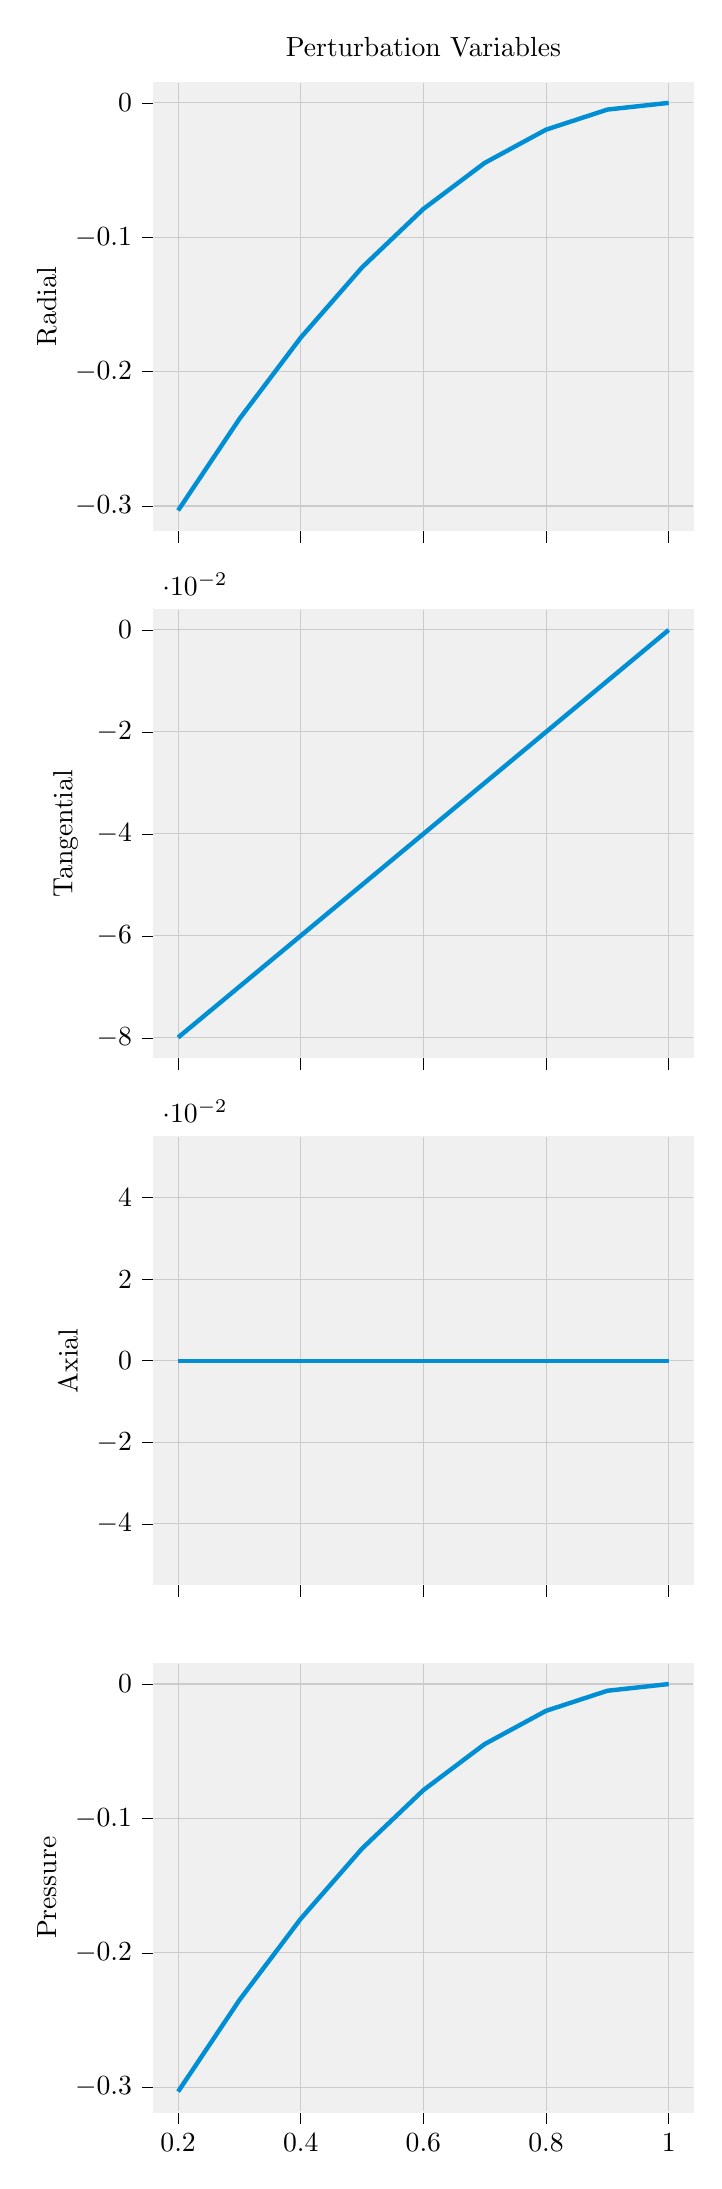
\begin{tikzpicture}

\definecolor{color0}{rgb}{0,0.56078431372549,0.835294117647059}

\begin{groupplot}[group style={group size=1 by 4}]
\nextgroupplot[
axis background/.style={fill=white!94.1176470588235!black},
axis line style={white!94.1176470588235!black},
scaled x ticks=manual:{}{\pgfmathparse{#1}},
tick align=outside,
tick pos=left,
title={Perturbation Variables},
x grid style={white!79.6078431372549!black},
xmajorgrids,
xmin=0.16, xmax=1.04,
xtick style={color=black},
xticklabels={},
y grid style={white!79.6078431372549!black},
ylabel={Radial},
ymajorgrids,
ymin=-0.318457955185476, ymax=0.0151646645326417,
ytick style={color=black}
]
\addplot [ultra thick, color0]
table {%
0.2 -0.303293290652835
0.3 -0.235157812715512
0.4 -0.174664385090322
0.5 -0.122417438109627
0.6 -0.0789390059971149
0.7 -0.044663510874394
0.8 -0.0199334221587584
0.9 -0.00499583472197418
1 0
};

\nextgroupplot[
axis background/.style={fill=white!94.1176470588235!black},
axis line style={white!94.1176470588235!black},
scaled x ticks=manual:{}{\pgfmathparse{#1}},
tick align=outside,
tick pos=left,
x grid style={white!79.6078431372549!black},
xmajorgrids,
xmin=0.16, xmax=1.04,
xtick style={color=black},
xticklabels={},
y grid style={white!79.6078431372549!black},
ylabel={Tangential},
ymajorgrids,
ymin=-0.0839104299153256, ymax=0.00399573475787265,
ytick style={color=black}
]
\addplot [ultra thick, color0]
table {%
0.2 -0.0799146951574529
0.3 -0.0699428483780595
0.4 -0.0599640073719054
0.5 -0.0499791700148053
0.6 -0.0399893347822038
0.7 -0.0299955006493293
0.8 -0.0199986669912967
0.9 -0.00999983348317081
1 0
};

\nextgroupplot[
axis background/.style={fill=white!94.1176470588235!black},
axis line style={white!94.1176470588235!black},
scaled x ticks=manual:{}{\pgfmathparse{#1}},
tick align=outside,
tick pos=left,
x grid style={white!79.6078431372549!black},
xmajorgrids,
xmin=0.16, xmax=1.04,
xtick style={color=black},
xticklabels={},
y grid style={white!79.6078431372549!black},
ylabel={Axial},
ymajorgrids,
ymin=-0.055, ymax=0.055,
ytick style={color=black}
]
\addplot [ultra thick, color0]
table {%
0.2 -0
0.3 -0
0.4 -0
0.5 -0
0.6 -0
0.7 -0
0.8 -0
0.9 -0
1 0
};

\nextgroupplot[
axis background/.style={fill=white!94.1176470588235!black},
axis line style={white!94.1176470588235!black},
tick align=outside,
tick pos=left,
x grid style={white!79.6078431372549!black},
xmajorgrids,
xmin=0.16, xmax=1.04,
xtick style={color=black},
y grid style={white!79.6078431372549!black},
ylabel={Pressure},
ymajorgrids,
ymin=-0.318457955185476, ymax=0.0151646645326417,
ytick style={color=black}
]
\addplot [ultra thick, color0]
table {%
0.2 -0.303293290652835
0.3 -0.235157812715512
0.4 -0.174664385090322
0.5 -0.122417438109627
0.6 -0.0789390059971149
0.7 -0.044663510874394
0.8 -0.0199334221587584
0.9 -0.00499583472197418
1 0
};
\end{groupplot}

\end{tikzpicture}
}
     \end{center}
 \end{figure}

 \begin{figure}
     \begin{center}
         \scalebox{0.75}{% This file was created with tikzplotlib v0.9.12.
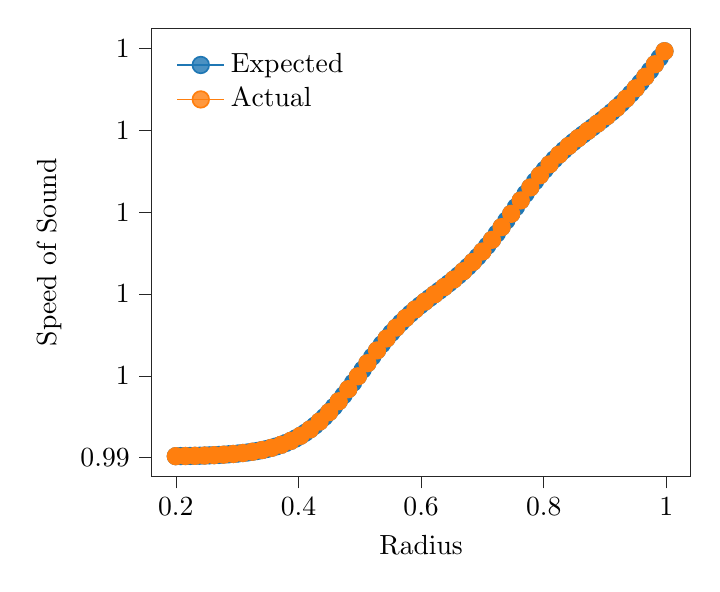
\begin{tikzpicture}

\definecolor{color0}{rgb}{0.12156862745098,0.466666666666667,0.705882352941177}
\definecolor{color1}{rgb}{1,0.498039215686275,0.0549019607843137}

\begin{axis}[
axis line style={white!15!black},
legend cell align={left},
legend style={
  fill opacity=0.8,
  draw opacity=1,
  text opacity=1,
  at={(0.03,0.97)},
  anchor=north west,
  draw=none
},
tick align=outside,
tick pos=left,
x grid style={white!80!black},
xlabel={Radius},
xmin=0.16, xmax=1.04,
xtick style={color=white!15!black},
y grid style={white!80!black},
ylabel={Speed of Sound},
ymin=0.994769378140404, ymax=1.00024907723141,
ytick style={color=white!15!black}
]
\addplot [semithick, color0, mark=*, mark size=3, mark repeat=5, mark options={solid}]
table {%
0.2 0.995018455371813
0.2015625 0.995018613017789
0.203125 0.995018775642226
0.2046875 0.995018943401502
0.20625 0.995019116456855
0.2078125 0.995019294974526
0.209375 0.995019479125914
0.2109375 0.995019669087732
0.2125 0.995019865042164
0.2140625 0.995020067177035
0.215625 0.995020275685978
0.2171875 0.995020490768609
0.21875 0.995020712630706
0.2203125 0.995020941484393
0.221875 0.995021177548333
0.2234375 0.99502142104792
0.225 0.995021672215478
0.2265625 0.995021931290472
0.228125 0.995022198519715
0.2296875 0.995022474157586
0.23125 0.995022758466254
0.2328125 0.995023051715909
0.234375 0.995023354184993
0.2359375 0.995023666160445
0.2375 0.995023987937948
0.2390625 0.995024319822184
0.240625 0.995024662127092
0.2421875 0.99502501517614
0.24375 0.995025379302598
0.2453125 0.995025754849821
0.246875 0.995026142171533
0.2484375 0.99502654163213
0.25 0.995026953606976
0.2515625 0.995027378482722
0.253125 0.995027816657616
0.2546875 0.995028268541835
0.25625 0.995028734557814
0.2578125 0.995029215140593
0.259375 0.995029710738159
0.2609375 0.99503022181181
0.2625 0.995030748836517
0.2640625 0.995031292301296
0.265625 0.995031852709594
0.2671875 0.995032430579672
0.26875 0.995033026445009
0.2703125 0.995033640854704
0.271875 0.995034274373891
0.2734375 0.995034927584162
0.275 0.995035601083997
0.2765625 0.9950362954892
0.278125 0.995037011433347
0.2796875 0.995037749568242
0.28125 0.995038510564377
0.2828125 0.995039295111398
0.284375 0.995040103918589
0.2859375 0.99504093771535
0.2875 0.995041797251693
0.2890625 0.995042683298734
0.290625 0.995043596649204
0.2921875 0.995044538117953
0.29375 0.995045508542472
0.2953125 0.99504650878341
0.296875 0.995047539725102
0.2984375 0.995048602276104
0.3 0.995049697369718
0.3015625 0.99505082596454
0.303125 0.995051989044996
0.3046875 0.995053187621882
0.30625 0.995054422732912
0.3078125 0.99505569544326
0.309375 0.995057006846105
0.3109375 0.995058358063166
0.3125 0.99505975024525
0.3140625 0.99506118457278
0.315625 0.99506266225633
0.3171875 0.995064184537142
0.31875 0.995065752687652
0.3203125 0.995067368011985
0.321875 0.995069031846462
0.3234375 0.995070745560074
0.325 0.995072510554959
0.3265625 0.995074328266849
0.328125 0.995076200165508
0.3296875 0.995078127755144
0.33125 0.995080112574803
0.3328125 0.995082156198734
0.334375 0.995084260236728
0.3359375 0.995086426334427
0.3375 0.995088656173599
0.3390625 0.995090951472378
0.340625 0.995093313985466
0.3421875 0.995095745504288
0.34375 0.995098247857104
0.3453125 0.995100822909076
0.346875 0.995103472562276
0.3484375 0.995106198755638
0.35 0.995109003464851
0.3515625 0.995111888702186
0.353125 0.995114856516256
0.3546875 0.995117908991698
0.35625 0.99512104824878
0.3578125 0.995124276442923
0.359375 0.995127595764138
0.3609375 0.995131008436366
0.3625 0.995134516716721
0.3640625 0.995138122894633
0.365625 0.99514182929088
0.3671875 0.995145638256504
0.36875 0.995149552171609
0.3703125 0.995153573444038
0.371875 0.995157704507913
0.3734375 0.995161947822041
0.375 0.995166305868181
0.3765625 0.99517078114916
0.378125 0.995175376186839
0.3796875 0.995180093519919
0.38125 0.995184935701583
0.3828125 0.995189905296973
0.384375 0.995195004880492
0.3859375 0.995200237032921
0.3875 0.995205604338371
0.3890625 0.995211109381028
0.390625 0.995216754741722
0.3921875 0.995222542994296
0.39375 0.995228476701786
0.3953125 0.995234558412394
0.396875 0.995240790655265
0.3984375 0.995247175936068
0.4 0.995253716732368
0.4015625 0.995260415488804
0.403125 0.995267274612066
0.4046875 0.995274296465674
0.40625 0.995281483364568
0.4078125 0.995288837569503
0.409375 0.995296361281272
0.4109375 0.995304056634736
0.4125 0.995311925692705
0.4140625 0.99531997043964
0.415625 0.995328192775225
0.4171875 0.995336594507788
0.41875 0.995345177347606
0.4203125 0.995353942900101
0.421875 0.995362892658941
0.4234375 0.995372027999073
0.425 0.995381350169694
0.4265625 0.995390860287195
0.428125 0.995400559328093
0.4296875 0.995410448121971
0.43125 0.995420527344466
0.4328125 0.995430797510316
0.434375 0.995441258966504
0.4359375 0.995451911885528
0.4375 0.99546275625882
0.4390625 0.99547379189036
0.440625 0.995485018390503
0.4421875 0.995496435170068
0.44375 0.995508041434705
0.4453125 0.995519836179596
0.446875 0.995531818184506
0.4484375 0.995543986009232
0.45 0.995556337989483
0.4515625 0.99556887223322
0.453125 0.995581586617498
0.4546875 0.995594478785833
0.45625 0.995607546146143
0.4578125 0.995620785869274
0.459375 0.995634194888158
0.4609375 0.995647769897611
0.4625 0.995661507354817
0.4640625 0.995675403480507
0.465625 0.99568945426085
0.4671875 0.995703655450086
0.46875 0.995718002573898
0.4703125 0.99573249093355
0.471875 0.995747115610777
0.4734375 0.99576187147345
0.475 0.995776753181996
0.4765625 0.995791755196583
0.478125 0.995806871785038
0.4796875 0.995822097031516
0.48125 0.995837424845859
0.4828125 0.995852848973668
0.484375 0.995868363007016
0.4859375 0.995883960395803
0.4875 0.995899634459703
0.4890625 0.995915378400664
0.490625 0.995931185315918
0.4921875 0.99594704821146
0.49375 0.995962960015935
0.4953125 0.995978913594894
0.496875 0.99599490176535
0.4984375 0.99601091731059
0.5 0.996026952995172
0.5015625 0.996043001580055
0.503125 0.9960590558378
0.5046875 0.996075108567772
0.50625 0.996091152611297
0.5078125 0.996107180866696
0.509375 0.996123186304151
0.5109375 0.996139161980328
0.5125 0.996155101052716
0.5140625 0.996170996793616
0.515625 0.996186842603728
0.5171875 0.996202632025296
0.51875 0.996218358754747
0.5203125 0.996234016654797
0.521875 0.996249599765976
0.5234375 0.996265102317534
0.525 0.996280518737706
0.5265625 0.996295843663294
0.528125 0.996311071948558
0.5296875 0.996326198673381
0.53125 0.996341219150708
0.5328125 0.996356128933238
0.534375 0.996370923819364
0.5359375 0.996385599858368
0.5375 0.996400153354854
0.5390625 0.996414580872448
0.540625 0.996428879236751
0.5421875 0.996443045537583
0.54375 0.996457077130504
0.5453125 0.996470971637658
0.546875 0.996484726947948
0.5484375 0.996498341216568
0.55 0.996511812863922
0.5515625 0.996525140573951
0.553125 0.996538323291907
0.5546875 0.996551360221601
0.55625 0.996564250822158
0.5578125 0.996576994804306
0.559375 0.996589592126248
0.5609375 0.996602042989138
0.5625 0.996614347832194
0.5640625 0.996626507327495
0.565625 0.996638522374488
0.5671875 0.996650394094226
0.56875 0.996662123823399
0.5703125 0.996673713108157
0.571875 0.996685163697777
0.5734375 0.996696477538195
0.575 0.996707656765432
0.5765625 0.996718703698941
0.578125 0.996729620834897
0.5796875 0.996740410839457
0.58125 0.996751076542014
0.5828125 0.996761620928456
0.584375 0.996772047134458
0.5859375 0.996782358438816
0.5875 0.996792558256849
0.5890625 0.996802650133868
0.590625 0.996812637738736
0.5921875 0.996822524857518
0.59375 0.996832315387248
0.5953125 0.996842013329795
0.596875 0.996851622785849
0.5984375 0.996861147949038
0.6 0.996870593100158
0.6015625 0.996879962601529
0.603125 0.996889260891485
0.6046875 0.996898492478982
0.60625 0.996907661938324
0.6078125 0.996916773904018
0.609375 0.996925833065737
0.6109375 0.99693484416339
0.6125 0.996943811982298
0.6140625 0.996952741348472
0.615625 0.996961637123967
0.6171875 0.996970504202327
0.61875 0.996979347504097
0.6203125 0.996988171972398
0.621875 0.99699698256856
0.6234375 0.997005784267785
0.625 0.99701458205486
0.6265625 0.997023380919878
0.628125 0.997032185853978
0.6296875 0.997041001845085
0.63125 0.997049833873637
0.6328125 0.997058686908295
0.634375 0.997067565901624
0.6359375 0.997076475785728
0.6375 0.997085421467834
0.6390625 0.997094407825827
0.640625 0.997103439703696
0.6421875 0.997112521906918
0.64375 0.997121659197749
0.6453125 0.997130856290419
0.646875 0.99714011784623
0.6484375 0.997149448468545
0.65 0.997158852697664
0.6515625 0.997168335005585
0.653125 0.997177899790646
0.6546875 0.997187551372043
0.65625 0.997197293984224
0.6578125 0.997207131771163
0.659375 0.99721706878051
0.6609375 0.997227108957625
0.6625 0.997237256139491
0.6640625 0.997247514048525
0.665625 0.99725788628628
0.6671875 0.997268376327057
0.66875 0.997278987511436
0.6703125 0.997289723039727
0.671875 0.997300585965368
0.6734375 0.997311579188284
0.675 0.997322705448209
0.6765625 0.99733396731801
0.678125 0.997345367197015
0.6796875 0.997356907304385
0.68125 0.997368589672534
0.6828125 0.997380416140637
0.684375 0.997392388348244
0.6859375 0.997404507729037
0.6875 0.997416775504743
0.6890625 0.997429192679254
0.690625 0.997441760032968
0.6921875 0.997454478117396
0.69375 0.997467347250056
0.6953125 0.997480367509701
0.696875 0.997493538731904
0.6984375 0.997506860505045
0.7 0.997520332166715
0.7015625 0.997533952800602
0.703125 0.997547721233861
0.7046875 0.997561636035014
0.70625 0.997575695512422
0.7078125 0.99758989771334
0.709375 0.99760424042359
0.7109375 0.997618721167887
0.7125 0.997633337210834
0.7140625 0.997648085558606
0.715625 0.997662962961351
0.7171875 0.997677965916316
0.71875 0.99769309067171
0.7203125 0.99770833323133
0.721875 0.997723689359923
0.7234375 0.997739154589328
0.725 0.997754724225353
0.7265625 0.997770393355417
0.728125 0.997786156856923
0.7296875 0.997802009406352
0.73125 0.997817945489074
0.7328125 0.997833959409824
0.734375 0.997850045303847
0.7359375 0.997866197148656
0.7375 0.997882408776374
0.7390625 0.997898673886634
0.740625 0.997914986059968
0.7421875 0.997931338771662
0.74375 0.997947725406015
0.7453125 0.99796413927095
0.746875 0.997980573612922
0.7484375 0.997997021632078
0.75 0.998013476497586
0.7515625 0.998029931363093
0.753125 0.99804637938225
0.7546875 0.998062813724222
0.75625 0.998079227589157
0.7578125 0.99809561422351
0.759375 0.998111966935204
0.7609375 0.998128279108538
0.7625 0.998144544218798
0.7640625 0.998160755846516
0.765625 0.998176907691324
0.7671875 0.998192993585348
0.76875 0.998209007506098
0.7703125 0.99822494358882
0.771875 0.998240796138249
0.7734375 0.998256559639754
0.775 0.998272228769819
0.7765625 0.998287798405844
0.778125 0.998303263635249
0.7796875 0.998318619763842
0.78125 0.998333862323462
0.7828125 0.998348987078856
0.784375 0.998363990033821
0.7859375 0.998378867436566
0.7875 0.998393615784338
0.7890625 0.998408231827285
0.790625 0.998422712571582
0.7921875 0.998437055281832
0.79375 0.998451257482749
0.7953125 0.998465316960158
0.796875 0.998479231761311
0.7984375 0.998493000194569
0.8 0.998506620828457
0.8015625 0.998520092490127
0.803125 0.998533414263267
0.8046875 0.998546585485471
0.80625 0.998559605745116
0.8078125 0.998572474877776
0.809375 0.998585192962203
0.8109375 0.998597760315918
0.8125 0.998610177490429
0.8140625 0.998622445266135
0.815625 0.998634564646928
0.8171875 0.998646536854535
0.81875 0.998658363322638
0.8203125 0.998670045690787
0.821875 0.998681585798157
0.8234375 0.998692985677162
0.825 0.998704247546962
0.8265625 0.998715373806888
0.828125 0.998726367029804
0.8296875 0.998737229955445
0.83125 0.998747965483736
0.8328125 0.998758576668115
0.834375 0.998769066708892
0.8359375 0.998779438946647
0.8375 0.998789696855681
0.8390625 0.998799844037547
0.840625 0.998809884214662
0.8421875 0.998819821224009
0.84375 0.998829659010948
0.8453125 0.998839401623129
0.846875 0.998849053204525
0.8484375 0.998858617989587
0.85 0.998868100297508
0.8515625 0.998877504526627
0.853125 0.998886835148942
0.8546875 0.998896096704753
0.85625 0.998905293797423
0.8578125 0.998914431088254
0.859375 0.998923513291476
0.8609375 0.998932545169345
0.8625 0.998941531527338
0.8640625 0.998950477209444
0.865625 0.998959387093547
0.8671875 0.998968266086877
0.86875 0.998977119121535
0.8703125 0.998985951150087
0.871875 0.998994767141194
0.8734375 0.999003572075294
0.875 0.999012370940312
0.8765625 0.999021168727387
0.878125 0.999029970426612
0.8796875 0.999038781022774
0.88125 0.999047605491075
0.8828125 0.999056448792845
0.884375 0.999065315871205
0.8859375 0.9990742116467
0.8875 0.999083141012874
0.8890625 0.999092108831782
0.890625 0.999101119929434
0.8921875 0.999110179091153
0.89375 0.999119291056848
0.8953125 0.99912846051619
0.896875 0.999137692103687
0.8984375 0.999146990393643
0.9 0.999156359895014
0.9015625 0.999165805046133
0.903125 0.999175330209323
0.9046875 0.999184939665377
0.90625 0.999194637607923
0.9078125 0.999204428137654
0.909375 0.999214315256436
0.9109375 0.999224302861304
0.9125 0.999234394738323
0.9140625 0.999244594556356
0.915625 0.999254905860714
0.9171875 0.999265332066716
0.91875 0.999275876453158
0.9203125 0.999286542155715
0.921875 0.999297332160275
0.9234375 0.999308249296231
0.925 0.99931929622974
0.9265625 0.999330475456977
0.928125 0.999341789297395
0.9296875 0.999353239887015
0.93125 0.999364829171772
0.9328125 0.999376558900945
0.934375 0.999388430620684
0.9359375 0.999400445667676
0.9375 0.999412605162978
0.9390625 0.999424910006034
0.940625 0.999437360868924
0.9421875 0.999449958190866
0.94375 0.999462702173014
0.9453125 0.99947559277357
0.946875 0.999488629703265
0.9484375 0.999501812421221
0.95 0.99951514013125
0.9515625 0.999528611778604
0.953125 0.999542226047224
0.9546875 0.999555981357514
0.95625 0.999569875864668
0.9578125 0.999583907457589
0.959375 0.999598073758421
0.9609375 0.999612372122724
0.9625 0.999626799640318
0.9640625 0.999641353136804
0.965625 0.999656029175807
0.9671875 0.999670824061934
0.96875 0.999685733844464
0.9703125 0.999700754321791
0.971875 0.999715881046614
0.9734375 0.999731109331878
0.975 0.999746434257466
0.9765625 0.999761850677638
0.978125 0.999777353229196
0.9796875 0.999792936340375
0.98125 0.999808594240425
0.9828125 0.999824320969876
0.984375 0.999840110391444
0.9859375 0.999855956201556
0.9875 0.999871851942456
0.9890625 0.999887791014844
0.990625 0.999903766691021
0.9921875 0.999919772128476
0.99375 0.999935800383875
0.9953125 0.9999518444274
0.996875 0.999967897157372
0.9984375 0.999983951415117
1 1
};
\addlegendentry{Expected}
\addplot [semithick, color1, mark=*, mark size=3, mark repeat=10, mark options={solid}]
table {%
0.2 0.995018456864923
0.2015625 0.995018614523536
0.203125 0.995018777161003
0.2046875 0.995018944933715
0.20625 0.99501911800292
0.2078125 0.995019296534873
0.209375 0.995019480700986
0.2109375 0.995019670677984
0.2125 0.995019866648067
0.2140625 0.995020068799073
0.215625 0.995020277324649
0.2171875 0.995020492424426
0.21875 0.995020714304198
0.2203125 0.995020943176106
0.221875 0.995021179258827
0.2234375 0.995021422777772
0.225 0.995021673965284
0.2265625 0.995021933060844
0.228125 0.995022200311284
0.2296875 0.995022475971
0.23125 0.995022760302182
0.2328125 0.995023053575038
0.234375 0.995023356068032
0.2359375 0.995023668068122
0.2375 0.995023989871012
0.2390625 0.995024321781407
0.240625 0.995024664113268
0.2421875 0.995025017190086
0.24375 0.995025381345155
0.2453125 0.995025756921852
0.246875 0.995026144273928
0.2484375 0.995026543765801
0.25 0.995026955772866
0.2515625 0.995027380681796
0.253125 0.995027818890868
0.2546875 0.995028270810286
0.25625 0.995028736862515
0.2578125 0.995029217482623
0.259375 0.995029713118627
0.2609375 0.995030224231855
0.2625 0.995030751297309
0.2640625 0.995031294804038
0.265625 0.99503185525552
0.2671875 0.99503243317005
0.26875 0.99503302908114
0.2703125 0.995033643537925
0.271875 0.995034277105573
0.2734375 0.995034930365713
0.275 0.995035603916859
0.2765625 0.995036298374854
0.278125 0.995037014373313
0.2796875 0.995037752564077
0.28125 0.995038513617676
0.2828125 0.995039298223797
0.284375 0.995040107091765
0.2859375 0.995040940951021
0.2875 0.995041800551616
0.2890625 0.995042686664711
0.290625 0.995043600083077
0.2921875 0.995044541621609
0.29375 0.995045512117841
0.2953125 0.995046512432465
0.296875 0.995047543449862
0.2984375 0.99504860607863
0.3 0.995049701252118
0.3015625 0.995050829928966
0.303125 0.995051993093644
0.3046875 0.995053191756995
0.30625 0.995054426956779
0.3078125 0.995055699758215
0.309375 0.995057011254524
0.3109375 0.995058362567474
0.3125 0.995059754847914
0.3140625 0.995061189276312
0.315625 0.995062667063285
0.3171875 0.99506418945012
0.31875 0.995065757709292
0.3203125 0.99506737314497
0.321875 0.995069037093513
0.3234375 0.995070750923954
0.325 0.995072516038466
0.3265625 0.995074333872819
0.328125 0.99507620589681
0.3296875 0.995078133614681
0.33125 0.995080118565507
0.3328125 0.995082162323567
0.334375 0.995084266498676
0.3359375 0.9950864327365
0.3375 0.995088662718826
0.3390625 0.995090958163807
0.340625 0.995093320826155
0.3421875 0.995095752497305
0.34375 0.995098255005524
0.3453125 0.995100830215974
0.346875 0.995103480030722
0.3484375 0.995106206388693
0.35 0.995109011265563
0.3515625 0.995111896673582
0.353125 0.995114864661337
0.3546875 0.995117917313431
0.35625 0.995121056750094
0.3578125 0.995124285126698
0.359375 0.9951276046332
0.3609375 0.995131017493478
0.3625 0.995134525964574
0.3640625 0.995138132335837
0.365625 0.995141838927955
0.3671875 0.99514564809187
0.36875 0.995149562207576
0.3703125 0.995153583682793
0.371875 0.995157714951511
0.3734375 0.995161958472392
0.375 0.995166316727038
0.3765625 0.995170792218106
0.378125 0.995175387467276
0.3796875 0.995180105013049
0.38125 0.9951849474084
0.3828125 0.995189917218247
0.384375 0.995195017016749
0.3859375 0.995200249384437
0.3875 0.995205616905148
0.3890625 0.995211122162782
0.390625 0.995216767737866
0.3921875 0.995222556203927
0.39375 0.995228490123664
0.3953125 0.995234572044925
0.396875 0.995240804496489
0.3984375 0.995247189983638
0.4 0.995253730983535
0.4015625 0.995260429940401
0.403125 0.99526728926049
0.4046875 0.995274311306871
0.40625 0.995281498394017
0.4078125 0.995288852782202
0.409375 0.99529637667172
0.4109375 0.995304072196924
0.4125 0.995311941420096
0.4140625 0.995319986325164
0.415625 0.995328208811263
0.4171875 0.995336610686161
0.41875 0.99534519365957
0.4203125 0.995353959336335
0.421875 0.995362909209546
0.4234375 0.995372044653562
0.425 0.995381366916992
0.4265625 0.995390877115639
0.428125 0.99540057622543
0.4296875 0.995410465075365
0.43125 0.995420544340501
0.4328125 0.995430814535005
0.434375 0.9954412760053
0.4359375 0.995451928923333
0.4375 0.995462773280006
0.4390625 0.995473808878784
0.440625 0.99548503532953
0.4421875 0.995496452042593
0.44375 0.995508058223182
0.4453125 0.995519852866066
0.446875 0.995531834750632
0.4484375 0.995544002436335
0.45 0.995556354258577
0.4515625 0.995568888325058
0.453125 0.995581602512612
0.4546875 0.995594494464586
0.45625 0.995607561588774
0.4578125 0.995620801055954
0.459375 0.995634209799041
0.4609375 0.995647784512891
0.4625 0.995661521654788
0.4640625 0.995675417445621
0.465625 0.99568946787178
0.4671875 0.995703668687785
0.46875 0.995718015419666
0.4703125 0.995732503369094
0.471875 0.995747127618279
0.4734375 0.995761883035627
0.475 0.995776764282165
0.4765625 0.99579176581872
0.478125 0.995806881913844
0.4796875 0.995822106652473
0.48125 0.995837433945289
0.4828125 0.995852857538786
0.484375 0.995868371025984
0.4859375 0.995883967857782
0.4875 0.995899641354895
0.4890625 0.995915384720355
0.490625 0.99593119105252
0.4921875 0.995947053358542
0.49375 0.995962964568255
0.4953125 0.995978917548424
0.496875 0.995994905117297
0.4984375 0.996010920059412
0.5 0.996026955140587
0.5015625 0.99604300312305
0.503125 0.996059056780628
0.5046875 0.99607510891395
0.50625 0.996091152365595
0.5078125 0.996107180035124
0.509375 0.996123184893937
0.5109375 0.996139159999895
0.5125 0.996155098511652
0.5140625 0.996170993702643
0.515625 0.996186838974662
0.5171875 0.996202627871006
0.51875 0.996218354089111
0.5203125 0.996234011492654
0.521875 0.996249594123071
0.5234375 0.996265096210469
0.525 0.99628051218388
0.5265625 0.996295836680847
0.528125 0.996311064556308
0.5296875 0.996326190890768
0.53125 0.996341210997726
0.5328125 0.996356120430377
0.534375 0.996370914987546
0.5359375 0.996385590718882
0.5375 0.996400143929298
0.5390625 0.996414571182664
0.540625 0.996428869304768
0.5421875 0.996443035385555
0.54375 0.996457066780654
0.5453125 0.996470961112224
0.546875 0.996484716269127
0.5484375 0.996498330406466
0.55 0.996511801944505
0.5515625 0.996525129566998
0.553125 0.996538312218968
0.5546875 0.996551349103953
0.55625 0.996564239680768
0.5578125 0.996576983659798
0.559375 0.996589580998866
0.5609375 0.99660203189872
0.5625 0.996614336798141
0.5640625 0.996626496368753
0.565625 0.996638511509519
0.5671875 0.996650383340996
0.56875 0.996662113199358
0.5703125 0.996673702630226
0.571875 0.996685153382338
0.5734375 0.996696467401083
0.575 0.996707646821926
0.5765625 0.99671869396376
0.578125 0.996729611322198
0.5796875 0.996740401562836
0.58125 0.996751067514504
0.5828125 0.996761612162531
0.584375 0.996772038642035
0.5859375 0.996782350231264
0.5875 0.996792550344992
0.5890625 0.996802642527993
0.590625 0.9968126304486
0.5921875 0.99682251789236
0.59375 0.996832308755795
0.5953125 0.996842007040272
0.596875 0.996851616845993
0.5984375 0.996861142366104
0.6 0.996870587880929
0.6015625 0.996879957752332
0.603125 0.996889256418196
0.6046875 0.996898488387037
0.60625 0.996907658232732
0.6078125 0.996916770589368
0.609375 0.996925830146206
0.6109375 0.996934841642753
0.6125 0.996943809863939
0.6140625 0.996952739635386
0.615625 0.99696163581877
0.6171875 0.99697050330726
0.61875 0.996979347021034
0.6203125 0.99698817190285
0.621875 0.996996982913674
0.6234375 0.997005785028353
0.625 0.997014583231316
0.6265625 0.997023382512302
0.628125 0.997032187862096
0.6296875 0.997041004268265
0.63125 0.99704983671089
0.6328125 0.997058690158273
0.634375 0.997067569562615
0.6359375 0.997076479855652
0.6375 0.997085425944239
0.6390625 0.997094412705881
0.640625 0.997103444984183
0.6421875 0.99711252758423
0.64375 0.997121665267877
0.6453125 0.997130862748945
0.646875 0.99714012468832
0.6484375 0.997149455688936
0.65 0.997158860290657
0.6515625 0.997168342965035
0.653125 0.997177908109951
0.6546875 0.997187560044134
0.65625 0.997197303001553
0.6578125 0.997207141125697
0.659375 0.997217078463718
0.6609375 0.997227118960468
0.6625 0.997237266452414
0.6640625 0.997247524661449
0.665625 0.997257897188593
0.6671875 0.997268387507609
0.66875 0.99727899895853
0.6703125 0.997289734741115
0.671875 0.99730059790825
0.6734375 0.997311591359303
0.675 0.997322717833452
0.6765625 0.997333979903007
0.678125 0.997345379966744
0.6796875 0.997356920243277
0.68125 0.997368602764477
0.6828125 0.997380429368988
0.684375 0.99739240169584
0.6859375 0.997404521178206
0.6875 0.997416789037325
0.6890625 0.997429206276617
0.690625 0.997441773676031
0.6921875 0.997454491786652
0.69375 0.997467360925601
0.6953125 0.997480381171263
0.696875 0.997493552358877
0.6984375 0.997506874076523
0.7 0.997520345661534
0.7015625 0.99753396619738
0.703125 0.997547734511038
0.7046875 0.997561649170906
0.70625 0.997575708485266
0.7078125 0.997589910501347
0.709375 0.997604253004996
0.7109375 0.997618733521015
0.7125 0.997633349314146
0.7140625 0.997648097390765
0.715625 0.997662974501282
0.7171875 0.997677977143266
0.71875 0.997693101565312
0.7203125 0.997708343771666
0.721875 0.997723699527586
0.7234375 0.997739164365486
0.725 0.997754733591812
0.7265625 0.997770402294681
0.728125 0.997786165352254
0.7296875 0.997802017441832
0.73125 0.997817953049659
0.7328125 0.997833966481399
0.734375 0.997850051873278
0.7359375 0.997866203203838
0.7375 0.997882414306278
0.7390625 0.997898678881348
0.740625 0.997914990510736
0.7421875 0.997931342670917
0.74375 0.997947728747407
0.7453125 0.997964142049373
0.746875 0.997980575824534
0.7484375 0.997997023274316
0.75 0.998013477569174
0.7515625 0.998029931864051
0.753125 0.998046379313888
0.7546875 0.998062813089144
0.75625 0.99807922639124
0.7578125 0.998095612467898
0.759375 0.998111964628282
0.7609375 0.998128276257909
0.7625 0.998144540833252
0.7640625 0.998160751936
0.765625 0.998176903266899
0.7671875 0.998192988659148
0.76875 0.998209002091289
0.7703125 0.998224937699545
0.771875 0.998240789789581
0.7734375 0.998256552847637
0.775 0.998272221551014
0.7765625 0.99828779077787
0.778125 0.998303255616321
0.7796875 0.998318611372813
0.78125 0.998333853579755
0.7828125 0.998348978002408
0.784375 0.998363980645011
0.7859375 0.998378857756161
0.7875 0.998393605833424
0.7890625 0.998408221627209
0.790625 0.998422702143889
0.7921875 0.998437044648206
0.79375 0.998451246664958
0.7953125 0.998465305979993
0.796875 0.998479220640538
0.7984375 0.998492988954873
0.8 0.998506609491393
0.8015625 0.998520081077077
0.803125 0.998533402795392
0.8046875 0.99854657398367
0.80625 0.998559594229989
0.8078125 0.998572463369587
0.809375 0.998585181480849
0.8109375 0.998597748880895
0.8125 0.998610166120808
0.8140625 0.998622433980538
0.815625 0.998634553463502
0.8171875 0.99864652579094
0.81875 0.998658352396024
0.8203125 0.998670034917782
0.821875 0.998681575194859
0.8234375 0.998692975259127
0.825 0.998704237329196
0.8265625 0.998715363803844
0.828125 0.998726357255381
0.8296875 0.998737220422984
0.83125 0.998747956206021
0.8328125 0.998758567657376
0.834375 0.998769057976811
0.8359375 0.998779430504357
0.8375 0.998789688713777
0.8390625 0.998799836206093
0.840625 0.998809876703195
0.8421875 0.998819814041552
0.84375 0.998829652166015
0.8453125 0.998839395123738
0.846875 0.998849047058207
0.8484375 0.998858612203394
0.85 0.998868094878026
0.8515625 0.998877499479986
0.853125 0.998886830480824
0.8546875 0.998896092420405
0.85625 0.998905289901664
0.8578125 0.998914427585486
0.859375 0.998923510185693
0.8609375 0.99893254246414
0.8625 0.998941529225911
0.8640625 0.998950475314613
0.865625 0.998959385607748
0.8671875 0.998968265012175
0.86875 0.998977118459628
0.8703125 0.998985950902307
0.871875 0.998994767308516
0.8734375 0.999003572658335
0.875 0.999012371939332
0.8765625 0.999021170142291
0.878125 0.999029972256951
0.8796875 0.999038783267741
0.88125 0.999047608149509
0.8828125 0.99905645186322
0.884375 0.999065319351633
0.8859375 0.999074215534924
0.8875 0.999083145306264
0.8890625 0.999092113527327
0.890625 0.999101125023737
0.8921875 0.999110184580422
0.89375 0.99911929693689
0.8953125 0.999128466782402
0.896875 0.999137698751044
0.8984375 0.999146997416694
0.9 0.999156367287867
0.9015625 0.999165812802446
0.903125 0.999175338322296
0.9046875 0.999184948127739
0.90625 0.999194646411923
0.9078125 0.999204437275049
0.909375 0.999214324718484
0.9109375 0.999224312638749
0.9125 0.999234404821392
0.9140625 0.999244604934746
0.915625 0.999254916523585
0.9171875 0.999265343002684
0.91875 0.999275887650288
0.9203125 0.999286553601519
0.921875 0.999297343841704
0.9234375 0.999308261199674
0.925 0.999319308341024
0.9265625 0.999330487761368
0.928125 0.9993418017796
0.9296875 0.999353252531186
0.93125 0.999364841961513
0.9328125 0.999376571819322
0.934375 0.999388443650233
0.9359375 0.999400458790422
0.9375 0.999412618360445
0.9390625 0.999424923259268
0.940625 0.999437374158512
0.9421875 0.999449971496964
0.94375 0.999462715475369
0.9453125 0.999475606051554
0.946875 0.999488642935903
0.9484375 0.999501825587232
0.95 0.999515153209081
0.9515625 0.999528624746476
0.953125 0.99954223888317
0.9546875 0.999555994039429
0.95625 0.999569888370357
0.9578125 0.99958391976482
0.959375 0.999598085844975
0.9609375 0.999612383966455
0.9625 0.999626811219206
0.9640625 0.999641364429017
0.965625 0.999656040159762
0.9671875 0.999670834716353
0.96875 0.999685744148442
0.9703125 0.999700764254856
0.971875 0.99971589058879
0.9734375 0.999731118463747
0.975 0.999746442960232
0.9765625 0.999761858933186
0.978125 0.999777361020152
0.9796875 0.999792943650165
0.98125 0.999808601053332
0.9828125 0.999824327271091
0.984375 0.999840116167121
0.9859375 0.999855961438859
0.9875 0.999871856629601
0.9890625 0.999887795141146
0.990625 0.999903770246926
0.9921875 0.999919775105598
0.99375 0.999935802775024
0.9953125 0.999951846226604
0.996875 0.999967898359898
0.9984375 0.999983952017487
1 1
};
\addlegendentry{Actual}
\end{axis}

\end{tikzpicture}
}
     \end{center}
     \caption{Speed of Sound from Integrating the Tangential Mach Number}
 \end{figure}

% \begin{figure}
%     \begin{center}
%         \scalebox{0.75}{\begin{tikzpicture}[gnuplot]
%% generated with GNUPLOT 5.2p8 (Lua 5.3; terminal rev. Nov 2018, script rev. 108)
%% Tue 21 Sep 2021 03:58:20 PM EDT
\path (0.000,0.000) rectangle (12.500,8.750);
\gpcolor{color=gp lt color axes}
\gpsetlinetype{gp lt axes}
\gpsetdashtype{gp dt axes}
\gpsetlinewidth{0.50}
\draw[gp path] (2.240,0.985)--(11.947,0.985);
\gpcolor{color=gp lt color border}
\gpsetlinetype{gp lt border}
\gpsetdashtype{gp dt solid}
\gpsetlinewidth{1.00}
\draw[gp path] (2.240,0.985)--(2.420,0.985);
\draw[gp path] (11.947,0.985)--(11.767,0.985);
\node[gp node right] at (2.056,0.985) {$0$};
\gpcolor{color=gp lt color axes}
\gpsetlinetype{gp lt axes}
\gpsetdashtype{gp dt axes}
\gpsetlinewidth{0.50}
\draw[gp path] (2.240,1.917)--(11.947,1.917);
\gpcolor{color=gp lt color border}
\gpsetlinetype{gp lt border}
\gpsetdashtype{gp dt solid}
\gpsetlinewidth{1.00}
\draw[gp path] (2.240,1.917)--(2.420,1.917);
\draw[gp path] (11.947,1.917)--(11.767,1.917);
\node[gp node right] at (2.056,1.917) {$2\times10^{-9}$};
\gpcolor{color=gp lt color axes}
\gpsetlinetype{gp lt axes}
\gpsetdashtype{gp dt axes}
\gpsetlinewidth{0.50}
\draw[gp path] (2.240,2.849)--(11.947,2.849);
\gpcolor{color=gp lt color border}
\gpsetlinetype{gp lt border}
\gpsetdashtype{gp dt solid}
\gpsetlinewidth{1.00}
\draw[gp path] (2.240,2.849)--(2.420,2.849);
\draw[gp path] (11.947,2.849)--(11.767,2.849);
\node[gp node right] at (2.056,2.849) {$4\times10^{-9}$};
\gpcolor{color=gp lt color axes}
\gpsetlinetype{gp lt axes}
\gpsetdashtype{gp dt axes}
\gpsetlinewidth{0.50}
\draw[gp path] (2.240,3.781)--(11.947,3.781);
\gpcolor{color=gp lt color border}
\gpsetlinetype{gp lt border}
\gpsetdashtype{gp dt solid}
\gpsetlinewidth{1.00}
\draw[gp path] (2.240,3.781)--(2.420,3.781);
\draw[gp path] (11.947,3.781)--(11.767,3.781);
\node[gp node right] at (2.056,3.781) {$6\times10^{-9}$};
\gpcolor{color=gp lt color axes}
\gpsetlinetype{gp lt axes}
\gpsetdashtype{gp dt axes}
\gpsetlinewidth{0.50}
\draw[gp path] (2.240,4.713)--(11.947,4.713);
\gpcolor{color=gp lt color border}
\gpsetlinetype{gp lt border}
\gpsetdashtype{gp dt solid}
\gpsetlinewidth{1.00}
\draw[gp path] (2.240,4.713)--(2.420,4.713);
\draw[gp path] (11.947,4.713)--(11.767,4.713);
\node[gp node right] at (2.056,4.713) {$8\times10^{-9}$};
\gpcolor{color=gp lt color axes}
\gpsetlinetype{gp lt axes}
\gpsetdashtype{gp dt axes}
\gpsetlinewidth{0.50}
\draw[gp path] (2.240,5.645)--(11.947,5.645);
\gpcolor{color=gp lt color border}
\gpsetlinetype{gp lt border}
\gpsetdashtype{gp dt solid}
\gpsetlinewidth{1.00}
\draw[gp path] (2.240,5.645)--(2.420,5.645);
\draw[gp path] (11.947,5.645)--(11.767,5.645);
\node[gp node right] at (2.056,5.645) {$1\times10^{-8}$};
\gpcolor{color=gp lt color axes}
\gpsetlinetype{gp lt axes}
\gpsetdashtype{gp dt axes}
\gpsetlinewidth{0.50}
\draw[gp path] (2.240,6.577)--(11.947,6.577);
\gpcolor{color=gp lt color border}
\gpsetlinetype{gp lt border}
\gpsetdashtype{gp dt solid}
\gpsetlinewidth{1.00}
\draw[gp path] (2.240,6.577)--(2.420,6.577);
\draw[gp path] (11.947,6.577)--(11.767,6.577);
\node[gp node right] at (2.056,6.577) {$1.2\times10^{-8}$};
\gpcolor{color=gp lt color axes}
\gpsetlinetype{gp lt axes}
\gpsetdashtype{gp dt axes}
\gpsetlinewidth{0.50}
\draw[gp path] (2.240,7.509)--(11.947,7.509);
\gpcolor{color=gp lt color border}
\gpsetlinetype{gp lt border}
\gpsetdashtype{gp dt solid}
\gpsetlinewidth{1.00}
\draw[gp path] (2.240,7.509)--(2.420,7.509);
\draw[gp path] (11.947,7.509)--(11.767,7.509);
\node[gp node right] at (2.056,7.509) {$1.4\times10^{-8}$};
\gpcolor{color=gp lt color axes}
\gpsetlinetype{gp lt axes}
\gpsetdashtype{gp dt axes}
\gpsetlinewidth{0.50}
\draw[gp path] (2.240,8.441)--(11.947,8.441);
\gpcolor{color=gp lt color border}
\gpsetlinetype{gp lt border}
\gpsetdashtype{gp dt solid}
\gpsetlinewidth{1.00}
\draw[gp path] (2.240,8.441)--(2.420,8.441);
\draw[gp path] (11.947,8.441)--(11.767,8.441);
\node[gp node right] at (2.056,8.441) {$1.6\times10^{-8}$};
\gpcolor{color=gp lt color axes}
\gpsetlinetype{gp lt axes}
\gpsetdashtype{gp dt axes}
\gpsetlinewidth{0.50}
\draw[gp path] (2.240,0.985)--(2.240,8.441);
\gpcolor{color=gp lt color border}
\gpsetlinetype{gp lt border}
\gpsetdashtype{gp dt solid}
\gpsetlinewidth{1.00}
\draw[gp path] (2.240,0.985)--(2.240,1.165);
\draw[gp path] (2.240,8.441)--(2.240,8.261);
\node[gp node center] at (2.240,0.677) {$0.2$};
\gpcolor{color=gp lt color axes}
\gpsetlinetype{gp lt axes}
\gpsetdashtype{gp dt axes}
\gpsetlinewidth{0.50}
\draw[gp path] (3.453,0.985)--(3.453,8.441);
\gpcolor{color=gp lt color border}
\gpsetlinetype{gp lt border}
\gpsetdashtype{gp dt solid}
\gpsetlinewidth{1.00}
\draw[gp path] (3.453,0.985)--(3.453,1.165);
\draw[gp path] (3.453,8.441)--(3.453,8.261);
\node[gp node center] at (3.453,0.677) {$0.3$};
\gpcolor{color=gp lt color axes}
\gpsetlinetype{gp lt axes}
\gpsetdashtype{gp dt axes}
\gpsetlinewidth{0.50}
\draw[gp path] (4.667,0.985)--(4.667,7.953);
\draw[gp path] (4.667,8.261)--(4.667,8.441);
\gpcolor{color=gp lt color border}
\gpsetlinetype{gp lt border}
\gpsetdashtype{gp dt solid}
\gpsetlinewidth{1.00}
\draw[gp path] (4.667,0.985)--(4.667,1.165);
\draw[gp path] (4.667,8.441)--(4.667,8.261);
\node[gp node center] at (4.667,0.677) {$0.4$};
\gpcolor{color=gp lt color axes}
\gpsetlinetype{gp lt axes}
\gpsetdashtype{gp dt axes}
\gpsetlinewidth{0.50}
\draw[gp path] (5.880,0.985)--(5.880,7.953);
\draw[gp path] (5.880,8.261)--(5.880,8.441);
\gpcolor{color=gp lt color border}
\gpsetlinetype{gp lt border}
\gpsetdashtype{gp dt solid}
\gpsetlinewidth{1.00}
\draw[gp path] (5.880,0.985)--(5.880,1.165);
\draw[gp path] (5.880,8.441)--(5.880,8.261);
\node[gp node center] at (5.880,0.677) {$0.5$};
\gpcolor{color=gp lt color axes}
\gpsetlinetype{gp lt axes}
\gpsetdashtype{gp dt axes}
\gpsetlinewidth{0.50}
\draw[gp path] (7.094,0.985)--(7.094,7.953);
\draw[gp path] (7.094,8.261)--(7.094,8.441);
\gpcolor{color=gp lt color border}
\gpsetlinetype{gp lt border}
\gpsetdashtype{gp dt solid}
\gpsetlinewidth{1.00}
\draw[gp path] (7.094,0.985)--(7.094,1.165);
\draw[gp path] (7.094,8.441)--(7.094,8.261);
\node[gp node center] at (7.094,0.677) {$0.6$};
\gpcolor{color=gp lt color axes}
\gpsetlinetype{gp lt axes}
\gpsetdashtype{gp dt axes}
\gpsetlinewidth{0.50}
\draw[gp path] (8.307,0.985)--(8.307,7.953);
\draw[gp path] (8.307,8.261)--(8.307,8.441);
\gpcolor{color=gp lt color border}
\gpsetlinetype{gp lt border}
\gpsetdashtype{gp dt solid}
\gpsetlinewidth{1.00}
\draw[gp path] (8.307,0.985)--(8.307,1.165);
\draw[gp path] (8.307,8.441)--(8.307,8.261);
\node[gp node center] at (8.307,0.677) {$0.7$};
\gpcolor{color=gp lt color axes}
\gpsetlinetype{gp lt axes}
\gpsetdashtype{gp dt axes}
\gpsetlinewidth{0.50}
\draw[gp path] (9.520,0.985)--(9.520,7.953);
\draw[gp path] (9.520,8.261)--(9.520,8.441);
\gpcolor{color=gp lt color border}
\gpsetlinetype{gp lt border}
\gpsetdashtype{gp dt solid}
\gpsetlinewidth{1.00}
\draw[gp path] (9.520,0.985)--(9.520,1.165);
\draw[gp path] (9.520,8.441)--(9.520,8.261);
\node[gp node center] at (9.520,0.677) {$0.8$};
\gpcolor{color=gp lt color axes}
\gpsetlinetype{gp lt axes}
\gpsetdashtype{gp dt axes}
\gpsetlinewidth{0.50}
\draw[gp path] (10.734,0.985)--(10.734,7.953);
\draw[gp path] (10.734,8.261)--(10.734,8.441);
\gpcolor{color=gp lt color border}
\gpsetlinetype{gp lt border}
\gpsetdashtype{gp dt solid}
\gpsetlinewidth{1.00}
\draw[gp path] (10.734,0.985)--(10.734,1.165);
\draw[gp path] (10.734,8.441)--(10.734,8.261);
\node[gp node center] at (10.734,0.677) {$0.9$};
\gpcolor{color=gp lt color axes}
\gpsetlinetype{gp lt axes}
\gpsetdashtype{gp dt axes}
\gpsetlinewidth{0.50}
\draw[gp path] (11.947,0.985)--(11.947,8.441);
\gpcolor{color=gp lt color border}
\gpsetlinetype{gp lt border}
\gpsetdashtype{gp dt solid}
\gpsetlinewidth{1.00}
\draw[gp path] (11.947,0.985)--(11.947,1.165);
\draw[gp path] (11.947,8.441)--(11.947,8.261);
\node[gp node center] at (11.947,0.677) {$1$};
\draw[gp path] (2.240,8.441)--(2.240,0.985)--(11.947,0.985)--(11.947,8.441)--cycle;
\node[gp node center,rotate=-270] at (0.292,4.713) {Sound Speed Error};
\node[gp node center] at (7.093,0.215) {Radius [-]};
\node[gp node right] at (10.479,8.107) {"../SoundSpeedError.dat" using 1:2};
\gpcolor{rgb color={0.165,0.518,0.647}}
\draw[gp path] (10.663,8.107)--(11.579,8.107);
\draw[gp path] (2.240,1.173)--(2.249,1.027)--(2.259,1.088)--(2.268,1.233)--(2.278,1.377)%
  --(2.287,1.522)--(2.297,1.665)--(2.306,1.809)--(2.316,1.952)--(2.325,2.094)--(2.335,2.235)%
  --(2.344,2.376)--(2.354,2.516)--(2.363,2.655)--(2.373,2.793)--(2.382,2.930)--(2.392,3.066)%
  --(2.401,3.200)--(2.411,3.334)--(2.420,3.466)--(2.430,3.597)--(2.439,3.726)--(2.449,3.854)%
  --(2.458,3.980)--(2.468,4.105)--(2.477,4.228)--(2.486,4.350)--(2.496,4.469)--(2.505,4.587)%
  --(2.515,4.703)--(2.524,4.817)--(2.534,4.930)--(2.543,5.040)--(2.553,5.148)--(2.562,5.254)%
  --(2.572,5.359)--(2.581,5.460)--(2.591,5.560)--(2.600,5.658)--(2.610,5.753)--(2.619,5.846)%
  --(2.629,5.937)--(2.638,6.026)--(2.648,6.112)--(2.657,6.196)--(2.667,6.277)--(2.676,6.357)%
  --(2.686,6.433)--(2.695,6.508)--(2.704,6.579)--(2.714,6.649)--(2.723,6.716)--(2.733,6.780)%
  --(2.742,6.842)--(2.752,6.902)--(2.761,6.959)--(2.771,7.014)--(2.780,7.066)--(2.790,7.116)%
  --(2.799,7.163)--(2.809,7.208)--(2.818,7.251)--(2.828,7.291)--(2.837,7.328)--(2.847,7.363)%
  --(2.856,7.396)--(2.866,7.427)--(2.875,7.455)--(2.885,7.480)--(2.894,7.504)--(2.904,7.525)%
  --(2.913,7.543)--(2.923,7.560)--(2.932,7.574)--(2.941,7.586)--(2.951,7.596)--(2.960,7.603)%
  --(2.970,7.609)--(2.979,7.612)--(2.989,7.613)--(2.998,7.612)--(3.008,7.609)--(3.017,7.604)%
  --(3.027,7.597)--(3.036,7.588)--(3.046,7.577)--(3.055,7.565)--(3.065,7.550)--(3.074,7.533)%
  --(3.084,7.515)--(3.093,7.495)--(3.103,7.473)--(3.112,7.450)--(3.122,7.424)--(3.131,7.397)%
  --(3.141,7.369)--(3.150,7.339)--(3.160,7.307)--(3.169,7.274)--(3.178,7.239)--(3.188,7.203)%
  --(3.197,7.166)--(3.207,7.127)--(3.216,7.086)--(3.226,7.045)--(3.235,7.002)--(3.245,6.958)%
  --(3.254,6.912)--(3.264,6.866)--(3.273,6.818)--(3.283,6.769)--(3.292,6.719)--(3.302,6.668)%
  --(3.311,6.616)--(3.321,6.563)--(3.330,6.508)--(3.340,6.453)--(3.349,6.397)--(3.359,6.340)%
  --(3.368,6.283)--(3.378,6.224)--(3.387,6.164)--(3.396,6.104)--(3.406,6.043)--(3.415,5.981)%
  --(3.425,5.919)--(3.434,5.855)--(3.444,5.791)--(3.453,5.727)--(3.463,5.662)--(3.472,5.596)%
  --(3.482,5.529)--(3.491,5.462)--(3.501,5.395)--(3.510,5.327)--(3.520,5.258)--(3.529,5.189)%
  --(3.539,5.120)--(3.548,5.050)--(3.558,4.979)--(3.567,4.909)--(3.577,4.837)--(3.586,4.766)%
  --(3.596,4.694)--(3.605,4.622)--(3.615,4.549)--(3.624,4.476)--(3.633,4.403)--(3.643,4.329)%
  --(3.652,4.256)--(3.662,4.181)--(3.671,4.107)--(3.681,4.033)--(3.690,3.958)--(3.700,3.883)%
  --(3.709,3.808)--(3.719,3.732)--(3.728,3.657)--(3.738,3.581)--(3.747,3.505)--(3.757,3.429)%
  --(3.766,3.353)--(3.776,3.276)--(3.785,3.200)--(3.795,3.123)--(3.804,3.046)--(3.814,2.969)%
  --(3.823,2.893)--(3.833,2.815)--(3.842,2.738)--(3.852,2.661)--(3.861,2.584)--(3.870,2.506)%
  --(3.880,2.429)--(3.889,2.351)--(3.899,2.274)--(3.908,2.196)--(3.918,2.118)--(3.927,2.041)%
  --(3.937,1.963)--(3.946,1.885)--(3.956,1.807)--(3.965,1.729)--(3.975,1.651)--(3.984,1.573)%
  --(3.994,1.495)--(4.003,1.417)--(4.013,1.339)--(4.022,1.261)--(4.032,1.183)--(4.041,1.105)%
  --(4.051,1.027)--(4.060,1.021)--(4.070,1.099)--(4.079,1.177)--(4.089,1.255)--(4.098,1.333)%
  --(4.107,1.411)--(4.117,1.489)--(4.126,1.567)--(4.136,1.645)--(4.145,1.723)--(4.155,1.801)%
  --(4.164,1.879)--(4.174,1.957)--(4.183,2.035)--(4.193,2.112)--(4.202,2.190)--(4.212,2.268)%
  --(4.221,2.345)--(4.231,2.423)--(4.240,2.500)--(4.250,2.578)--(4.259,2.655)--(4.269,2.732)%
  --(4.278,2.809)--(4.288,2.887)--(4.297,2.963)--(4.307,3.040)--(4.316,3.117)--(4.325,3.194)%
  --(4.335,3.270)--(4.344,3.347)--(4.354,3.423)--(4.363,3.499)--(4.373,3.575)--(4.382,3.651)%
  --(4.392,3.726)--(4.401,3.802)--(4.411,3.877)--(4.420,3.952)--(4.430,4.027)--(4.439,4.102)%
  --(4.449,4.176)--(4.458,4.250)--(4.468,4.324)--(4.477,4.398)--(4.487,4.471)--(4.496,4.544)%
  --(4.506,4.617)--(4.515,4.689)--(4.525,4.761)--(4.534,4.833)--(4.544,4.904)--(4.553,4.975)%
  --(4.562,5.046)--(4.572,5.116)--(4.581,5.186)--(4.591,5.255)--(4.600,5.324)--(4.610,5.392)%
  --(4.619,5.460)--(4.629,5.527)--(4.638,5.594)--(4.648,5.660)--(4.657,5.726)--(4.667,5.791)%
  --(4.676,5.855)--(4.686,5.919)--(4.695,5.981)--(4.705,6.044)--(4.714,6.105)--(4.724,6.166)%
  --(4.733,6.226)--(4.743,6.285)--(4.752,6.343)--(4.762,6.401)--(4.771,6.458)--(4.781,6.513)%
  --(4.790,6.568)--(4.799,6.622)--(4.809,6.675)--(4.818,6.726)--(4.828,6.777)--(4.837,6.827)%
  --(4.847,6.875)--(4.856,6.922)--(4.866,6.969)--(4.875,7.014)--(4.885,7.057)--(4.894,7.100)%
  --(4.904,7.141)--(4.913,7.181)--(4.923,7.219)--(4.932,7.256)--(4.942,7.292)--(4.951,7.326)%
  --(4.961,7.359)--(4.970,7.390)--(4.980,7.420)--(4.989,7.448)--(4.999,7.474)--(5.008,7.499)%
  --(5.017,7.522)--(5.027,7.543)--(5.036,7.562)--(5.046,7.580)--(5.055,7.596)--(5.065,7.610)%
  --(5.074,7.623)--(5.084,7.633)--(5.093,7.641)--(5.103,7.648)--(5.112,7.652)--(5.122,7.654)%
  --(5.131,7.655)--(5.141,7.653)--(5.150,7.649)--(5.160,7.643)--(5.169,7.635)--(5.179,7.625)%
  --(5.188,7.612)--(5.198,7.597)--(5.207,7.580)--(5.217,7.561)--(5.226,7.539)--(5.236,7.515)%
  --(5.245,7.489)--(5.254,7.460)--(5.264,7.429)--(5.273,7.396)--(5.283,7.360)--(5.292,7.322)%
  --(5.302,7.281)--(5.311,7.238)--(5.321,7.192)--(5.330,7.144)--(5.340,7.094)--(5.349,7.041)%
  --(5.359,6.986)--(5.368,6.928)--(5.378,6.868)--(5.387,6.805)--(5.397,6.740)--(5.406,6.672)%
  --(5.416,6.602)--(5.425,6.530)--(5.435,6.455)--(5.444,6.378)--(5.454,6.298)--(5.463,6.216)%
  --(5.473,6.131)--(5.482,6.045)--(5.491,5.956)--(5.501,5.864)--(5.510,5.770)--(5.520,5.675)%
  --(5.529,5.576)--(5.539,5.476)--(5.548,5.374)--(5.558,5.269)--(5.567,5.162)--(5.577,5.054)%
  --(5.586,4.943)--(5.596,4.830)--(5.605,4.716)--(5.615,4.599)--(5.624,4.481)--(5.634,4.361)%
  --(5.643,4.239)--(5.653,4.116)--(5.662,3.990)--(5.672,3.864)--(5.681,3.736)--(5.691,3.606)%
  --(5.700,3.475)--(5.709,3.342)--(5.719,3.209)--(5.728,3.074)--(5.738,2.938)--(5.747,2.801)%
  --(5.757,2.662)--(5.766,2.523)--(5.776,2.383)--(5.785,2.242)--(5.795,2.101)--(5.804,1.959)%
  --(5.814,1.816)--(5.823,1.672)--(5.833,1.528)--(5.842,1.384)--(5.852,1.239)--(5.861,1.095)%
  --(5.871,1.020)--(5.880,1.166)--(5.890,1.311)--(5.899,1.456)--(5.909,1.601)--(5.918,1.746)%
  --(5.928,1.891)--(5.937,2.035)--(5.946,2.179)--(5.956,2.322)--(5.965,2.465)--(5.975,2.607)%
  --(5.984,2.749)--(5.994,2.890)--(6.003,3.030)--(6.013,3.169)--(6.022,3.307)--(6.032,3.444)%
  --(6.041,3.580)--(6.051,3.715)--(6.060,3.849)--(6.070,3.981)--(6.079,4.112)--(6.089,4.242)%
  --(6.098,4.370)--(6.108,4.497)--(6.117,4.622)--(6.127,4.746)--(6.136,4.868)--(6.146,4.988)%
  --(6.155,5.107)--(6.165,5.223)--(6.174,5.338)--(6.183,5.451)--(6.193,5.562)--(6.202,5.672)%
  --(6.212,5.779)--(6.221,5.884)--(6.231,5.987)--(6.240,6.088)--(6.250,6.187)--(6.259,6.283)%
  --(6.269,6.378)--(6.278,6.470)--(6.288,6.560)--(6.297,6.648)--(6.307,6.734)--(6.316,6.817)%
  --(6.326,6.898)--(6.335,6.977)--(6.345,7.053)--(6.354,7.127)--(6.364,7.199)--(6.373,7.268)%
  --(6.383,7.335)--(6.392,7.400)--(6.401,7.462)--(6.411,7.522)--(6.420,7.580)--(6.430,7.635)%
  --(6.439,7.688)--(6.449,7.739)--(6.458,7.787)--(6.468,7.833)--(6.477,7.877)--(6.487,7.919)%
  --(6.496,7.958)--(6.506,7.995)--(6.515,8.029)--(6.525,8.062)--(6.534,8.092)--(6.544,8.120)%
  --(6.553,8.146)--(6.563,8.170)--(6.572,8.191)--(6.582,8.211)--(6.591,8.228)--(6.601,8.244)%
  --(6.610,8.257)--(6.620,8.269)--(6.629,8.278)--(6.638,8.286)--(6.648,8.291)--(6.657,8.295)%
  --(6.667,8.297)--(6.676,8.297)--(6.686,8.295)--(6.695,8.292)--(6.705,8.287)--(6.714,8.280)%
  --(6.724,8.272)--(6.733,8.261)--(6.743,8.250)--(6.752,8.237)--(6.762,8.222)--(6.771,8.206)%
  --(6.781,8.188)--(6.790,8.169)--(6.800,8.149)--(6.809,8.127)--(6.819,8.104)--(6.828,8.079)%
  --(6.838,8.054)--(6.847,8.027)--(6.857,7.999)--(6.866,7.970)--(6.875,7.940)--(6.885,7.908)%
  --(6.894,7.876)--(6.904,7.843)--(6.913,7.809)--(6.923,7.773)--(6.932,7.737)--(6.942,7.700)%
  --(6.951,7.663)--(6.961,7.624)--(6.970,7.585)--(6.980,7.544)--(6.989,7.504)--(6.999,7.462)%
  --(7.008,7.420)--(7.018,7.377)--(7.027,7.334)--(7.037,7.290)--(7.046,7.245)--(7.056,7.200)%
  --(7.065,7.155)--(7.075,7.109)--(7.084,7.062)--(7.094,7.015)--(7.103,6.968)--(7.112,6.921)%
  --(7.122,6.873)--(7.131,6.825)--(7.141,6.776)--(7.150,6.728)--(7.160,6.679)--(7.169,6.629)%
  --(7.179,6.580)--(7.188,6.530)--(7.198,6.481)--(7.207,6.431)--(7.217,6.381)--(7.226,6.331)%
  --(7.236,6.281)--(7.245,6.230)--(7.255,6.180)--(7.264,6.130)--(7.274,6.079)--(7.283,6.029)%
  --(7.293,5.979)--(7.302,5.929)--(7.312,5.878)--(7.321,5.828)--(7.330,5.778)--(7.340,5.728)%
  --(7.349,5.678)--(7.359,5.629)--(7.368,5.579)--(7.378,5.529)--(7.387,5.480)--(7.397,5.431)%
  --(7.406,5.382)--(7.416,5.333)--(7.425,5.284)--(7.435,5.236)--(7.444,5.188)--(7.454,5.140)%
  --(7.463,5.092)--(7.473,5.044)--(7.482,4.997)--(7.492,4.950)--(7.501,4.903)--(7.511,4.856)%
  --(7.520,4.810)--(7.530,4.764)--(7.539,4.718)--(7.549,4.673)--(7.558,4.628)--(7.567,4.583)%
  --(7.577,4.538)--(7.586,4.494)--(7.596,4.450)--(7.605,4.406)--(7.615,4.363)--(7.624,4.320)%
  --(7.634,4.277)--(7.643,4.235)--(7.653,4.193)--(7.662,4.151)--(7.672,4.109)--(7.681,4.068)%
  --(7.691,4.027)--(7.700,3.987)--(7.710,3.947)--(7.719,3.907)--(7.729,3.868)--(7.738,3.829)%
  --(7.748,3.790)--(7.757,3.751)--(7.767,3.713)--(7.776,3.675)--(7.786,3.638)--(7.795,3.601)%
  --(7.804,3.564)--(7.814,3.528)--(7.823,3.492)--(7.833,3.456)--(7.842,3.421)--(7.852,3.385)%
  --(7.861,3.351)--(7.871,3.316)--(7.880,3.282)--(7.890,3.248)--(7.899,3.215)--(7.909,3.182)%
  --(7.918,3.149)--(7.928,3.117)--(7.937,3.085)--(7.947,3.053)--(7.956,3.021)--(7.966,2.990)%
  --(7.975,2.959)--(7.985,2.928)--(7.994,2.898)--(8.004,2.868)--(8.013,2.839)--(8.022,2.809)%
  --(8.032,2.780)--(8.041,2.751)--(8.051,2.723)--(8.060,2.695)--(8.070,2.667)--(8.079,2.639)%
  --(8.089,2.612)--(8.098,2.585)--(8.108,2.558)--(8.117,2.531)--(8.127,2.505)--(8.136,2.479)%
  --(8.146,2.453)--(8.155,2.428)--(8.165,2.403)--(8.174,2.378)--(8.184,2.353)--(8.193,2.328)%
  --(8.203,2.304)--(8.212,2.280)--(8.222,2.256)--(8.231,2.233)--(8.241,2.210)--(8.250,2.187)%
  --(8.259,2.164)--(8.269,2.141)--(8.278,2.119)--(8.288,2.097)--(8.297,2.075)--(8.307,2.053)%
  --(8.316,2.031)--(8.326,2.010)--(8.335,1.989)--(8.345,1.968)--(8.354,1.947)--(8.364,1.926)%
  --(8.373,1.906)--(8.383,1.886)--(8.392,1.866)--(8.402,1.846)--(8.411,1.826)--(8.421,1.807)%
  --(8.430,1.787)--(8.440,1.768)--(8.449,1.749)--(8.459,1.730)--(8.468,1.712)--(8.478,1.693)%
  --(8.487,1.675)--(8.496,1.656)--(8.506,1.638)--(8.515,1.620)--(8.525,1.602)--(8.534,1.585)%
  --(8.544,1.567)--(8.553,1.550)--(8.563,1.532)--(8.572,1.515)--(8.582,1.498)--(8.591,1.481)%
  --(8.601,1.464)--(8.610,1.447)--(8.620,1.430)--(8.629,1.414)--(8.639,1.397)--(8.648,1.381)%
  --(8.658,1.365)--(8.667,1.348)--(8.677,1.332)--(8.686,1.316)--(8.696,1.300)--(8.705,1.284)%
  --(8.714,1.268)--(8.724,1.252)--(8.733,1.237)--(8.743,1.221)--(8.752,1.205)--(8.762,1.190)%
  --(8.771,1.174)--(8.781,1.159)--(8.790,1.143)--(8.800,1.128)--(8.809,1.112)--(8.819,1.097)%
  --(8.828,1.082)--(8.838,1.067)--(8.847,1.051)--(8.857,1.036)--(8.866,1.021)--(8.876,1.006)%
  --(8.885,0.991)--(8.895,0.995)--(8.904,1.010)--(8.914,1.025)--(8.923,1.040)--(8.933,1.055)%
  --(8.942,1.070)--(8.951,1.085)--(8.961,1.101)--(8.970,1.116)--(8.980,1.131)--(8.989,1.146)%
  --(8.999,1.162)--(9.008,1.177)--(9.018,1.192)--(9.027,1.207)--(9.037,1.223)--(9.046,1.238)%
  --(9.056,1.254)--(9.065,1.269)--(9.075,1.285)--(9.084,1.300)--(9.094,1.316)--(9.103,1.332)%
  --(9.113,1.348)--(9.122,1.364)--(9.132,1.379)--(9.141,1.395)--(9.151,1.412)--(9.160,1.428)%
  --(9.170,1.444)--(9.179,1.460)--(9.188,1.477)--(9.198,1.493)--(9.207,1.510)--(9.217,1.526)%
  --(9.226,1.543)--(9.236,1.560)--(9.245,1.577)--(9.255,1.594)--(9.264,1.611)--(9.274,1.629)%
  --(9.283,1.646)--(9.293,1.664)--(9.302,1.681)--(9.312,1.699)--(9.321,1.717)--(9.331,1.735)%
  --(9.340,1.754)--(9.350,1.772)--(9.359,1.791)--(9.369,1.809)--(9.378,1.828)--(9.388,1.847)%
  --(9.397,1.866)--(9.406,1.885)--(9.416,1.905)--(9.425,1.925)--(9.435,1.944)--(9.444,1.964)%
  --(9.454,1.984)--(9.463,2.005)--(9.473,2.025)--(9.482,2.046)--(9.492,2.067)--(9.501,2.088)%
  --(9.511,2.109)--(9.520,2.131)--(9.530,2.153)--(9.539,2.174)--(9.549,2.197)--(9.558,2.219)%
  --(9.568,2.241)--(9.577,2.264)--(9.587,2.287)--(9.596,2.310)--(9.606,2.334)--(9.615,2.358)%
  --(9.625,2.381)--(9.634,2.406)--(9.643,2.430)--(9.653,2.455)--(9.662,2.480)--(9.672,2.505)%
  --(9.681,2.530)--(9.691,2.556)--(9.700,2.582)--(9.710,2.608)--(9.719,2.634)--(9.729,2.661)%
  --(9.738,2.688)--(9.748,2.715)--(9.757,2.743)--(9.767,2.771)--(9.776,2.799)--(9.786,2.827)%
  --(9.795,2.856)--(9.805,2.885)--(9.814,2.914)--(9.824,2.944)--(9.833,2.973)--(9.843,3.004)%
  --(9.852,3.034)--(9.862,3.065)--(9.871,3.096)--(9.880,3.127)--(9.890,3.159)--(9.899,3.191)%
  --(9.909,3.223)--(9.918,3.256)--(9.928,3.289)--(9.937,3.322)--(9.947,3.356)--(9.956,3.390)%
  --(9.966,3.424)--(9.975,3.459)--(9.985,3.494)--(9.994,3.529)--(10.004,3.565)--(10.013,3.600)%
  --(10.023,3.637)--(10.032,3.673)--(10.042,3.710)--(10.051,3.747)--(10.061,3.785)--(10.070,3.823)%
  --(10.080,3.861)--(10.089,3.900)--(10.098,3.939)--(10.108,3.978)--(10.117,4.017)--(10.127,4.057)%
  --(10.136,4.098)--(10.146,4.138)--(10.155,4.179)--(10.165,4.220)--(10.174,4.262)--(10.184,4.304)%
  --(10.193,4.346)--(10.203,4.388)--(10.212,4.431)--(10.222,4.474)--(10.231,4.518)--(10.241,4.561)%
  --(10.250,4.605)--(10.260,4.650)--(10.269,4.694)--(10.279,4.739)--(10.288,4.784)--(10.298,4.830)%
  --(10.307,4.876)--(10.317,4.922)--(10.326,4.968)--(10.335,5.014)--(10.345,5.061)--(10.354,5.108)%
  --(10.364,5.155)--(10.373,5.203)--(10.383,5.250)--(10.392,5.298)--(10.402,5.346)--(10.411,5.395)%
  --(10.421,5.443)--(10.430,5.492)--(10.440,5.540)--(10.449,5.589)--(10.459,5.638)--(10.468,5.688)%
  --(10.478,5.737)--(10.487,5.786)--(10.497,5.836)--(10.506,5.886)--(10.516,5.935)--(10.525,5.985)%
  --(10.535,6.035)--(10.544,6.085)--(10.554,6.134)--(10.563,6.184)--(10.572,6.234)--(10.582,6.284)%
  --(10.591,6.333)--(10.601,6.383)--(10.610,6.433)--(10.620,6.482)--(10.629,6.531)--(10.639,6.580)%
  --(10.648,6.629)--(10.658,6.678)--(10.667,6.727)--(10.677,6.775)--(10.686,6.823)--(10.696,6.871)%
  --(10.705,6.918)--(10.715,6.966)--(10.724,7.012)--(10.734,7.059)--(10.743,7.105)--(10.753,7.151)%
  --(10.762,7.196)--(10.772,7.241)--(10.781,7.285)--(10.791,7.329)--(10.800,7.372)--(10.809,7.414)%
  --(10.819,7.456)--(10.828,7.498)--(10.838,7.538)--(10.847,7.578)--(10.857,7.618)--(10.866,7.656)%
  --(10.876,7.694)--(10.885,7.731)--(10.895,7.767)--(10.904,7.802)--(10.914,7.836)--(10.923,7.869)%
  --(10.933,7.902)--(10.942,7.933)--(10.952,7.963)--(10.961,7.992)--(10.971,8.020)--(10.980,8.047)%
  --(10.990,8.073)--(10.999,8.097)--(11.009,8.120)--(11.018,8.142)--(11.027,8.163)--(11.037,8.182)%
  --(11.046,8.200)--(11.056,8.217)--(11.065,8.231)--(11.075,8.245)--(11.084,8.257)--(11.094,8.267)%
  --(11.103,8.276)--(11.113,8.283)--(11.122,8.289)--(11.132,8.292)--(11.141,8.294)--(11.151,8.295)%
  --(11.160,8.293)--(11.170,8.290)--(11.179,8.285)--(11.189,8.278)--(11.198,8.269)--(11.208,8.258)%
  --(11.217,8.245)--(11.227,8.230)--(11.236,8.213)--(11.246,8.194)--(11.255,8.173)--(11.264,8.149)%
  --(11.274,8.124)--(11.283,8.096)--(11.293,8.067)--(11.302,8.035)--(11.312,8.001)--(11.321,7.964)%
  --(11.331,7.926)--(11.340,7.885)--(11.350,7.841)--(11.359,7.796)--(11.369,7.748)--(11.378,7.698)%
  --(11.388,7.646)--(11.397,7.591)--(11.407,7.533)--(11.416,7.474)--(11.426,7.412)--(11.435,7.348)%
  --(11.445,7.281)--(11.454,7.212)--(11.464,7.141)--(11.473,7.067)--(11.483,6.991)--(11.492,6.913)%
  --(11.501,6.832)--(11.511,6.749)--(11.520,6.663)--(11.530,6.576)--(11.539,6.486)--(11.549,6.394)%
  --(11.558,6.299)--(11.568,6.202)--(11.577,6.104)--(11.587,6.003)--(11.596,5.899)--(11.606,5.794)%
  --(11.615,5.687)--(11.625,5.577)--(11.634,5.466)--(11.644,5.353)--(11.653,5.237)--(11.663,5.120)%
  --(11.672,5.001)--(11.682,4.880)--(11.691,4.757)--(11.701,4.633)--(11.710,4.507)--(11.719,4.379)%
  --(11.729,4.250)--(11.738,4.120)--(11.748,3.987)--(11.757,3.854)--(11.767,3.719)--(11.776,3.583)%
  --(11.786,3.445)--(11.795,3.307)--(11.805,3.167)--(11.814,3.026)--(11.824,2.885)--(11.833,2.742)%
  --(11.843,2.598)--(11.852,2.454)--(11.862,2.309)--(11.871,2.164)--(11.881,2.018)--(11.890,1.871)%
  --(11.900,1.724)--(11.909,1.577)--(11.919,1.429)--(11.928,1.281)--(11.938,1.133)--(11.947,0.985);
\gpsetpointsize{4.00}
\gppoint{gp mark 1}{(2.240,1.173)}
\gppoint{gp mark 1}{(2.335,2.235)}
\gppoint{gp mark 1}{(2.430,3.597)}
\gppoint{gp mark 1}{(2.524,4.817)}
\gppoint{gp mark 1}{(2.619,5.846)}
\gppoint{gp mark 1}{(2.714,6.649)}
\gppoint{gp mark 1}{(2.809,7.208)}
\gppoint{gp mark 1}{(2.904,7.525)}
\gppoint{gp mark 1}{(2.998,7.612)}
\gppoint{gp mark 1}{(3.093,7.495)}
\gppoint{gp mark 1}{(3.188,7.203)}
\gppoint{gp mark 1}{(3.283,6.769)}
\gppoint{gp mark 1}{(3.378,6.224)}
\gppoint{gp mark 1}{(3.472,5.596)}
\gppoint{gp mark 1}{(3.567,4.909)}
\gppoint{gp mark 1}{(3.662,4.181)}
\gppoint{gp mark 1}{(3.757,3.429)}
\gppoint{gp mark 1}{(3.852,2.661)}
\gppoint{gp mark 1}{(3.946,1.885)}
\gppoint{gp mark 1}{(4.041,1.105)}
\gppoint{gp mark 1}{(4.136,1.645)}
\gppoint{gp mark 1}{(4.231,2.423)}
\gppoint{gp mark 1}{(4.325,3.194)}
\gppoint{gp mark 1}{(4.420,3.952)}
\gppoint{gp mark 1}{(4.515,4.689)}
\gppoint{gp mark 1}{(4.610,5.392)}
\gppoint{gp mark 1}{(4.705,6.044)}
\gppoint{gp mark 1}{(4.799,6.622)}
\gppoint{gp mark 1}{(4.894,7.100)}
\gppoint{gp mark 1}{(4.989,7.448)}
\gppoint{gp mark 1}{(5.084,7.633)}
\gppoint{gp mark 1}{(5.179,7.625)}
\gppoint{gp mark 1}{(5.273,7.396)}
\gppoint{gp mark 1}{(5.368,6.928)}
\gppoint{gp mark 1}{(5.463,6.216)}
\gppoint{gp mark 1}{(5.558,5.269)}
\gppoint{gp mark 1}{(5.653,4.116)}
\gppoint{gp mark 1}{(5.747,2.801)}
\gppoint{gp mark 1}{(5.842,1.384)}
\gppoint{gp mark 1}{(5.937,2.035)}
\gppoint{gp mark 1}{(6.032,3.444)}
\gppoint{gp mark 1}{(6.127,4.746)}
\gppoint{gp mark 1}{(6.221,5.884)}
\gppoint{gp mark 1}{(6.316,6.817)}
\gppoint{gp mark 1}{(6.411,7.522)}
\gppoint{gp mark 1}{(6.506,7.995)}
\gppoint{gp mark 1}{(6.601,8.244)}
\gppoint{gp mark 1}{(6.695,8.292)}
\gppoint{gp mark 1}{(6.790,8.169)}
\gppoint{gp mark 1}{(6.885,7.908)}
\gppoint{gp mark 1}{(6.980,7.544)}
\gppoint{gp mark 1}{(7.075,7.109)}
\gppoint{gp mark 1}{(7.169,6.629)}
\gppoint{gp mark 1}{(7.264,6.130)}
\gppoint{gp mark 1}{(7.359,5.629)}
\gppoint{gp mark 1}{(7.454,5.140)}
\gppoint{gp mark 1}{(7.549,4.673)}
\gppoint{gp mark 1}{(7.643,4.235)}
\gppoint{gp mark 1}{(7.738,3.829)}
\gppoint{gp mark 1}{(7.833,3.456)}
\gppoint{gp mark 1}{(7.928,3.117)}
\gppoint{gp mark 1}{(8.022,2.809)}
\gppoint{gp mark 1}{(8.117,2.531)}
\gppoint{gp mark 1}{(8.212,2.280)}
\gppoint{gp mark 1}{(8.307,2.053)}
\gppoint{gp mark 1}{(8.402,1.846)}
\gppoint{gp mark 1}{(8.496,1.656)}
\gppoint{gp mark 1}{(8.591,1.481)}
\gppoint{gp mark 1}{(8.686,1.316)}
\gppoint{gp mark 1}{(8.781,1.159)}
\gppoint{gp mark 1}{(8.876,1.006)}
\gppoint{gp mark 1}{(8.970,1.116)}
\gppoint{gp mark 1}{(9.065,1.269)}
\gppoint{gp mark 1}{(9.160,1.428)}
\gppoint{gp mark 1}{(9.255,1.594)}
\gppoint{gp mark 1}{(9.350,1.772)}
\gppoint{gp mark 1}{(9.444,1.964)}
\gppoint{gp mark 1}{(9.539,2.174)}
\gppoint{gp mark 1}{(9.634,2.406)}
\gppoint{gp mark 1}{(9.729,2.661)}
\gppoint{gp mark 1}{(9.824,2.944)}
\gppoint{gp mark 1}{(9.918,3.256)}
\gppoint{gp mark 1}{(10.013,3.600)}
\gppoint{gp mark 1}{(10.108,3.978)}
\gppoint{gp mark 1}{(10.203,4.388)}
\gppoint{gp mark 1}{(10.298,4.830)}
\gppoint{gp mark 1}{(10.392,5.298)}
\gppoint{gp mark 1}{(10.487,5.786)}
\gppoint{gp mark 1}{(10.582,6.284)}
\gppoint{gp mark 1}{(10.677,6.775)}
\gppoint{gp mark 1}{(10.772,7.241)}
\gppoint{gp mark 1}{(10.866,7.656)}
\gppoint{gp mark 1}{(10.961,7.992)}
\gppoint{gp mark 1}{(11.056,8.217)}
\gppoint{gp mark 1}{(11.151,8.295)}
\gppoint{gp mark 1}{(11.246,8.194)}
\gppoint{gp mark 1}{(11.340,7.885)}
\gppoint{gp mark 1}{(11.435,7.348)}
\gppoint{gp mark 1}{(11.530,6.576)}
\gppoint{gp mark 1}{(11.625,5.577)}
\gppoint{gp mark 1}{(11.719,4.379)}
\gppoint{gp mark 1}{(11.814,3.026)}
\gppoint{gp mark 1}{(11.909,1.577)}
\gppoint{gp mark 1}{(11.121,8.107)}
\gpcolor{color=gp lt color border}
\draw[gp path] (2.240,8.441)--(2.240,0.985)--(11.947,0.985)--(11.947,8.441)--cycle;
%% coordinates of the plot area
\gpdefrectangularnode{gp plot 1}{\pgfpoint{2.240cm}{0.985cm}}{\pgfpoint{11.947cm}{8.441cm}}
\end{tikzpicture}
%% gnuplot variables
}
%     \end{center}
%     \caption{Speed of Sound Expected vs Actual}
% \end{figure}

% \begin{figure}
%     \begin{center}
%         \scalebox{0.75}{\begin{tikzpicture}[gnuplot]
%% generated with GNUPLOT 5.2p8 (Lua 5.3; terminal rev. Nov 2018, script rev. 108)
%% Mon 19 Jul 2021 06:37:17 PM EDT
\path (0.000,0.000) rectangle (12.500,8.750);
\gpcolor{color=gp lt color axes}
\gpsetlinetype{gp lt axes}
\gpsetdashtype{gp dt axes}
\gpsetlinewidth{0.50}
\draw[gp path] (1.872,0.985)--(11.947,0.985);
\gpcolor{color=gp lt color border}
\gpsetlinetype{gp lt border}
\gpsetdashtype{gp dt solid}
\gpsetlinewidth{1.00}
\draw[gp path] (1.872,0.985)--(2.052,0.985);
\draw[gp path] (11.947,0.985)--(11.767,0.985);
\node[gp node right] at (1.688,0.985) {$1\times10^{-9}$};
\draw[gp path] (1.872,1.359)--(1.962,1.359);
\draw[gp path] (11.947,1.359)--(11.857,1.359);
\draw[gp path] (1.872,1.578)--(1.962,1.578);
\draw[gp path] (11.947,1.578)--(11.857,1.578);
\draw[gp path] (1.872,1.733)--(1.962,1.733);
\draw[gp path] (11.947,1.733)--(11.857,1.733);
\draw[gp path] (1.872,1.854)--(1.962,1.854);
\draw[gp path] (11.947,1.854)--(11.857,1.854);
\draw[gp path] (1.872,1.952)--(1.962,1.952);
\draw[gp path] (11.947,1.952)--(11.857,1.952);
\draw[gp path] (1.872,2.035)--(1.962,2.035);
\draw[gp path] (11.947,2.035)--(11.857,2.035);
\draw[gp path] (1.872,2.107)--(1.962,2.107);
\draw[gp path] (11.947,2.107)--(11.857,2.107);
\draw[gp path] (1.872,2.171)--(1.962,2.171);
\draw[gp path] (11.947,2.171)--(11.857,2.171);
\gpcolor{color=gp lt color axes}
\gpsetlinetype{gp lt axes}
\gpsetdashtype{gp dt axes}
\gpsetlinewidth{0.50}
\draw[gp path] (1.872,2.228)--(11.947,2.228);
\gpcolor{color=gp lt color border}
\gpsetlinetype{gp lt border}
\gpsetdashtype{gp dt solid}
\gpsetlinewidth{1.00}
\draw[gp path] (1.872,2.228)--(2.052,2.228);
\draw[gp path] (11.947,2.228)--(11.767,2.228);
\node[gp node right] at (1.688,2.228) {$1\times10^{-8}$};
\draw[gp path] (1.872,2.602)--(1.962,2.602);
\draw[gp path] (11.947,2.602)--(11.857,2.602);
\draw[gp path] (1.872,2.821)--(1.962,2.821);
\draw[gp path] (11.947,2.821)--(11.857,2.821);
\draw[gp path] (1.872,2.976)--(1.962,2.976);
\draw[gp path] (11.947,2.976)--(11.857,2.976);
\draw[gp path] (1.872,3.096)--(1.962,3.096);
\draw[gp path] (11.947,3.096)--(11.857,3.096);
\draw[gp path] (1.872,3.195)--(1.962,3.195);
\draw[gp path] (11.947,3.195)--(11.857,3.195);
\draw[gp path] (1.872,3.278)--(1.962,3.278);
\draw[gp path] (11.947,3.278)--(11.857,3.278);
\draw[gp path] (1.872,3.350)--(1.962,3.350);
\draw[gp path] (11.947,3.350)--(11.857,3.350);
\draw[gp path] (1.872,3.413)--(1.962,3.413);
\draw[gp path] (11.947,3.413)--(11.857,3.413);
\gpcolor{color=gp lt color axes}
\gpsetlinetype{gp lt axes}
\gpsetdashtype{gp dt axes}
\gpsetlinewidth{0.50}
\draw[gp path] (1.872,3.470)--(11.947,3.470);
\gpcolor{color=gp lt color border}
\gpsetlinetype{gp lt border}
\gpsetdashtype{gp dt solid}
\gpsetlinewidth{1.00}
\draw[gp path] (1.872,3.470)--(2.052,3.470);
\draw[gp path] (11.947,3.470)--(11.767,3.470);
\node[gp node right] at (1.688,3.470) {$1\times10^{-7}$};
\draw[gp path] (1.872,3.844)--(1.962,3.844);
\draw[gp path] (11.947,3.844)--(11.857,3.844);
\draw[gp path] (1.872,4.063)--(1.962,4.063);
\draw[gp path] (11.947,4.063)--(11.857,4.063);
\draw[gp path] (1.872,4.218)--(1.962,4.218);
\draw[gp path] (11.947,4.218)--(11.857,4.218);
\draw[gp path] (1.872,4.339)--(1.962,4.339);
\draw[gp path] (11.947,4.339)--(11.857,4.339);
\draw[gp path] (1.872,4.437)--(1.962,4.437);
\draw[gp path] (11.947,4.437)--(11.857,4.437);
\draw[gp path] (1.872,4.521)--(1.962,4.521);
\draw[gp path] (11.947,4.521)--(11.857,4.521);
\draw[gp path] (1.872,4.593)--(1.962,4.593);
\draw[gp path] (11.947,4.593)--(11.857,4.593);
\draw[gp path] (1.872,4.656)--(1.962,4.656);
\draw[gp path] (11.947,4.656)--(11.857,4.656);
\gpcolor{color=gp lt color axes}
\gpsetlinetype{gp lt axes}
\gpsetdashtype{gp dt axes}
\gpsetlinewidth{0.50}
\draw[gp path] (1.872,4.713)--(11.947,4.713);
\gpcolor{color=gp lt color border}
\gpsetlinetype{gp lt border}
\gpsetdashtype{gp dt solid}
\gpsetlinewidth{1.00}
\draw[gp path] (1.872,4.713)--(2.052,4.713);
\draw[gp path] (11.947,4.713)--(11.767,4.713);
\node[gp node right] at (1.688,4.713) {$1\times10^{-6}$};
\draw[gp path] (1.872,5.087)--(1.962,5.087);
\draw[gp path] (11.947,5.087)--(11.857,5.087);
\draw[gp path] (1.872,5.306)--(1.962,5.306);
\draw[gp path] (11.947,5.306)--(11.857,5.306);
\draw[gp path] (1.872,5.461)--(1.962,5.461);
\draw[gp path] (11.947,5.461)--(11.857,5.461);
\draw[gp path] (1.872,5.582)--(1.962,5.582);
\draw[gp path] (11.947,5.582)--(11.857,5.582);
\draw[gp path] (1.872,5.680)--(1.962,5.680);
\draw[gp path] (11.947,5.680)--(11.857,5.680);
\draw[gp path] (1.872,5.763)--(1.962,5.763);
\draw[gp path] (11.947,5.763)--(11.857,5.763);
\draw[gp path] (1.872,5.835)--(1.962,5.835);
\draw[gp path] (11.947,5.835)--(11.857,5.835);
\draw[gp path] (1.872,5.899)--(1.962,5.899);
\draw[gp path] (11.947,5.899)--(11.857,5.899);
\gpcolor{color=gp lt color axes}
\gpsetlinetype{gp lt axes}
\gpsetdashtype{gp dt axes}
\gpsetlinewidth{0.50}
\draw[gp path] (1.872,5.956)--(11.947,5.956);
\gpcolor{color=gp lt color border}
\gpsetlinetype{gp lt border}
\gpsetdashtype{gp dt solid}
\gpsetlinewidth{1.00}
\draw[gp path] (1.872,5.956)--(2.052,5.956);
\draw[gp path] (11.947,5.956)--(11.767,5.956);
\node[gp node right] at (1.688,5.956) {$1\times10^{-5}$};
\draw[gp path] (1.872,6.330)--(1.962,6.330);
\draw[gp path] (11.947,6.330)--(11.857,6.330);
\draw[gp path] (1.872,6.549)--(1.962,6.549);
\draw[gp path] (11.947,6.549)--(11.857,6.549);
\draw[gp path] (1.872,6.704)--(1.962,6.704);
\draw[gp path] (11.947,6.704)--(11.857,6.704);
\draw[gp path] (1.872,6.824)--(1.962,6.824);
\draw[gp path] (11.947,6.824)--(11.857,6.824);
\draw[gp path] (1.872,6.923)--(1.962,6.923);
\draw[gp path] (11.947,6.923)--(11.857,6.923);
\draw[gp path] (1.872,7.006)--(1.962,7.006);
\draw[gp path] (11.947,7.006)--(11.857,7.006);
\draw[gp path] (1.872,7.078)--(1.962,7.078);
\draw[gp path] (11.947,7.078)--(11.857,7.078);
\draw[gp path] (1.872,7.141)--(1.962,7.141);
\draw[gp path] (11.947,7.141)--(11.857,7.141);
\gpcolor{color=gp lt color axes}
\gpsetlinetype{gp lt axes}
\gpsetdashtype{gp dt axes}
\gpsetlinewidth{0.50}
\draw[gp path] (1.872,7.198)--(11.947,7.198);
\gpcolor{color=gp lt color border}
\gpsetlinetype{gp lt border}
\gpsetdashtype{gp dt solid}
\gpsetlinewidth{1.00}
\draw[gp path] (1.872,7.198)--(2.052,7.198);
\draw[gp path] (11.947,7.198)--(11.767,7.198);
\node[gp node right] at (1.688,7.198) {$0.0001$};
\draw[gp path] (1.872,7.572)--(1.962,7.572);
\draw[gp path] (11.947,7.572)--(11.857,7.572);
\draw[gp path] (1.872,7.791)--(1.962,7.791);
\draw[gp path] (11.947,7.791)--(11.857,7.791);
\draw[gp path] (1.872,7.946)--(1.962,7.946);
\draw[gp path] (11.947,7.946)--(11.857,7.946);
\draw[gp path] (1.872,8.067)--(1.962,8.067);
\draw[gp path] (11.947,8.067)--(11.857,8.067);
\draw[gp path] (1.872,8.165)--(1.962,8.165);
\draw[gp path] (11.947,8.165)--(11.857,8.165);
\draw[gp path] (1.872,8.249)--(1.962,8.249);
\draw[gp path] (11.947,8.249)--(11.857,8.249);
\draw[gp path] (1.872,8.321)--(1.962,8.321);
\draw[gp path] (11.947,8.321)--(11.857,8.321);
\draw[gp path] (1.872,8.384)--(1.962,8.384);
\draw[gp path] (11.947,8.384)--(11.857,8.384);
\gpcolor{color=gp lt color axes}
\gpsetlinetype{gp lt axes}
\gpsetdashtype{gp dt axes}
\gpsetlinewidth{0.50}
\draw[gp path] (1.872,8.441)--(11.947,8.441);
\gpcolor{color=gp lt color border}
\gpsetlinetype{gp lt border}
\gpsetdashtype{gp dt solid}
\gpsetlinewidth{1.00}
\draw[gp path] (1.872,8.441)--(2.052,8.441);
\draw[gp path] (11.947,8.441)--(11.767,8.441);
\node[gp node right] at (1.688,8.441) {$0.001$};
\draw[gp path] (1.872,0.985)--(1.872,1.075);
\draw[gp path] (1.872,8.441)--(1.872,8.351);
\draw[gp path] (2.436,0.985)--(2.436,1.075);
\draw[gp path] (2.436,8.441)--(2.436,8.351);
\draw[gp path] (2.873,0.985)--(2.873,1.075);
\draw[gp path] (2.873,8.441)--(2.873,8.351);
\draw[gp path] (3.230,0.985)--(3.230,1.075);
\draw[gp path] (3.230,8.441)--(3.230,8.351);
\draw[gp path] (3.532,0.985)--(3.532,1.075);
\draw[gp path] (3.532,8.441)--(3.532,8.351);
\draw[gp path] (3.794,0.985)--(3.794,1.075);
\draw[gp path] (3.794,8.441)--(3.794,8.351);
\draw[gp path] (4.025,0.985)--(4.025,1.075);
\draw[gp path] (4.025,8.441)--(4.025,8.351);
\gpcolor{color=gp lt color axes}
\gpsetlinetype{gp lt axes}
\gpsetdashtype{gp dt axes}
\gpsetlinewidth{0.50}
\draw[gp path] (4.231,0.985)--(4.231,8.441);
\gpcolor{color=gp lt color border}
\gpsetlinetype{gp lt border}
\gpsetdashtype{gp dt solid}
\gpsetlinewidth{1.00}
\draw[gp path] (4.231,0.985)--(4.231,1.165);
\draw[gp path] (4.231,8.441)--(4.231,8.261);
\node[gp node center] at (4.231,0.677) {$10$};
\draw[gp path] (5.589,0.985)--(5.589,1.075);
\draw[gp path] (5.589,8.441)--(5.589,8.351);
\draw[gp path] (6.384,0.985)--(6.384,1.075);
\draw[gp path] (6.384,8.441)--(6.384,8.351);
\draw[gp path] (6.948,0.985)--(6.948,1.075);
\draw[gp path] (6.948,8.441)--(6.948,8.351);
\draw[gp path] (7.385,0.985)--(7.385,1.075);
\draw[gp path] (7.385,8.441)--(7.385,8.351);
\draw[gp path] (7.742,0.985)--(7.742,1.075);
\draw[gp path] (7.742,8.441)--(7.742,8.351);
\draw[gp path] (8.044,0.985)--(8.044,1.075);
\draw[gp path] (8.044,8.441)--(8.044,8.351);
\draw[gp path] (8.306,0.985)--(8.306,1.075);
\draw[gp path] (8.306,8.441)--(8.306,8.351);
\draw[gp path] (8.537,0.985)--(8.537,1.075);
\draw[gp path] (8.537,8.441)--(8.537,8.351);
\gpcolor{color=gp lt color axes}
\gpsetlinetype{gp lt axes}
\gpsetdashtype{gp dt axes}
\gpsetlinewidth{0.50}
\draw[gp path] (8.743,0.985)--(8.743,8.441);
\gpcolor{color=gp lt color border}
\gpsetlinetype{gp lt border}
\gpsetdashtype{gp dt solid}
\gpsetlinewidth{1.00}
\draw[gp path] (8.743,0.985)--(8.743,1.165);
\draw[gp path] (8.743,8.441)--(8.743,8.261);
\node[gp node center] at (8.743,0.677) {$100$};
\draw[gp path] (10.101,0.985)--(10.101,1.075);
\draw[gp path] (10.101,8.441)--(10.101,8.351);
\draw[gp path] (10.896,0.985)--(10.896,1.075);
\draw[gp path] (10.896,8.441)--(10.896,8.351);
\draw[gp path] (11.459,0.985)--(11.459,1.075);
\draw[gp path] (11.459,8.441)--(11.459,8.351);
\draw[gp path] (11.897,0.985)--(11.897,1.075);
\draw[gp path] (11.897,8.441)--(11.897,8.351);
\draw[gp path] (1.872,8.441)--(1.872,0.985)--(11.947,0.985)--(11.947,8.441)--cycle;
\node[gp node center,rotate=-270,font={\fontsize{12.0pt}{14.4pt}\selectfont}] at (0.292,4.713) {L2 Error};
\node[gp node center] at (6.909,0.215) {Number of Grid Points};
\node[gp node right] at (10.479,8.107) {L2};
\gpcolor{rgb color={0.000,0.502,0.502}}
\draw[gp path] (10.663,8.107)--(11.579,8.107);
\draw[gp path] (1.872,7.347)--(2.873,6.533)--(4.025,5.744)--(5.271,4.973)--(6.571,4.213)%
  --(7.899,3.458)--(9.242,2.707)--(10.593,1.957)--(11.947,1.208);
\gpsetpointsize{4.00}
\gppoint{gp mark 1}{(1.872,7.347)}
\gppoint{gp mark 1}{(2.873,6.533)}
\gppoint{gp mark 1}{(4.025,5.744)}
\gppoint{gp mark 1}{(5.271,4.973)}
\gppoint{gp mark 1}{(6.571,4.213)}
\gppoint{gp mark 1}{(7.899,3.458)}
\gppoint{gp mark 1}{(9.242,2.707)}
\gppoint{gp mark 1}{(10.593,1.957)}
\gppoint{gp mark 1}{(11.947,1.208)}
\gppoint{gp mark 1}{(11.121,8.107)}
\gpcolor{color=gp lt color border}
\draw[gp path] (1.872,8.441)--(1.872,0.985)--(11.947,0.985)--(11.947,8.441)--cycle;
%% coordinates of the plot area
\gpdefrectangularnode{gp plot 1}{\pgfpoint{1.872cm}{0.985cm}}{\pgfpoint{11.947cm}{8.441cm}}
\end{tikzpicture}
%% gnuplot variables
}
%     \end{center}
%     \caption{L2 of speed of sound error}
% \end{figure}


% \begin{figure}
%     \begin{center}
%         \scalebox{0.75}{% This file was created with tikzplotlib v0.9.12.
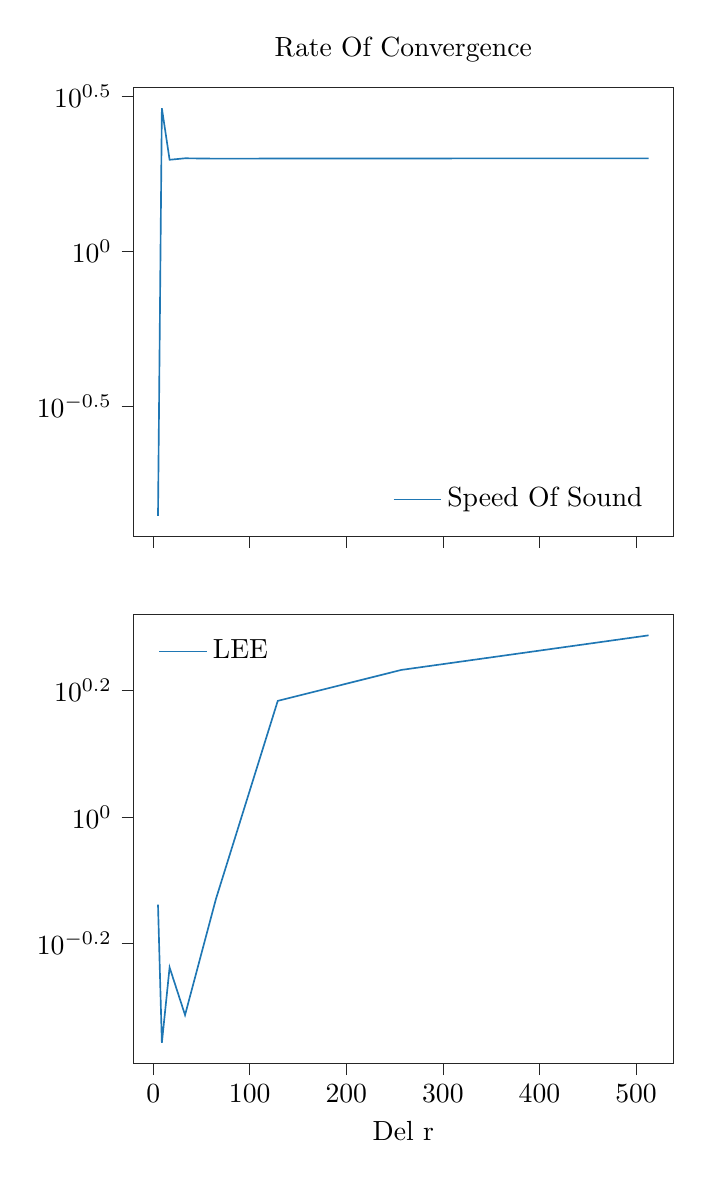
\begin{tikzpicture}

\definecolor{color0}{rgb}{0.12156862745098,0.466666666666667,0.705882352941177}

\begin{groupplot}[group style={group size=1 by 2}]
\nextgroupplot[
axis line style={white!15!black},
legend cell align={left},
legend style={
  fill opacity=0.8,
  draw opacity=1,
  text opacity=1,
  at={(0.97,0.03)},
  anchor=south east,
  draw=none
},
log basis y={10},
scaled x ticks=manual:{}{\pgfmathparse{#1}},
tick align=outside,
tick pos=left,
title={Rate Of Convergence},
x grid style={white!80!black},
xmin=-20.4, xmax=538.4,
xtick style={color=white!15!black},
xticklabels={},
y grid style={white!80!black},
ymin=0.120179448142703, ymax=3.37658389826634,
ymode=log,
ytick style={color=white!15!black}
]
\addplot [semithick, color0]
table {%
5 0.139854940165
9 2.901549198208
17 1.977988434508
33 1.999649604478
65 1.994368784807
129 1.995803507321
257 1.997560485834
513 1.998695137951
};
\addlegendentry{Speed Of Sound}

\nextgroupplot[
axis line style={white!15!black},
legend cell align={left},
legend style={
  fill opacity=0.8,
  draw opacity=1,
  text opacity=1,
  at={(0.03,0.97)},
  anchor=north west,
  draw=none
},
log basis y={10},
tick align=outside,
tick pos=left,
x grid style={white!80!black},
xlabel={Del r},
xmin=-20.4, xmax=538.4,
xtick style={color=white!15!black},
y grid style={white!80!black},
ymin=0.406988144058352, ymax=2.08856015532704,
ymode=log,
ytick style={color=white!15!black}
]
\addplot [semithick, color0]
table {%
5 0.72597886409
9 0.4383959579
17 0.577324517247
33 0.485337551867
65 0.741219384058
129 1.526486302345
257 1.708994456756
513 1.938930334674
};
\addlegendentry{LEE}
\end{groupplot}

\end{tikzpicture}
}
%     \end{center}
%     \caption{Rate of Convergence for the Speed of Sound Integration}
% \end{figure}

% \begin{figure}
%     \begin{center}
%         \scalebox{0.75}{% This file was created with tikzplotlib v0.9.12.
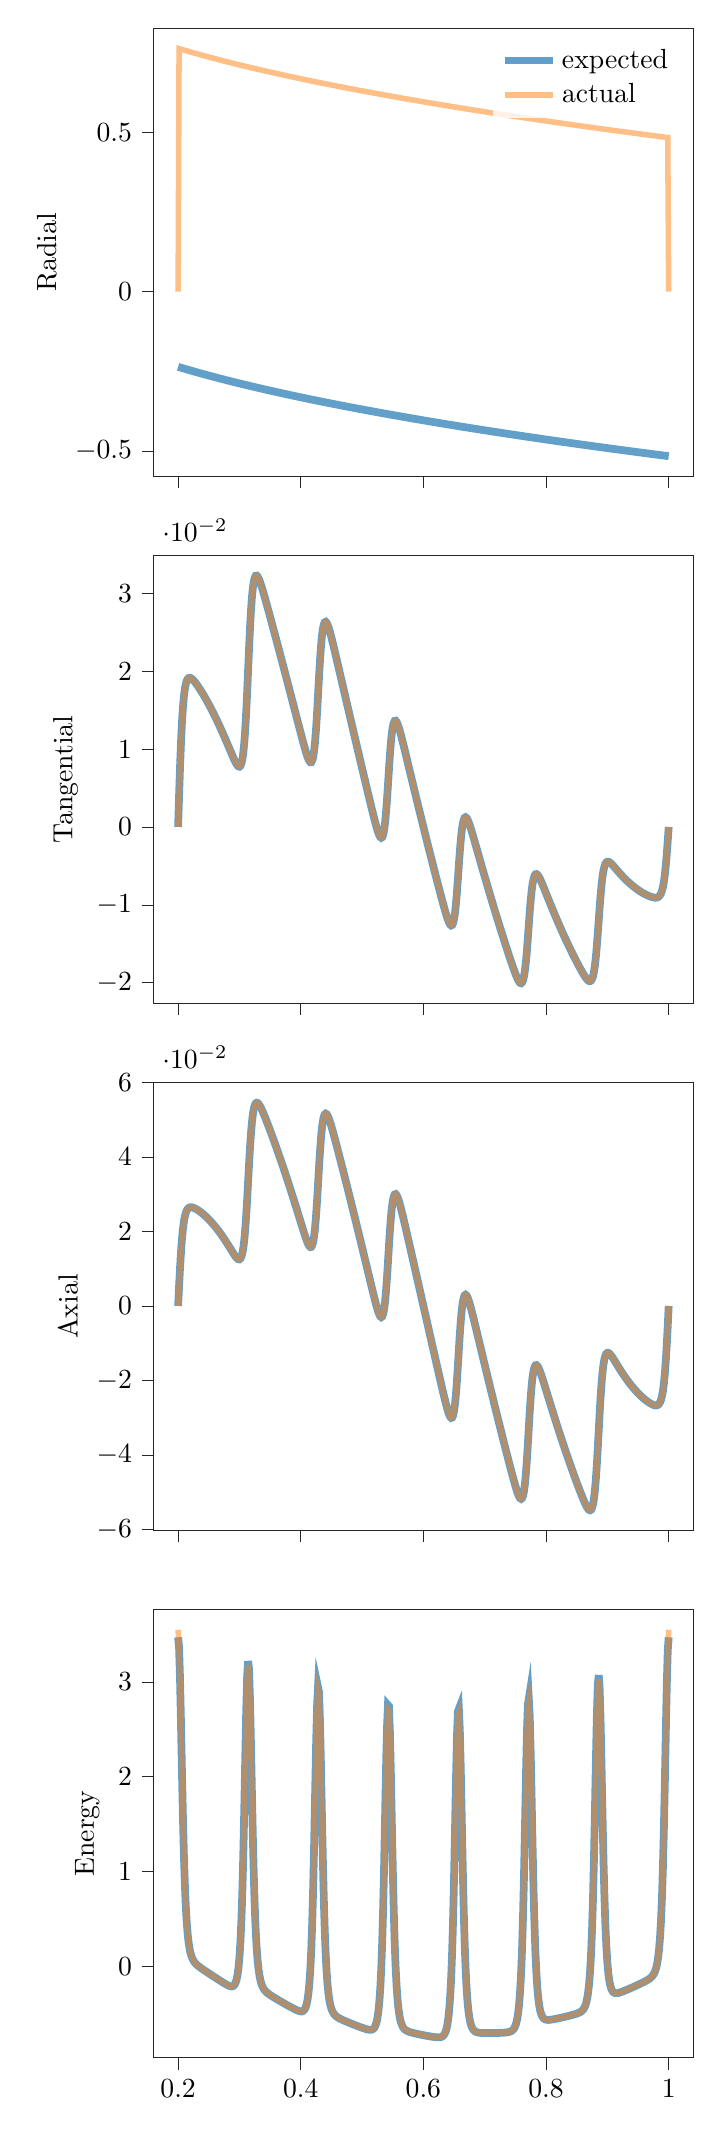
\begin{tikzpicture}

\definecolor{color0}{rgb}{0.12156862745098,0.466666666666667,0.705882352941177}
\definecolor{color1}{rgb}{1,0.498039215686275,0.0549019607843137}

\begin{groupplot}[group style={group size=1 by 4}]
\nextgroupplot[
axis line style={white!15!black},
legend cell align={left},
legend style={fill opacity=0.8, draw opacity=1, text opacity=1, draw=none},
scaled x ticks=manual:{}{\pgfmathparse{#1}},
tick align=outside,
tick pos=left,
x grid style={white!80!black},
xmin=0.16, xmax=1.04,
xtick style={color=white!15!black},
xticklabels={},
y grid style={white!80!black},
ylabel={Radial},
ymin=-0.580634431221742, ymax=0.826883665311966,
ytick style={color=white!15!black}
]
\addplot [line width=2.8pt, color0, opacity=0.7]
table {%
0.2 -0.236188215087245
0.2015625 -0.237094429985027
0.203125 -0.237997024650676
0.2046875 -0.238896040690986
0.20625 -0.239791518919342
0.2078125 -0.240683499376718
0.209375 -0.241572021351978
0.2109375 -0.242457123401487
0.2125 -0.243338843368075
0.2140625 -0.24421721839937
0.215625 -0.245092284965535
0.2171875 -0.245964078876424
0.21875 -0.246832635298181
0.2203125 -0.247697988769316
0.221875 -0.248560173216255
0.2234375 -0.249419221968412
0.225 -0.250275167772776
0.2265625 -0.251128042808052
0.228125 -0.251977878698352
0.2296875 -0.252824706526483
0.23125 -0.253668556846808
0.2328125 -0.254509459697732
0.234375 -0.255347444613805
0.2359375 -0.256182540637461
0.2375 -0.257014776330416
0.2390625 -0.257844179784714
0.240625 -0.258670778633468
0.2421875 -0.259494600061269
0.24375 -0.260315670814307
0.2453125 -0.261134017210191
0.246875 -0.261949665147495
0.2484375 -0.262762640115028
0.25 -0.263572967200845
0.2515625 -0.264380671100999
0.253125 -0.26518577612806
0.2546875 -0.265988306219384
0.25625 -0.266788284945164
0.2578125 -0.267585735516259
0.259375 -0.268380680791804
0.2609375 -0.269173143286619
0.2625 -0.269963145178419
0.2640625 -0.270750708314829
0.265625 -0.271535854220211
0.2671875 -0.272318604102318
0.26875 -0.27309897885876
0.2703125 -0.273876999083314
0.271875 -0.274652685072065
0.2734375 -0.275426056829385
0.275 -0.276197134073765
0.2765625 -0.27696593624349
0.278125 -0.27773248250218
0.2796875 -0.278496791744183
0.28125 -0.279258882599835
0.2828125 -0.280018773440588
0.284375 -0.280776482384016
0.2859375 -0.281532027298688
0.2875 -0.282285425808927
0.2890625 -0.283036695299453
0.290625 -0.283785852919915
0.2921875 -0.284532915589305
0.29375 -0.285277900000274
0.2953125 -0.286020822623344
0.296875 -0.286761699711017
0.2984375 -0.287500547301786
0.3 -0.288237381224057
0.3015625 -0.288972217099971
0.303125 -0.289705070349149
0.3046875 -0.290435956192335
0.30625 -0.291164889654967
0.3078125 -0.291891885570663
0.309375 -0.292616958584624
0.3109375 -0.293340123156963
0.3125 -0.294061393565959
0.3140625 -0.294780783911235
0.315625 -0.295498308116869
0.3171875 -0.296213979934431
0.31875 -0.296927812945959
0.3203125 -0.297639820566861
0.321875 -0.298350016048762
0.3234375 -0.299058412482284
0.325 -0.299765022799766
0.3265625 -0.300469859777923
0.328125 -0.301172936040457
0.3296875 -0.301874264060601
0.33125 -0.302573856163615
0.3328125 -0.303271724529225
0.334375 -0.303967881194017
0.3359375 -0.304662338053776
0.3375 -0.305355106865774
0.3390625 -0.306046199251015
0.340625 -0.306735626696434
0.3421875 -0.307423400557043
0.34375 -0.308109532058044
0.3453125 -0.30879403229689
0.346875 -0.309476912245306
0.3484375 -0.310158182751275
0.35 -0.310837854540973
0.3515625 -0.311515938220678
0.353125 -0.312192444278629
0.3546875 -0.312867383086854
0.35625 -0.313540764902963
0.3578125 -0.314212599871905
0.359375 -0.314882898027684
0.3609375 -0.315551669295051
0.3625 -0.316218923491157
0.3640625 -0.316884670327176
0.365625 -0.317548919409896
0.3671875 -0.31821168024328
0.36875 -0.318872962229997
0.3703125 -0.319532774672925
0.371875 -0.32019112677662
0.3734375 -0.320848027648768
0.375 -0.321503486301595
0.3765625 -0.322157511653269
0.378125 -0.322810112529253
0.3796875 -0.323461297663656
0.38125 -0.324111075700545
0.3828125 -0.324759455195235
0.384375 -0.325406444615556
0.3859375 -0.326052052343099
0.3875 -0.32669628667444
0.3890625 -0.327339155822334
0.390625 -0.327980667916897
0.3921875 -0.328620831006761
0.39375 -0.329259653060212
0.3953125 -0.329897141966303
0.396875 -0.330533305535951
0.3984375 -0.331168151503015
0.4 -0.331801687525351
0.4015625 -0.332433921185852
0.403125 -0.333064859993468
0.4046875 -0.333694511384213
0.40625 -0.334322882722144
0.4078125 -0.334949981300333
0.409375 -0.33557581434182
0.4109375 -0.336200389000547
0.4125 -0.336823712362276
0.4140625 -0.337445791445495
0.415625 -0.338066633202306
0.4171875 -0.338686244519297
0.41875 -0.339304632218404
0.4203125 -0.339921803057751
0.421875 -0.340537763732483
0.4234375 -0.341152520875584
0.425 -0.341766081058673
0.4265625 -0.342378450792803
0.428125 -0.34298963652923
0.4296875 -0.343599644660179
0.43125 -0.344208481519597
0.4328125 -0.344816153383891
0.434375 -0.345422666472654
0.4359375 -0.346028026949382
0.4375 -0.346632240922175
0.4390625 -0.347235314444434
0.440625 -0.347837253515539
0.4421875 -0.348438064081519
0.44375 -0.349037752035715
0.4453125 -0.349636323219425
0.446875 -0.350233783422549
0.4484375 -0.350830138384212
0.45 -0.351425393793387
0.4515625 -0.352019555289504
0.453125 -0.35261262846305
0.4546875 -0.353204618856157
0.45625 -0.35379553196319
0.4578125 -0.354385373231311
0.459375 -0.354974148061053
0.4609375 -0.355561861806866
0.4625 -0.356148519777669
0.4640625 -0.356734127237388
0.465625 -0.357318689405484
0.4671875 -0.357902211457477
0.46875 -0.358484698525463
0.4703125 -0.359066155698615
0.471875 -0.359646588023687
0.4734375 -0.360226000505503
0.475 -0.360804398107443
0.4765625 -0.36138178575192
0.478125 -0.361958168320851
0.4796875 -0.362533550656117
0.48125 -0.363107937560023
0.4828125 -0.363681333795748
0.484375 -0.364253744087784
0.4859375 -0.364825173122381
0.4875 -0.365395625547967
0.4890625 -0.365965105975582
0.490625 -0.366533618979289
0.4921875 -0.367101169096593
0.49375 -0.367667760828841
0.4953125 -0.368233398641626
0.496875 -0.368798086965183
0.4984375 -0.369361830194773
0.5 -0.369924632691076
0.5015625 -0.370486498780559
0.503125 -0.371047432755856
0.5046875 -0.371607438876135
0.50625 -0.372166521367457
0.5078125 -0.37272468442314
0.509375 -0.373281932204107
0.5109375 -0.373838268839234
0.5125 -0.374393698425696
0.5140625 -0.374948225029304
0.515625 -0.375501852684838
0.5171875 -0.376054585396377
0.51875 -0.376606427137625
0.5203125 -0.377157381852229
0.521875 -0.377707453454097
0.5234375 -0.378256645827708
0.525 -0.378804962828422
0.5265625 -0.379352408282782
0.528125 -0.379898985988813
0.5296875 -0.380444699716318
0.53125 -0.380989553207171
0.5328125 -0.381533550175603
0.534375 -0.382076694308485
0.5359375 -0.382618989265609
0.5375 -0.383160438679969
0.5390625 -0.383701046158024
0.540625 -0.384240815279977
0.5421875 -0.384779749600037
0.54375 -0.385317852646677
0.5453125 -0.385855127922903
0.546875 -0.386391578906499
0.5484375 -0.386927209050286
0.55 -0.387462021782371
0.5515625 -0.387996020506388
0.553125 -0.388529208601747
0.5546875 -0.389061589423867
0.55625 -0.389593166304419
0.5578125 -0.390123942551558
0.559375 -0.390653921450149
0.5609375 -0.391183106262003
0.5625 -0.391711500226093
0.5640625 -0.392239106558785
0.565625 -0.39276592845405
0.5671875 -0.393291969083685
0.56875 -0.393817231597525
0.5703125 -0.394341719123656
0.571875 -0.394865434768623
0.5734375 -0.395388381617635
0.575 -0.395910562734769
0.5765625 -0.396431981163175
0.578125 -0.396952639925267
0.5796875 -0.397472542022926
0.58125 -0.397991690437693
0.5828125 -0.398510088130957
0.584375 -0.399027738044147
0.5859375 -0.399544643098918
0.5875 -0.400060806197337
0.5890625 -0.400576230222064
0.590625 -0.401090918036533
0.5921875 -0.40160487248513
0.59375 -0.40211809639337
0.5953125 -0.402630592568069
0.596875 -0.403142363797518
0.5984375 -0.403653412851652
0.6 -0.404163742482217
0.6015625 -0.404673355422937
0.603125 -0.405182254389679
0.6046875 -0.405690442080614
0.60625 -0.406197921176374
0.6078125 -0.406704694340219
0.609375 -0.407210764218182
0.6109375 -0.407716133439235
0.6125 -0.408220804615433
0.6140625 -0.40872478034207
0.615625 -0.409228063197829
0.6171875 -0.409730655744924
0.61875 -0.410232560529254
0.6203125 -0.410733780080542
0.621875 -0.411234316912478
0.6234375 -0.411734173522863
0.625 -0.412233352393747
0.6265625 -0.412731855991566
0.628125 -0.413229686767279
0.6296875 -0.413726847156504
0.63125 -0.414223339579651
0.6328125 -0.414719166442052
0.634375 -0.415214330134094
0.6359375 -0.415708833031347
0.6375 -0.416202677494692
0.6390625 -0.416695865870445
0.640625 -0.417188400490485
0.6421875 -0.417680283672377
0.64375 -0.418171517719489
0.6453125 -0.41866210492112
0.646875 -0.419152047552616
0.6484375 -0.419641347875487
0.65 -0.420130008137525
0.6515625 -0.420618030572921
0.653125 -0.421105417402376
0.6546875 -0.421592170833217
0.65625 -0.422078293059509
0.6578125 -0.422563786262162
0.659375 -0.423048652609046
0.6609375 -0.423532894255094
0.6625 -0.424016513342412
0.6640625 -0.424499512000385
0.665625 -0.424981892345783
0.6671875 -0.42546365648286
0.66875 -0.425944806503462
0.6703125 -0.426425344487128
0.671875 -0.426905272501185
0.6734375 -0.427384592600856
0.675 -0.427863306829352
0.6765625 -0.428341417217973
0.678125 -0.428818925786201
0.6796875 -0.429295834541798
0.68125 -0.429772145480902
0.6828125 -0.430247860588116
0.684375 -0.430722981836605
0.6859375 -0.431197511188183
0.6875 -0.431671450593408
0.6890625 -0.432144801991668
0.690625 -0.432617567311275
0.6921875 -0.433089748469545
0.69375 -0.433561347372893
0.6953125 -0.434032365916913
0.696875 -0.434502805986467
0.6984375 -0.434972669455768
0.7 -0.435441958188463
0.7015625 -0.435910674037717
0.703125 -0.436378818846294
0.7046875 -0.436846394446638
0.70625 -0.437313402660953
0.7078125 -0.437779845301283
0.709375 -0.438245724169592
0.7109375 -0.438711041057837
0.7125 -0.439175797748052
0.7140625 -0.439639996012417
0.715625 -0.440103637613341
0.7171875 -0.440566724303531
0.71875 -0.441029257826069
0.7203125 -0.441491239914482
0.721875 -0.441952672292822
0.7234375 -0.442413556675729
0.725 -0.442873894768508
0.7265625 -0.443333688267199
0.728125 -0.443792938858643
0.7296875 -0.444251648220557
0.73125 -0.444709818021598
0.7328125 -0.445167449921432
0.734375 -0.445624545570804
0.7359375 -0.4460811066116
0.7375 -0.446537134676915
0.7390625 -0.44699263139112
0.740625 -0.447447598369924
0.7421875 -0.44790203722044
0.74375 -0.448355949541248
0.7453125 -0.448809336922456
0.746875 -0.449262200945766
0.7484375 -0.449714543184531
0.75 -0.450166365203821
0.7515625 -0.450617668560481
0.753125 -0.451068454803189
0.7546875 -0.451518725472518
0.75625 -0.451968482100998
0.7578125 -0.452417726213167
0.759375 -0.452866459325633
0.7609375 -0.453314682947133
0.7625 -0.453762398578583
0.7640625 -0.454209607713144
0.765625 -0.454656311836268
0.7671875 -0.455102512425759
0.76875 -0.455548210951827
0.7703125 -0.45599340887714
0.771875 -0.456438107656879
0.7734375 -0.456882308738792
0.775 -0.457326013563243
0.7765625 -0.45776922356327
0.778125 -0.458211940164633
0.7796875 -0.458654164785864
0.78125 -0.459095898838321
0.7828125 -0.459537143726238
0.784375 -0.459977900846772
0.7859375 -0.460418171590055
0.7875 -0.460857957339244
0.7890625 -0.461297259470565
0.790625 -0.461736079353366
0.7921875 -0.462174418350162
0.79375 -0.462612277816684
0.7953125 -0.463049659101923
0.796875 -0.46348656354818
0.7984375 -0.46392299249111
0.8 -0.464358947259767
0.8015625 -0.464794429176651
0.803125 -0.465229439557752
0.8046875 -0.465663979712595
0.80625 -0.466098050944283
0.8078125 -0.466531654549539
0.809375 -0.466964791818755
0.8109375 -0.46739746403603
0.8125 -0.467829672479213
0.8140625 -0.468261418419947
0.815625 -0.46869270312371
0.8171875 -0.469123527849855
0.81875 -0.469553893851653
0.8203125 -0.469983802376335
0.821875 -0.470413254665128
0.8234375 -0.470842251953298
0.825 -0.471270795470189
0.8265625 -0.471698886439265
0.828125 -0.472126526078144
0.8296875 -0.47255371559864
0.83125 -0.4729804562068
0.8328125 -0.473406749102945
0.834375 -0.473832595481702
0.8359375 -0.474257996532048
0.8375 -0.474682953437342
0.8390625 -0.475107467375364
0.840625 -0.475531539518351
0.8421875 -0.475955171033034
0.84375 -0.476378363080673
0.8453125 -0.476801116817092
0.846875 -0.477223433392715
0.8484375 -0.477645313952602
0.85 -0.47806675963648
0.8515625 -0.478487771578784
0.853125 -0.478908350908684
0.8546875 -0.479328498750123
0.85625 -0.479748216221848
0.8578125 -0.480167504437448
0.859375 -0.480586364505381
0.8609375 -0.481004797529009
0.8625 -0.481422804606634
0.8640625 -0.481840386831524
0.865625 -0.482257545291949
0.8671875 -0.482674281071213
0.86875 -0.483090595247683
0.8703125 -0.483506488894822
0.871875 -0.483921963081218
0.8734375 -0.484337018870616
0.875 -0.48475165732195
0.8765625 -0.485165879489369
0.878125 -0.485579686422273
0.8796875 -0.485993079165335
0.88125 -0.486406058758536
0.8828125 -0.486818626237195
0.884375 -0.487230782631993
0.8859375 -0.487642528969005
0.8875 -0.488053866269728
0.8890625 -0.488464795551111
0.890625 -0.488875317825579
0.8921875 -0.489285434101065
0.89375 -0.489695145381034
0.8953125 -0.490104452664514
0.896875 -0.490513356946122
0.8984375 -0.490921859216087
0.9 -0.491329960460285
0.9015625 -0.491737661660258
0.903125 -0.492144963793242
0.9046875 -0.492551867832198
0.90625 -0.49295837474583
0.9078125 -0.493364485498619
0.909375 -0.493770201050842
0.9109375 -0.4941755223586
0.9125 -0.494580450373845
0.9140625 -0.494984986044402
0.915625 -0.495389130313993
0.9171875 -0.495792884122266
0.91875 -0.496196248404815
0.9203125 -0.496599224093208
0.921875 -0.497001812115006
0.9234375 -0.497404013393793
0.925 -0.497805828849193
0.9265625 -0.498207259396901
0.928125 -0.4986083059487
0.9296875 -0.499008969412485
0.93125 -0.49940925069229
0.9328125 -0.499809150688306
0.934375 -0.500208670296908
0.9359375 -0.500607810410672
0.9375 -0.501006571918403
0.9390625 -0.501404955705154
0.940625 -0.501802962652246
0.9421875 -0.502200593637296
0.94375 -0.502597849534231
0.9453125 -0.502994731213317
0.946875 -0.503391239541173
0.9484375 -0.503787375380797
0.95 -0.504183139591585
0.9515625 -0.504578533029355
0.953125 -0.50497355654636
0.9546875 -0.505368210991319
0.95625 -0.505762497209427
0.9578125 -0.506156416042384
0.959375 -0.506549968328409
0.9609375 -0.506943154902262
0.9625 -0.507335976595265
0.9640625 -0.507728434235319
0.965625 -0.508120528646926
0.9671875 -0.508512260651207
0.96875 -0.50890363106592
0.9703125 -0.509294640705482
0.971875 -0.509685290380987
0.9734375 -0.510075580900223
0.975 -0.510465513067691
0.9765625 -0.510855087684625
0.978125 -0.51124430554901
0.9796875 -0.511633167455601
0.98125 -0.512021674195937
0.9828125 -0.512409826558365
0.984375 -0.512797625328053
0.9859375 -0.51318507128701
0.9875 -0.513572165214104
0.9890625 -0.513958907885077
0.990625 -0.514345300072566
0.9921875 -0.514731342546115
0.99375 -0.5151170360722
0.9953125 -0.515502381414237
0.996875 -0.515887379332605
0.9984375 -0.516272030584661
1 -0.516656335924755
};
\addlegendentry{expected}
\addplot [line width=2pt, color1, opacity=0.5]
table {%
0.2 0
0.2015625 0.762905570014979
0.203125 0.762002975349326
0.2046875 0.761103959309031
0.20625 0.760208481080657
0.2078125 0.759316500623273
0.209375 0.758427978648015
0.2109375 0.757542876598514
0.2125 0.75666115663194
0.2140625 0.755782781600633
0.215625 0.754907715034465
0.2171875 0.754035921123574
0.21875 0.753167364701831
0.2203125 0.752302011230702
0.221875 0.751439826783741
0.2234375 0.750580778031578
0.225 0.749724832227216
0.2265625 0.748871957191959
0.228125 0.74802212130165
0.2296875 0.747175293473507
0.23125 0.746331443153197
0.2328125 0.745490540302271
0.234375 0.744652555386203
0.2359375 0.743817459362552
0.2375 0.742985223669582
0.2390625 0.742155820215276
0.240625 0.741329221366527
0.2421875 0.740505399938733
0.24375 0.739684329185698
0.2453125 0.738865982789807
0.246875 0.738050334852504
0.2484375 0.737237359884972
0.25 0.736427032799163
0.2515625 0.735619328899006
0.253125 0.734814223871926
0.2546875 0.734011693780612
0.25625 0.733211715054836
0.2578125 0.732414264483744
0.259375 0.731619319208207
0.2609375 0.730826856713382
0.2625 0.730036854821574
0.2640625 0.729249291685164
0.265625 0.728464145779775
0.2671875 0.72768139589769
0.26875 0.726901021141234
0.2703125 0.726123000916683
0.271875 0.72534731492793
0.2734375 0.724573943170604
0.275 0.723802865926245
0.2765625 0.723034063756518
0.278125 0.722267517497809
0.2796875 0.721503208255811
0.28125 0.720741117400159
0.2828125 0.719981226559426
0.284375 0.719223517615976
0.2859375 0.718467972701315
0.2875 0.717714574191078
0.2890625 0.716963304700549
0.290625 0.716214147080095
0.2921875 0.715467084410694
0.29375 0.714722099999729
0.2953125 0.713979177376658
0.296875 0.713238300288971
0.2984375 0.712499452698225
0.3 0.711762618775939
0.3015625 0.711027782900029
0.303125 0.710294929650857
0.3046875 0.709564043807653
0.30625 0.708835110345035
0.3078125 0.708108114429326
0.309375 0.70738304141538
0.3109375 0.706659876843034
0.3125 0.705938606434039
0.3140625 0.705219216088778
0.315625 0.704501691883141
0.3171875 0.703786020065575
0.31875 0.703072187054048
0.3203125 0.702360179433135
0.321875 0.701649983951242
0.3234375 0.700941587517708
0.325 0.700234977200218
0.3265625 0.699530140222066
0.328125 0.698827063959563
0.3296875 0.698125735939414
0.33125 0.697426143836385
0.3328125 0.696728275470754
0.334375 0.696032118805974
0.3359375 0.695337661946247
0.3375 0.694644893134239
0.3390625 0.693953800748989
0.340625 0.693264373303542
0.3421875 0.692576599442958
0.34375 0.691890467941967
0.3453125 0.691205967703126
0.346875 0.690523087754702
0.3484375 0.68984181724873
0.35 0.689162145459022
0.3515625 0.688484061779313
0.353125 0.687807555721392
0.3546875 0.687132616913136
0.35625 0.686459235097043
0.3578125 0.685787400128092
0.359375 0.685117101972317
0.3609375 0.684448330704967
0.3625 0.68378107650884
0.3640625 0.683115329672813
0.365625 0.682451080590099
0.3671875 0.681788319756713
0.36875 0.681127037770025
0.3703125 0.680467225327067
0.371875 0.679808873223376
0.3734375 0.679151972351235
0.375 0.678496513698398
0.3765625 0.677842488346741
0.378125 0.67718988747075
0.3796875 0.676538702336341
0.38125 0.675888924299443
0.3828125 0.675240544804772
0.384375 0.674593555384462
0.3859375 0.673947947656902
0.3875 0.673303713325563
0.3890625 0.67266084417767
0.390625 0.672019332083103
0.3921875 0.671379168993255
0.39375 0.670740346939784
0.3953125 0.670102858033697
0.396875 0.669466694464035
0.3984375 0.668831848496971
0.4 0.668198312474658
0.4015625 0.667566078814136
0.403125 0.66693514000654
0.4046875 0.666305488615791
0.40625 0.665677117277831
0.4078125 0.665050018699688
0.409375 0.664424185658167
0.4109375 0.663799610999444
0.4125 0.663176287637697
0.4140625 0.662554208554504
0.415625 0.661933366797697
0.4171875 0.661313755480709
0.41875 0.660695367781596
0.4203125 0.660078196942237
0.421875 0.659462236267508
0.4234375 0.658847479124418
0.425 0.658233918941338
0.4265625 0.657621549207203
0.428125 0.657010363470761
0.4296875 0.656400355339805
0.43125 0.655791518480399
0.4328125 0.655183846616101
0.434375 0.654577333527339
0.4359375 0.653971973050602
0.4375 0.653367759077845
0.4390625 0.652764685555567
0.440625 0.652162746484439
0.4421875 0.651561935918476
0.44375 0.650962247964287
0.4453125 0.650363676780565
0.446875 0.649766216577475
0.4484375 0.649169861615778
0.45 0.648574606206619
0.4515625 0.647980444710498
0.453125 0.647387371536958
0.4546875 0.64679538114386
0.45625 0.646204468036817
0.4578125 0.645614626768701
0.459375 0.645025851938925
0.4609375 0.644438138193131
0.4625 0.643851480222324
0.4640625 0.643265872762615
0.465625 0.642681310594508
0.4671875 0.642097788542515
0.46875 0.641515301474534
0.4703125 0.640933844301415
0.471875 0.640353411976296
0.4734375 0.639773999494491
0.475 0.639195601892567
0.4765625 0.638618214248091
0.478125 0.638041831679161
0.4796875 0.637466449343894
0.48125 0.636892062439966
0.4828125 0.636318666204232
0.484375 0.635746255912217
0.4859375 0.635174826877645
0.4875 0.634604374452014
0.4890625 0.63403489402442
0.490625 0.633466381020696
0.4921875 0.632898830903379
0.49375 0.632332239171163
0.4953125 0.631766601358382
0.496875 0.631201913034811
0.4984375 0.630638169805223
0.5 0.630075367308912
0.5015625 0.629513501219449
0.503125 0.628952567244127
0.5046875 0.62839256112386
0.50625 0.627833478632539
0.5078125 0.627275315576845
0.509375 0.626718067795892
0.5109375 0.626161731160764
0.5125 0.625606301574322
0.5140625 0.6250517749707
0.515625 0.624498147315144
0.5171875 0.623945414603625
0.51875 0.623393572862355
0.5203125 0.622842618147786
0.521875 0.622292546545935
0.5234375 0.62174335417226
0.525 0.621195037171603
0.5265625 0.620647591717173
0.528125 0.620101014011198
0.5296875 0.619555300283679
0.53125 0.619010446792806
0.5328125 0.618466449824396
0.534375 0.617923305691491
0.5359375 0.617381010734391
0.5375 0.616839561320034
0.5390625 0.616298953841955
0.540625 0.615759184720034
0.5421875 0.615220250399929
0.54375 0.614682147353335
0.5453125 0.614144872077105
0.546875 0.613608421093467
0.5484375 0.613072790949715
0.55 0.612537978217617
0.5515625 0.612003979493608
0.553125 0.611470791398261
0.5546875 0.610938410576132
0.55625 0.610406833695592
0.5578125 0.609876057448432
0.559375 0.609346078549862
0.5609375 0.608816893738009
0.5625 0.608288499773899
0.5640625 0.60776089344121
0.565625 0.607234071545932
0.5671875 0.606708030916337
0.56875 0.606182768402476
0.5703125 0.605658280876305
0.571875 0.605134565231381
0.5734375 0.60461161838235
0.575 0.60408943726523
0.5765625 0.603568018836825
0.578125 0.603047360074733
0.5796875 0.602527457977075
0.58125 0.602008309562294
0.5828125 0.601489911869066
0.584375 0.60097226195586
0.5859375 0.600455356901058
0.5875 0.599939193802683
0.5890625 0.599423769777914
0.590625 0.598909081963484
0.5921875 0.598395127514891
0.59375 0.597881903606613
0.5953125 0.597369407431941
0.596875 0.596857636202443
0.5984375 0.596346587148361
0.6 0.595836257517789
0.6015625 0.595326644577064
0.603125 0.594817745610342
0.6046875 0.594309557919374
0.60625 0.593802078823643
0.6078125 0.593295305659808
0.609375 0.592789235781801
0.6109375 0.592283866560777
0.6125 0.591779195384547
0.6140625 0.591275219657945
0.615625 0.590771936802184
0.6171875 0.590269344255042
0.61875 0.589767439470748
0.6203125 0.589266219919423
0.621875 0.58876568308753
0.6234375 0.588265826477169
0.625 0.587766647606237
0.6265625 0.587268144008462
0.628125 0.586770313232719
0.6296875 0.586273152843518
0.63125 0.585776660420379
0.6328125 0.585280833557938
0.634375 0.584785669865894
0.6359375 0.584291166968612
0.6375 0.583797322505319
0.6390625 0.583304134129577
0.640625 0.58281159950949
0.6421875 0.582319716327632
0.64375 0.5818284822805
0.6453125 0.581337895078889
0.646875 0.580847952447385
0.6484375 0.580358652124495
0.65 0.57986999186248
0.6515625 0.579381969427047
0.653125 0.578894582597627
0.6546875 0.578407829166792
0.65625 0.577921706940494
0.6578125 0.57743621373784
0.659375 0.576951347390931
0.6609375 0.576467105744911
0.6625 0.575983486657606
0.6640625 0.575500487999598
0.665625 0.57501810765423
0.6671875 0.574536343517124
0.66875 0.574055193496548
0.6703125 0.573574655512885
0.671875 0.573094727498791
0.6734375 0.572615407399169
0.675 0.572136693170606
0.6765625 0.57165858278205
0.678125 0.571181074213825
0.6796875 0.570704165458188
0.68125 0.570227854519104
0.6828125 0.569752139411847
0.684375 0.569277018163433
0.6859375 0.568802488811826
0.6875 0.56832854940658
0.6890625 0.567855198008331
0.690625 0.567382432688717
0.6921875 0.566910251530487
0.69375 0.566438652627113
0.6953125 0.565967634083059
0.696875 0.565497194013531
0.6984375 0.565027330544225
0.7 0.564558041811551
0.7015625 0.5640893259623
0.703125 0.563621181153721
0.7046875 0.563153605553353
0.70625 0.562686597338981
0.7078125 0.562220154698736
0.709375 0.561754275830424
0.7109375 0.5612889589422
0.7125 0.560824202251965
0.7140625 0.560360003987526
0.715625 0.559896362386667
0.7171875 0.559433275696477
0.71875 0.55897074217394
0.7203125 0.55850876008553
0.721875 0.558047327707115
0.7234375 0.557586443324283
0.725 0.557126105231504
0.7265625 0.556666311732826
0.728125 0.556207061141365
0.7296875 0.5557483517794
0.73125 0.555290181978421
0.7328125 0.554832550078601
0.734375 0.554375454429206
0.7359375 0.553918893388427
0.7375 0.553462865323027
0.7390625 0.553007368608888
0.740625 0.552552401630095
0.7421875 0.55209796277957
0.74375 0.551644050458762
0.7453125 0.551190663077492
0.746875 0.550737799054246
0.7484375 0.550285456815487
0.75 0.549833634796201
0.7515625 0.549382331439531
0.753125 0.548931545196765
0.7546875 0.548481274527518
0.75625 0.548031517899005
0.7578125 0.54758227378683
0.759375 0.54713354067438
0.7609375 0.546685317052791
0.7625 0.546237601421439
0.7640625 0.545790392286847
0.765625 0.545343688163754
0.7671875 0.544897487574261
0.76875 0.544451789048097
0.7703125 0.544006591122866
0.771875 0.543561892343121
0.7734375 0.54311769126123
0.775 0.542673986436782
0.7765625 0.542230776436682
0.778125 0.541788059835397
0.7796875 0.541345835214173
0.78125 0.540904101161672
0.7828125 0.540462856273748
0.784375 0.540022099153148
0.7859375 0.539581828409951
0.7875 0.539142042660757
0.7890625 0.538702740529445
0.790625 0.538263920646656
0.7921875 0.537825581649784
0.79375 0.537387722183354
0.7953125 0.536950340898073
0.796875 0.536513436451841
0.7984375 0.536077007508894
0.8 0.535641052740189
0.8015625 0.535205570823365
0.803125 0.534770560442268
0.8046875 0.534336020287455
0.80625 0.53390194905576
0.8078125 0.53346834545043
0.809375 0.533035208181303
0.8109375 0.532602535963974
0.8125 0.532170327520802
0.8140625 0.531738581580058
0.815625 0.53130729687625
0.8171875 0.53087647215014
0.81875 0.530446106148361
0.8203125 0.530016197623681
0.821875 0.529586745334896
0.8234375 0.529157748046643
0.825 0.52872920452981
0.8265625 0.528301113560758
0.828125 0.527873473921872
0.8296875 0.527446284401393
0.83125 0.527019543793116
0.8328125 0.526593250897093
0.834375 0.526167404518333
0.8359375 0.525742003467982
0.8375 0.525317046562705
0.8390625 0.524892532624548
0.840625 0.524468460481699
0.8421875 0.524044828966964
0.84375 0.523621636919344
0.8453125 0.523198883182957
0.846875 0.522776566607192
0.8484375 0.522354686047464
0.85 0.52193324036358
0.8515625 0.521512228421201
0.853125 0.521091649091332
0.8546875 0.520671501249794
0.85625 0.52025178377815
0.8578125 0.519832495562525
0.859375 0.519413635494672
0.8609375 0.518995202471004
0.8625 0.51857719539332
0.8640625 0.518159613168535
0.865625 0.51774245470807
0.8671875 0.517325718928802
0.86875 0.516909404752326
0.8703125 0.516493511105111
0.871875 0.516078036918799
0.8734375 0.515662981129367
0.875 0.515248342678078
0.8765625 0.514834120510628
0.878125 0.514420313577702
0.8796875 0.514006920834703
0.88125 0.513593941241481
0.8828125 0.513181373762777
0.884375 0.512769217368046
0.8859375 0.512357471030938
0.8875 0.511946133730333
0.8890625 0.511535204448876
0.890625 0.51112468217444
0.8921875 0.510714565898937
0.89375 0.510304854618866
0.8953125 0.509895547335503
0.896875 0.50948664305389
0.8984375 0.509078140783956
0.9 0.508670039539723
0.9015625 0.508262338339691
0.903125 0.507855036206792
0.9046875 0.507448132167781
0.90625 0.507041625254189
0.9078125 0.506635514501354
0.909375 0.506229798949093
0.9109375 0.505824477641425
0.9125 0.505419549626197
0.9140625 0.505015013955628
0.915625 0.504610869686033
0.9171875 0.504207115877691
0.91875 0.5038037515952
0.9203125 0.503400775906812
0.921875 0.502998187885041
0.9234375 0.50259598660621
0.925 0.502194171150776
0.9265625 0.501792740603065
0.928125 0.501391694051335
0.9296875 0.500991030587485
0.93125 0.500590749307733
0.9328125 0.500190849311636
0.934375 0.499791329703129
0.9359375 0.499392189589344
0.9375 0.498993428081619
0.9390625 0.498595044294873
0.940625 0.498197037347651
0.9421875 0.497799406362702
0.94375 0.497402150465746
0.9453125 0.497005268786708
0.946875 0.496608760458813
0.9484375 0.496212624619133
0.95 0.495816860408439
0.9515625 0.495421466970697
0.953125 0.495026443453682
0.9546875 0.494631789008693
0.95625 0.494237502790483
0.9578125 0.493843583957613
0.959375 0.493450031671614
0.9609375 0.493056845097769
0.9625 0.492664023404714
0.9640625 0.492271565764597
0.965625 0.491879471353087
0.9671875 0.491487739348827
0.96875 0.491096368934094
0.9703125 0.490705359294523
0.971875 0.490314709618971
0.9734375 0.489924419099822
0.975 0.489534486932314
0.9765625 0.489144912315382
0.978125 0.488755694450972
0.9796875 0.488366832544372
0.98125 0.48797832580405
0.9828125 0.487590173441617
0.984375 0.48720237467198
0.9859375 0.486814928713002
0.9875 0.486427834785829
0.9890625 0.486041092114902
0.990625 0.485654699927466
0.9921875 0.485268657453886
0.99375 0.484882963927831
0.9953125 0.484497618585678
0.996875 0.484112620667446
0.9984375 0.483727969415383
1 0
};
\addlegendentry{actual}

\nextgroupplot[
axis line style={white!15!black},
scaled x ticks=manual:{}{\pgfmathparse{#1}},
tick align=outside,
tick pos=left,
x grid style={white!80!black},
xmin=0.16, xmax=1.04,
xtick style={color=white!15!black},
xticklabels={},
y grid style={white!80!black},
ylabel={Tangential},
ymin=-0.022688466064242, ymax=0.0348875014200262,
ytick style={color=white!15!black}
]
\addplot [line width=2.8pt, color0, opacity=0.7]
table {%
0.2 6.26089675733245e-17
0.2015625 0.0040093644295142
0.203125 0.00769462767530956
0.2046875 0.0108505375653979
0.20625 0.0133876669213113
0.2078125 0.0153194273291617
0.209375 0.0167232174727022
0.2109375 0.0177012227162371
0.2125 0.0183538328072859
0.2140625 0.0187666650027565
0.215625 0.0190069721090554
0.2171875 0.0191249270945586
0.21875 0.0191567315076122
0.2203125 0.0191279393958234
0.221875 0.0190563304318992
0.2234375 0.0189541594255005
0.225 0.0188298232995375
0.2265625 0.0186890560333773
0.228125 0.01853576748201
0.2296875 0.0183726242818433
0.23125 0.0182014485815553
0.2328125 0.0180234901208821
0.234375 0.0178396111600897
0.2359375 0.0176504118468312
0.2375 0.0174563150571966
0.2390625 0.0172576237459368
0.240625 0.0170545596855667
0.2421875 0.0168472896228422
0.24375 0.0166359429361802
0.2453125 0.0164206235560631
0.246875 0.0162014180149103
0.2484375 0.0159784008871327
0.25 0.0157516384709559
0.2515625 0.0155211912876639
0.253125 0.0152871157882061
0.2546875 0.0150494655325801
0.25625 0.0148082920245369
0.2578125 0.0145636453299477
0.259375 0.0143155745730844
0.2609375 0.0140641283857288
0.2625 0.0138093553763634
0.2640625 0.0135513046894542
0.265625 0.0132900267383802
0.2671875 0.0130255742219055
0.26875 0.0127580035772311
0.2703125 0.0124873770891219
0.271875 0.0122137659744893
0.2734375 0.0119372549102449
0.275 0.0116579486916993
0.2765625 0.0113759820323395
0.278125 0.0110915339920198
0.2796875 0.0108048492203014
0.28125 0.010516269227749
0.2828125 0.0102262783986044
0.284375 0.00993557164414853
0.2859375 0.00964515376128809
0.2875 0.00935648510294041
0.2890625 0.00907169459402506
0.290625 0.00879389002250065
0.2921875 0.00852760740540316
0.29375 0.00827945608070446
0.2953125 0.00805903248981462
0.296875 0.0078801881118025
0.2984375 0.00776273212358575
0.3 0.00773459703585583
0.3015625 0.0078343368268133
0.303125 0.00811346254468615
0.3046875 0.00863742308901203
0.30625 0.00948295765296642
0.3078125 0.0107284129330198
0.309375 0.0124336873004632
0.3109375 0.0146101255134405
0.3125 0.0171896347361232
0.3140625 0.0200124812182658
0.315625 0.0228522094724566
0.3171875 0.0254749051650816
0.31875 0.027702929311296
0.3203125 0.0294492457319962
0.321875 0.030712377360444
0.3234375 0.0315472831556359
0.325 0.0320332515916637
0.3265625 0.0322509207422946
0.328125 0.0322703817414986
0.3296875 0.0321473493460769
0.33125 0.0319237185167818
0.3328125 0.0316298825707061
0.334375 0.0312873767004808
0.3359375 0.0309112228494524
0.3375 0.0305117914623062
0.3390625 0.0300961931261663
0.340625 0.0296692820021403
0.3421875 0.0292343631813262
0.34375 0.0287936841163858
0.3453125 0.0283487727958455
0.346875 0.0279006689879367
0.3484375 0.0274500816995033
0.35 0.0269974960907574
0.3515625 0.0265432459331746
0.353125 0.0260875626531882
0.3546875 0.0256306084998219
0.35625 0.025172498963244
0.3578125 0.0247133179228166
0.359375 0.0242531278810135
0.3609375 0.0237919768777892
0.3625 0.0233299031638948
0.3640625 0.0228669383625355
0.365625 0.0224031096129836
0.3671875 0.0219384410308239
0.36875 0.0214729547127507
0.3703125 0.021006671442639
0.371875 0.0205396112088758
0.3734375 0.0200717936133598
0.375 0.0196032382355286
0.3765625 0.0191339650075702
0.378125 0.0186639946584707
0.3796875 0.0181933492949301
0.38125 0.0177220532080163
0.3828125 0.0172501340288781
0.384375 0.0167776244101624
0.3859375 0.0163045644900979
0.3875 0.0158310055157451
0.3890625 0.0153570151788378
0.390625 0.0148826854787393
0.3921875 0.0144081443116613
0.39375 0.0139335725509705
0.3953125 0.0134592292138015
0.396875 0.0129854885250646
0.3984375 0.0125128944635745
0.4 0.0120422409479246
0.4015625 0.0115746895206178
0.403125 0.0111119416434845
0.4046875 0.0106564900261307
0.40625 0.0102119832394238
0.4078125 0.00978375033680173
0.409375 0.00937954631432416
0.4109375 0.00901059113885203
0.4125 0.00869297454816854
0.4140625 0.00844946277205094
0.415625 0.00831162548851714
0.4171875 0.0083219214973262
0.41875 0.00853483105914595
0.4203125 0.00901523596748847
0.421875 0.00983123479805171
0.4234375 0.0110383712347028
0.425 0.0126547936961699
0.4265625 0.0146339188012792
0.428125 0.016850303127935
0.4296875 0.0191157599019048
0.43125 0.0212269346404409
0.4328125 0.0230214549724869
0.434375 0.0244123192221854
0.4359375 0.0253881962812026
0.4375 0.0259903888639087
0.4390625 0.0262848562196565
0.440625 0.0263411094887041
0.4421875 0.026220712957533
0.44375 0.0259731664625627
0.4453125 0.0256359699793578
0.446875 0.025236465778883
0.4484375 0.0247940948961932
0.45 0.0243224517282896
0.4515625 0.0238309373668446
0.453125 0.0233260053331039
0.4546875 0.0228120644214886
0.45625 0.0222921173724061
0.4578125 0.021768205691918
0.459375 0.02124171631775
0.4609375 0.0207135916193097
0.4625 0.0201844725575238
0.4640625 0.0196547959855804
0.465625 0.0191248606474091
0.4671875 0.0185948718833709
0.46875 0.0180649718853077
0.4703125 0.0175352601597348
0.471875 0.017005807363078
0.4734375 0.0164766646539454
0.475 0.0159478700150576
0.4765625 0.015419452527977
0.478125 0.0148914352659414
0.4796875 0.0143638372552621
0.48125 0.0138366748107879
0.4828125 0.013309962453461
0.484375 0.0127837135528631
0.4859375 0.0122579407947688
0.4875 0.0117326565463995
0.4890625 0.0112078731760512
0.490625 0.0106836033765474
0.4921875 0.0101598605424002
0.49375 0.0096366592586911
0.4953125 0.00911401597673386
0.496875 0.00859194998016401
0.4984375 0.00807048478956311
0.5 0.00754965022087908
0.5015625 0.00702948541298558
0.503125 0.00651004328797954
0.5046875 0.00599139712676216
0.50625 0.00547365026517371
0.5078125 0.00495695039089534
0.509375 0.00444151061902514
0.5109375 0.00392764054666539
0.5125 0.00341579197989458
0.5140625 0.00290662619536604
0.515625 0.00240111272449535
0.5171875 0.00190067409838392
0.51875 0.00140739720751245
0.5203125 0.000924340346963263
0.521875 0.000455975822058038
0.5234375 8.82051131330594e-06
0.525 -0.000407681872267704
0.5265625 -0.000779960878306466
0.528125 -0.00108876115904328
0.5296875 -0.00130727580146219
0.53125 -0.00139924302213281
0.5328125 -0.00131772704048192
0.534375 -0.0010060524851426
0.5359375 -0.000403280243381223
0.5375 0.00054300579551625
0.5390625 0.00185560413662024
0.540625 0.00350298210735037
0.5421875 0.00538389138385692
0.54375 0.00733716317347289
0.5453125 0.00918071743882227
0.546875 0.0107621730280265
0.5484375 0.0119934979315223
0.55 0.0128555241869398
0.5515625 0.0133794996926745
0.553125 0.0136220281780246
0.5546875 0.0136451182160257
0.55625 0.0135047797504287
0.5578125 0.0132465785095164
0.559375 0.0129052948253496
0.5609375 0.0125064153417437
0.5625 0.0120681236756729
0.5640625 0.0116031651004332
0.565625 0.0111203681592227
0.5671875 0.0106258004250635
0.56875 0.0101236103708655
0.5703125 0.00961662489567099
0.571875 0.00910676644015768
0.5734375 0.00859534102222019
0.575 0.0080832357169143
0.5765625 0.0075710534056698
0.578125 0.00705920442818126
0.5796875 0.006547968787341
0.58125 0.00603753830745461
0.5828125 0.00552804517858764
0.584375 0.00501958127091988
0.5859375 0.00451221119837416
0.5875 0.00400598115250575
0.5890625 0.00350092487597989
0.590625 0.00299706770279318
0.5921875 0.00249442929288506
0.59375 0.00199302548620128
0.5953125 0.00149286956450235
0.596875 0.000993973117151661
0.5984375 0.00049634664552443
0.6 2.17374337465462e-16
0.6015625 -0.000495057282574519
0.603125 -0.000988815688609672
0.6046875 -0.00148126543974945
0.60625 -0.00197239616264465
0.6078125 -0.00246219646565685
0.609375 -0.00295065335740226
0.6109375 -0.00343775141780874
0.6125 -0.00392347159440462
0.6140625 -0.00440778943909279
0.615625 -0.00489067251488311
0.6171875 -0.00537207657488834
0.61875 -0.00585193992797981
0.6203125 -0.00633017512838201
0.621875 -0.00680665671847151
0.6234375 -0.00728120315433573
0.625 -0.00775355016422241
0.6265625 -0.00822331150468559
0.628125 -0.00868992120990604
0.6296875 -0.00915254873117435
0.63125 -0.00960997451227245
0.6328125 -0.0100604081472421
0.634375 -0.0105012239124341
0.6359375 -0.0109285789256572
0.6375 -0.0113368678977699
0.6390625 -0.0117179576209475
0.640625 -0.0120601403157992
0.6421875 -0.0123467626682304
0.64375 -0.012554557841071
0.6453125 -0.0126518874136392
0.646875 -0.0125974731117139
0.6484375 -0.0123408400525841
0.65 -0.0118265301005737
0.6515625 -0.0110046344427443
0.653125 -0.00984898365104375
0.6546875 -0.00837971461131486
0.65625 -0.00667946070595
0.6578125 -0.00488843183868427
0.659375 -0.00317227382369336
0.6609375 -0.00167601136926057
0.6625 -0.000489163858625337
0.6640625 0.000362338502915954
0.665625 0.000901540363305858
0.6671875 0.00117773161538795
0.66875 0.00124729645236182
0.6703125 0.00116224778757102
0.671875 0.000965424651850844
0.6734375 0.000689782413075122
0.675 0.000359594870409553
0.6765625 -7.75957397983405e-06
0.678125 -0.000400071103923686
0.6796875 -0.00080886815732932
0.68125 -0.0012283218069492
0.6828125 -0.00165444355242926
0.684375 -0.00208451403108226
0.6859375 -0.0025166833173856
0.6875 -0.00294969448131619
0.6890625 -0.00338269384542068
0.690625 -0.00381510140810586
0.6921875 -0.00424652265435411
0.69375 -0.00467668867095451
0.6953125 -0.00510541554400499
0.696875 -0.00553257685822542
0.6984375 -0.00595808508301753
0.7 -0.00638187897906561
0.7015625 -0.00680391508028034
0.703125 -0.00722416193261498
0.7046875 -0.00764259619675286
0.70625 -0.00805920000999748
0.7078125 -0.00847395919781088
0.709375 -0.00888686205723674
0.7109375 -0.00929789852322476
0.7125 -0.00970705958834712
0.7140625 -0.010114336885778
0.715625 -0.0105197223708035
0.7171875 -0.0109232080514751
0.71875 -0.0113247857267171
0.7203125 -0.0117244466914398
0.721875 -0.0121221813632042
0.7234375 -0.0125179787729782
0.725 -0.0129118258416738
0.7265625 -0.0133037063312716
0.728125 -0.0136935993093882
0.7296875 -0.0140814768914689
0.73125 -0.0144673009139997
0.7328125 -0.0148510180283338
0.734375 -0.0152325524630741
0.7359375 -0.015611795347008
0.7375 -0.0159885889611715
0.7390625 -0.0163627035206381
0.740625 -0.01673380296334
0.7421875 -0.0171013945878732
0.74375 -0.0174647550180148
0.7453125 -0.0178228215901128
0.746875 -0.0181740335028364
0.7484375 -0.0185161005545059
0.75 -0.0188456687652717
0.7515625 -0.0191578419056332
0.753125 -0.0194455076341762
0.7546875 -0.0196984116809731
0.75625 -0.0199019355785704
0.7578125 -0.0200355888047808
0.759375 -0.0200713731722096
0.7609375 -0.0199724905674741
0.7625 -0.0196934207092211
0.7640625 -0.0191831592941205
0.765625 -0.0183939647120256
0.7671875 -0.0172971755860515
0.76875 -0.0159039095404667
0.7703125 -0.0142817167562052
0.771875 -0.0125535576972532
0.7734375 -0.0108714631894122
0.775 -0.00937451168061549
0.7765625 -0.00815385069298273
0.778125 -0.00724148980135674
0.7796875 -0.00662150858388419
0.78125 -0.00625075735824472
0.7828125 -0.00607738900261327
0.784375 -0.00605247376131769
0.7859375 -0.0061351808158962
0.7875 -0.00629384096548478
0.7890625 -0.00650500248003364
0.790625 -0.00675181529194959
0.7921875 -0.00702241199050122
0.79375 -0.00730854484632059
0.7953125 -0.00760453239620441
0.796875 -0.00790648394154608
0.7984375 -0.00821174536028204
0.8 -0.00851851048010799
0.8015625 -0.00882555187512659
0.803125 -0.00913203588913792
0.8046875 -0.00943739621468844
0.80625 -0.00974124780163806
0.8078125 -0.0100433283709772
0.809375 -0.0103434587466206
0.8109375 -0.0106415159797445
0.8125 -0.0109374151534141
0.8140625 -0.0112310970697253
0.815625 -0.0115225199199361
0.8171875 -0.0118116536496679
0.81875 -0.0120984761466448
0.8203125 -0.0123829706600672
0.821875 -0.0126651240513455
0.8234375 -0.0129449256047578
0.825 -0.0132223662134304
0.8265625 -0.0134974378142844
0.828125 -0.0137701329842471
0.8296875 -0.0140404446350831
0.83125 -0.0143083657595401
0.8328125 -0.0145738891895173
0.834375 -0.0148370073288948
0.8359375 -0.0150977118198191
0.8375 -0.0153559930910511
0.8390625 -0.0156118397188728
0.840625 -0.0158652375022568
0.8421875 -0.0161161681101086
0.84375 -0.016364607092663
0.8453125 -0.0166105209515259
0.846875 -0.0168538628184762
0.8484375 -0.0170945660800864
0.85 -0.0173325349712652
0.8515625 -0.0175676306989841
0.853125 -0.017799650979477
0.8546875 -0.0180282998799009
0.85625 -0.0182531434094515
0.8578125 -0.0184735442116514
0.859375 -0.0186885657095126
0.8609375 -0.0188968318223624
0.8625 -0.0190963225475666
0.8640625 -0.0192840780096933
0.865625 -0.0194557741625858
0.8671875 -0.0196051234988282
0.86875 -0.0197230480040487
0.8703125 -0.0197965793733192
0.871875 -0.0198074851000897
0.8734375 -0.0197307400774012
0.875 -0.0195332283990408
0.8765625 -0.019173543651672
0.878125 -0.0186044527264341
0.8796875 -0.0177801840165181
0.88125 -0.0166702417781998
0.8828125 -0.0152784175462742
0.884375 -0.013659632013873
0.8859375 -0.0119220819106477
0.8875 -0.010205950871568
0.8890625 -0.00864513296300849
0.890625 -0.00733235972992672
0.8921875 -0.00630522407721247
0.89375 -0.00555424646962865
0.8953125 -0.00504169806086249
0.896875 -0.0047195993102007
0.8984375 -0.00454153092521306
0.9 -0.00446821125903921
0.9015625 -0.00446890723495106
0.903125 -0.00452073196315229
0.9046875 -0.00460717965829918
0.90625 -0.00471659606918159
0.9078125 -0.00484086770575752
0.909375 -0.00497439900117214
0.9109375 -0.00511335498794294
0.9125 -0.00525511813328102
0.9140625 -0.00539790653612234
0.915625 -0.00554050902750032
0.9171875 -0.00568210295067842
0.91875 -0.00582212952783806
0.9203125 -0.00596020893852262
0.921875 -0.00609608260421934
0.9234375 -0.00622957403042252
0.925 -0.00636056226994547
0.9265625 -0.00648896395328975
0.928125 -0.00661472112640274
0.9296875 -0.00673779302147278
0.93125 -0.00685815048954652
0.9328125 -0.006975772233573
0.934375 -0.00709064225842331
0.9359375 -0.00720274814264464
0.9375 -0.00731207986395008
0.9390625 -0.007418628996261
0.940625 -0.00752238815373616
0.9421875 -0.00762335059554175
0.94375 -0.00772150993007164
0.9453125 -0.00781685987277922
0.946875 -0.00790939402013836
0.9484375 -0.00799910560480235
0.95 -0.00808598719418561
0.9515625 -0.00817003028602428
0.953125 -0.0082512247386434
0.9546875 -0.00832955794825775
0.95625 -0.00840501364674402
0.9578125 -0.00847757013500083
0.959375 -0.00854719768032215
0.9609375 -0.00861385467791576
0.9625 -0.00867748198728617
0.9640625 -0.00873799457501374
0.965625 -0.00879526918461301
0.9671875 -0.00884912615076514
0.96875 -0.008899302591555
0.9703125 -0.00894541292356155
0.971875 -0.00898689077664836
0.9734375 -0.00902290370322443
0.975 -0.00905222828169195
0.9765625 -0.00907306796721076
0.978125 -0.00908278906329126
0.9796875 -0.00907754151770365
0.98125 -0.00905172189031541
0.9828125 -0.00899722915549743
0.984375 -0.00890246847808764
0.9859375 -0.00875109234243509
0.9875 -0.00852056844463997
0.9890625 -0.00818088901353001
0.990625 -0.00769415861026538
0.9921875 -0.0070164322720692
0.99375 -0.0061037885040019
0.9953125 -0.00492441537174457
0.996875 -0.00347606396911716
0.9984375 -0.00180285207185237
1 3.17578181554157e-16
};
\addplot [line width=2pt, color1, opacity=0.5]
table {%
0.2 6.26086551546895e-17
0.2015625 0.00400937442297123
0.203125 0.00769464655970726
0.2046875 0.0108505637890675
0.20625 0.0133876987870787
0.2078125 0.0153194632452567
0.209375 0.0167232560953992
0.2109375 0.0177012629926286
0.2125 0.0183538739550481
0.2140625 0.0187667064624083
0.215625 0.0190070134915662
0.2171875 0.019124968135246
0.21875 0.0191567720297285
0.2203125 0.0191279792835286
0.221875 0.0190563696109546
0.2234375 0.0189541978498116
0.225 0.0188298609419222
0.2265625 0.0186890928793003
0.228125 0.0185358035253577
0.2296875 0.01837265952209
0.23125 0.0182014830218662
0.2328125 0.0180235237668477
0.234375 0.017839644018881
0.2359375 0.0176504439266358
0.2375 0.0174563463668443
0.2390625 0.0172576542946492
0.240625 0.0170545894827913
0.2421875 0.0168473186781402
0.24375 0.0166359712591523
0.2453125 0.0164206511563011
0.246875 0.0162014449019628
0.2484375 0.0159784270704843
0.25 0.0157516639600119
0.2515625 0.0155212160917401
0.253125 0.0152871399165232
0.2546875 0.0150494889942595
0.25625 0.0148083148285981
0.2578125 0.0145636674853069
0.259375 0.0143155960885546
0.2609375 0.0140641492700192
0.2625 0.0138093756380815
0.2640625 0.0135513243371075
0.265625 0.0132900457803787
0.2671875 0.0130255926665666
0.26875 0.0127580214327848
0.2703125 0.0124873943637204
0.271875 0.0122137826762191
0.2734375 0.0119372710471455
0.275 0.0116579642717879
0.2765625 0.0113759970636489
0.278125 0.0110915484826532
0.2796875 0.01080486317851
0.28125 0.0105162826620469
0.2828125 0.0102262913179342
0.284375 0.00993558405812169
0.2859375 0.00964516568053626
0.2875 0.00935649653962414
0.2890625 0.00907170556257204
0.290625 0.00879390054067502
0.2921875 0.00852761749584704
0.29375 0.00827946577315117
0.2953125 0.00805904182424053
0.296875 0.00788019714286131
0.2984375 0.0077627409267357
0.3 0.00773460571558916
0.3015625 0.00783434552722219
0.303125 0.00811347146203342
0.3046875 0.00863743248470269
0.30625 0.00948296786297753
0.3078125 0.0107284243664973
0.309375 0.0124337004171946
0.3109375 0.014610140770983
0.3125 0.0171896525076255
0.3140625 0.0200125017018981
0.315625 0.0228522326306271
0.3171875 0.0254749307262025
0.31875 0.0277029568349021
0.3203125 0.029449274704564
0.321875 0.0307124072817157
0.3234375 0.0315473135927041
0.325 0.0320332821997634
0.3265625 0.03225095126282
0.328125 0.0322704119889231
0.3296875 0.0321473791918974
0.33125 0.0319237478747069
0.3328125 0.0316299113846234
0.334375 0.0312874049353546
0.3359375 0.030911250484727
0.3375 0.0305118184872603
0.3390625 0.0300962195366934
0.340625 0.0296693077985463
0.3421875 0.0292343883668351
0.34375 0.0287937086961281
0.3453125 0.0283487967761816
0.346875 0.0279006923760022
0.3484375 0.027450104502903
0.35 0.0269975183173628
0.3515625 0.0265432675909915
0.353125 0.026087583750265
0.3546875 0.02563062904419
0.35625 0.0251725189628814
0.3578125 0.0247133373856227
0.359375 0.0242531468147923
0.3609375 0.0237919952902405
0.3625 0.023329921062608
0.3640625 0.022866955754986
0.365625 0.0224031265065335
0.3671875 0.0219384574327211
0.36875 0.0214729706301291
0.3703125 0.0210066868825196
0.371875 0.0205396261781696
0.3734375 0.020071808118869
0.375 0.0196032522839492
0.3765625 0.0191339786054944
0.378125 0.0186640078123879
0.3796875 0.0181933620112319
0.38125 0.0177220654929993
0.3828125 0.0172501458887473
0.384375 0.0167776358510377
0.3859375 0.0163045755180195
0.3875 0.0158310161366827
0.3890625 0.0153570253987029
0.390625 0.0148826953034014
0.3921875 0.0144081537469718
0.39375 0.0139335816027971
0.3953125 0.0134592378880762
0.396875 0.0129854968278547
0.3984375 0.012512902401185
0.4 0.0120422485270462
0.4015625 0.0115746967485434
0.403125 0.0111119485284245
0.4046875 0.0106564965776698
0.40625 0.0102119894691807
0.4078125 0.00978375625938297
0.409375 0.00937955194868791
0.4109375 0.00901059651023774
0.4125 0.00869297969078341
0.4140625 0.00844946773271329
0.415625 0.00831163033139883
0.4171875 0.00832192630971919
0.41875 0.0085348359576574
0.4203125 0.00901524110307511
0.421875 0.00983124035679715
0.4234375 0.011038377429704
0.425 0.0126548007458744
0.4265625 0.0146339268934981
0.428125 0.016850312377419
0.4296875 0.019115770318258
0.43125 0.0212269461229607
0.4328125 0.0230214673353725
0.434375 0.0244123322371971
0.4359375 0.0253882097189674
0.4375 0.025990402521647
0.4390625 0.0262848699333197
0.440625 0.0263411231337422
0.4421875 0.0262207264437112
0.44375 0.0259731797268467
0.4453125 0.0256359829790767
0.446875 0.0252364784860495
0.4484375 0.0247941072931456
0.45 0.0243224638045115
0.4515625 0.0238309491166959
0.453125 0.0233260167542448
0.4546875 0.0228120755137956
0.45625 0.0222921281372316
0.4578125 0.0217682161315905
0.459375 0.0212417264352338
0.4609375 0.0207136014179762
0.4625 0.0201844820410008
0.4640625 0.0196548051576481
0.465625 0.0191248695119306
0.4671875 0.0185948804442492
0.46875 0.0180649801464519
0.4703125 0.0175352681250418
0.471875 0.017005815036419
0.4734375 0.0164766720391583
0.475 0.0159478771159398
0.4765625 0.0154194593482819
0.478125 0.0148914418093793
0.4796875 0.0143638435254957
0.48125 0.0138366808114335
0.4828125 0.0133099681880887
0.484375 0.0127837190249957
0.4859375 0.0122579460078841
0.4875 0.0117326615039296
0.4890625 0.0112078778813831
0.490625 0.0106836078330249
0.4921875 0.0101598647533242
0.49375 0.00963666322732069
0.4953125 0.00911401970628804
0.496875 0.00859195347382354
0.4984375 0.00807048805047268
0.5 0.00754965325214988
0.5015625 0.00702948821770007
0.503125 0.00651004586919711
0.5046875 0.00599139948752763
0.50625 0.00547365240852866
0.5078125 0.00495695231989483
0.509375 0.00444151233676324
0.5109375 0.00392764205631059
0.5125 0.00341579328474152
0.5140625 0.00290662729891175
0.515625 0.00240111363055059
0.5171875 0.00190067481123493
0.51875 0.00140739773215636
0.5203125 0.000924340689450673
0.521875 0.000455975989987566
0.5234375 8.8205145422406e-06
0.525 -0.000407682020613378
0.5265625 -0.000779961160418724
0.528125 -0.0010887615505012
0.5296875 -0.00130727626869202
0.53125 -0.00139924351926841
0.5328125 -0.00131772750588907
0.534375 -0.00100605283837581
0.5359375 -0.000403280384144255
0.5375 0.000543005983939373
0.5390625 0.00185560477675351
0.540625 0.00350298330874507
0.5421875 0.00538389321960875
0.54375 0.00733716566074293
0.5453125 0.00918072053307363
0.546875 0.0107621766343966
0.5484375 0.0119935019274224
0.55 0.0128555284455111
0.5515625 0.0133795040995058
0.553125 0.0136220326391833
0.5546875 0.0136451226593648
0.55625 0.0135047841231601
0.5578125 0.0132465827744171
0.559375 0.0129052989569653
0.5609375 0.0125064193231666
0.5625 0.0120681274960428
0.5640625 0.0116031687530913
0.565625 0.0111203716403925
0.5671875 0.0106258037329291
0.56875 0.0101236135049326
0.5703125 0.00961662785633245
0.571875 0.00910676922839677
0.5734375 0.00859534363940906
0.575 0.00808323816467977
0.5765625 0.00757105568580111
0.578125 0.00705920654256891
0.5796875 0.00654797073793616
0.58125 0.00603754009624042
0.5828125 0.00552804680756195
0.584375 0.00501958274208216
0.5859375 0.00451221251371736
0.5875 0.00400598231401131
0.5890625 0.003500925885614
0.590625 0.0029970685625047
0.5921875 0.00249443000460379
0.59375 0.00199302605183732
0.5953125 0.00149286998594561
0.596875 0.000993973396271565
0.5984375 0.000496346784170066
0.6 2.17374397865909e-16
0.6015625 -0.000495057419411654
0.603125 -0.000988815960495382
0.6046875 -0.00148126584491473
0.60625 -0.0019723966993397
0.6078125 -0.00246219713215035
0.609375 -0.00295065415198095
0.6109375 -0.00343775233877655
0.6125 -0.00392347264008115
0.6140625 -0.00440779060781203
0.615625 -0.00489067380499098
0.6171875 -0.0053720779847396
0.61875 -0.00585194145593367
0.6203125 -0.00633017677279456
0.621875 -0.00680665847768716
0.6234375 -0.00728120502667297
0.625 -0.00775355214795252
0.6265625 -0.00822331359800402
0.628125 -0.00868992341088692
0.6296875 -0.0091525510377074
0.63125 -0.00960997692196974
0.6328125 -0.0100604106572994
0.634375 -0.0105012265194344
0.6359375 -0.0109285816252808
0.6375 -0.01133687068438
0.6390625 -0.0117179604869979
0.640625 -0.0120601432510029
0.6421875 -0.0123467656584156
0.64375 -0.0125545608666642
0.6453125 -0.0126518904477663
0.646875 -0.0125974761180416
0.6484375 -0.0123408429833221
0.65 -0.0118265328955236
0.6515625 -0.0110046370308483
0.653125 -0.00984898595615514
0.6546875 -0.00837971656308697
0.65625 -0.00667946225421577
0.6578125 -0.00488843296635641
0.659375 -0.00317227455197274
0.6609375 -0.00167601175219396
0.6625 -0.000489163969855947
0.6640625 0.000362338584915785
0.665625 0.000901540566362398
0.6671875 0.00117773187939543
0.66875 0.0012472967306421
0.6703125 0.00116224804565378
0.671875 0.0009654248652196
0.6734375 0.000689782564808632
0.675 0.000359594949140314
0.6765625 -7.75957567080095e-06
0.678125 -0.000400071190700799
0.6796875 -0.000808868331960195
0.68125 -0.00122832207090763
0.6828125 -0.0016544439063123
0.684375 -0.00208451447489695
0.6859375 -0.00251668385074379
0.6875 -0.00294969510356691
0.6890625 -0.00338269455573996
0.690625 -0.00381510220555656
0.6921875 -0.0042465235379274
0.69375 -0.00467668963959657
0.6953125 -0.00510541659663589
0.696875 -0.00553257799375133
0.6984375 -0.00595808630033832
0.7 -0.00638188027708168
0.7015625 -0.00680391645789525
0.703125 -0.00722416338873823
0.7046875 -0.00764259773030192
0.70625 -0.00805920161989748
0.7078125 -0.0084739608829969
0.709375 -0.00888686381665318
0.7109375 -0.00929790035582558
0.7125 -0.00970706149309644
0.7140625 -0.0101143388616497
0.715625 -0.0105197244167819
0.7171875 -0.0109232101665533
0.71875 -0.0113247879098982
0.7203125 -0.0117244489417366
0.721875 -0.0121221836796378
0.7234375 -0.0125179811545799
0.725 -0.0129118282874822
0.7265625 -0.0133037088403323
0.728125 -0.0136936018807546
0.7296875 -0.0140814795241988
0.73125 -0.0144673036071546
0.7328125 -0.0148510207809758
0.734375 -0.015232555274262
0.7359375 -0.0156117982157898
0.7375 -0.0159885918865772
0.7390625 -0.0163627065016687
0.740625 -0.0167338059989446
0.7421875 -0.0171013976769238
0.74375 -0.017464758159267
0.7453125 -0.0178228247821461
0.746875 -0.0181740367439685
0.7484375 -0.0185161038426675
0.75 -0.018845672097825
0.7515625 -0.0191578452791117
0.753125 -0.0194455110439067
0.7546875 -0.0196984151205505
0.75625 -0.0199019390391278
0.7578125 -0.0200355922740139
0.759375 -0.0200713766331389
0.7609375 -0.0199724939970124
0.7625 -0.0196934240767875
0.7640625 -0.0191831625608281
0.765625 -0.0183939678313763
0.7671875 -0.0172971785072862
0.76875 -0.0159039122153269
0.7703125 -0.0142817191483484
0.771875 -0.0125535597913009
0.7734375 -0.0108714649954398
0.775 -0.00937451323159189
0.7765625 -0.00815385203649864
0.778125 -0.00724149098968156
0.7796875 -0.00662150966605246
0.78125 -0.00625075837567494
0.7828125 -0.00607738998781809
0.784375 -0.00605247473851724
0.7859375 -0.00613518180245339
0.7875 -0.00629384197347986
0.7890625 -0.00650500351766065
0.790625 -0.00675181636462658
0.7921875 -0.00702241310170221
0.79375 -0.00730854599817781
0.7953125 -0.00760453358993096
0.796875 -0.00790648517773186
0.7984375 -0.00821174663909536
0.8 -0.00851851180143354
0.8015625 -0.008825553238661
0.803125 -0.00913203729445092
0.8046875 -0.00943739766126717
0.80625 -0.00974124928891648
0.8078125 -0.0100433298983539
0.809375 -0.0103434603134742
0.8109375 -0.0106415175854418
0.8125 -0.0109374167973145
0.8140625 -0.0112310987511863
0.815625 -0.0115225216383152
0.8171875 -0.0118116554043251
0.81875 -0.012098477936944
0.8203125 -0.0123829724853757
0.821875 -0.0126651259110354
0.8234375 -0.0129449274982053
0.825 -0.0132223681400178
0.8265625 -0.013497439773398
0.828125 -0.0137701349752804
0.8296875 -0.0140404466574337
0.83125 -0.0143083678126091
0.8328125 -0.014573891272714
0.834375 -0.0148370094416306
0.8359375 -0.0150977139615127
0.8375 -0.0153559952611248
0.8390625 -0.0156118419167517
0.840625 -0.015865239727372
0.8421875 -0.0161161703618939
0.84375 -0.0163646093705544
0.8453125 -0.0166105232549597
0.846875 -0.0168538651468899
0.8484375 -0.0170945684329126
0.85 -0.0173325373479293
0.8515625 -0.0175676330988984
0.853125 -0.0177996534020324
0.8546875 -0.018028302324456
0.85625 -0.018253145875311
0.8578125 -0.0184735466980417
0.859375 -0.0186885682155423
0.8609375 -0.0188968343469675
0.8625 -0.0190963250894255
0.8640625 -0.0192840805671029
0.865625 -0.0194557767332921
0.8671875 -0.0196051260797762
0.86875 -0.0197230505910208
0.8703125 -0.0197965819604524
0.871875 -0.0198074876792128
0.8734375 -0.019730742637181
0.875 -0.0195332309239904
0.8765625 -0.0191735461211392
0.878125 -0.0186044551139297
0.8796875 -0.0177801862899896
0.88125 -0.0166702439020571
0.8828125 -0.0152784194857978
0.884375 -0.0136596337416653
0.8859375 -0.0119220834132458
0.8875 -0.0102059521532655
0.8890625 -0.00864513404480942
0.890625 -0.00733236064417894
0.8921875 -0.00630522486059136
0.89375 -0.00555424715724773
0.8953125 -0.00504169868281082
0.896875 -0.00471959989034996
0.8984375 -0.00454153148149705
0.9 -0.00446821180440775
0.9015625 -0.00446890777847974
0.903125 -0.00452073251104737
0.9046875 -0.00460718021470773
0.90625 -0.00471659663680475
0.9078125 -0.00484086828629443
0.909375 -0.00497439959563501
0.9109375 -0.00511335559687725
0.9125 -0.00525511875691505
0.9140625 -0.00539790717447105
0.915625 -0.00554050968043581
0.9171875 -0.00568210361797674
0.91875 -0.00582213020921234
0.9203125 -0.00596020963364383
0.921875 -0.00609608331273233
0.9234375 -0.00622957475195487
0.925 -0.00636056300411355
0.9265625 -0.00648896469970553
0.928125 -0.00661472188467412
0.9296875 -0.00673779379120738
0.93125 -0.0068581512703525
0.9328125 -0.00697577302505894
0.934375 -0.00709064306020091
0.9359375 -0.00720274895432791
0.9375 -0.00731208068515526
0.9390625 -0.00741862982660667
0.940625 -0.00752238899284422
0.9421875 -0.00762335144303789
0.94375 -0.00772151078558353
0.9453125 -0.00781686073593681
0.946875 -0.0079093948905755
0.9484375 -0.00799910648215581
0.95 -0.00808598807809466
0.9515625 -0.00817003117613021
0.953125 -0.00825122563459053
0.9546875 -0.00832955884969208
0.95625 -0.00840501455331328
0.9578125 -0.00847757104635472
0.959375 -0.008547198596109
0.9609375 -0.0086138555977837
0.9625 -0.00867748291088073
0.9640625 -0.00873799550197454
0.965625 -0.00879527011457049
0.9671875 -0.00884912708333348
0.96875 -0.00889930352632587
0.9703125 -0.00894541386008966
0.971875 -0.00898689171443208
0.9734375 -0.00902290464168296
0.975 -0.00905222922012227
0.9765625 -0.00907306890473074
0.978125 -0.00908278999875675
0.9796875 -0.00907754244958627
0.98125 -0.0090517228165279
0.9828125 -0.00899723007314655
0.984375 -0.00890246938313106
0.9859375 -0.00875109322921198
0.9875 -0.00852056930526844
0.9890625 -0.00818088983718452
0.990625 -0.00769415938242173
0.9921875 -0.00701643297394798
0.99375 -0.00610378911262573
0.9953125 -0.0049244158611965
0.996875 -0.00347606431350794
0.9984375 -0.00180285224989906
1 3.17578118839842e-16
};

\nextgroupplot[
axis line style={white!15!black},
scaled x ticks=manual:{}{\pgfmathparse{#1}},
tick align=outside,
tick pos=left,
x grid style={white!80!black},
xmin=0.16, xmax=1.04,
xtick style={color=white!15!black},
xticklabels={},
y grid style={white!80!black},
ylabel={Axial},
ymin=-0.0603088238789642, ymax=0.0600095080176517,
ytick style={color=white!15!black}
]
\addplot [line width=2.8pt, color0, opacity=0.7]
table {%
0.2 8.25995118020842e-17
0.2015625 0.00531014258070328
0.203125 0.0102304549210766
0.2046875 0.0144817969131404
0.20625 0.0179360716344974
0.2078125 0.0206017331127947
0.209375 0.0225739525088799
0.2109375 0.0239831106294517
0.2125 0.0249592539656612
0.2140625 0.0256143181383591
0.215625 0.0260368210946468
0.2171875 0.0262931582783822
0.21875 0.0264314574730523
0.2203125 0.0264858285481479
0.221875 0.0264800883893481
0.2234375 0.0264307033147147
0.225 0.0263489841136329
0.2265625 0.0262426682470776
0.228125 0.0261170359342515
0.2296875 0.0259756865304561
0.23125 0.0258210736684077
0.2328125 0.0256548718844904
0.234375 0.0254782267774106
0.2359375 0.025291925233937
0.2375 0.0250965110508579
0.2390625 0.0248923633720488
0.240625 0.0246797498558492
0.2421875 0.024458862694336
0.24375 0.0242298430072609
0.2453125 0.0239927973603766
0.246875 0.0237478089516054
0.2484375 0.0234949451894536
0.25 0.0232342628328314
0.2515625 0.0229658114856452
0.253125 0.022689635985765
0.2546875 0.0224057780573452
0.25625 0.0221142774817406
0.2578125 0.0218151729679188
0.259375 0.021508502856854
0.2609375 0.0211943057687467
0.2625 0.0208726212930805
0.2640625 0.0205434908281503
0.265625 0.0202069586997927
0.2671875 0.0198630737321797
0.26875 0.019511891513368
0.2703125 0.0191534777055815
0.271875 0.0187879129114746
0.2734375 0.018415299847685
0.275 0.0180357739326523
0.2765625 0.017649518921348
0.278125 0.0172567899951761
0.2796875 0.0168579478579187
0.28125 0.0164535090686745
0.2828125 0.016044220306523
0.284375 0.0156311678607566
0.2859375 0.0152159388676736
0.2875 0.0148008583400038
0.2890625 0.0143893367220167
0.290625 0.0139863775583625
0.2921875 0.0135993147978141
0.29375 0.0132388743955722
0.2953125 0.0129206829182505
0.296875 0.01266736836013
0.2984375 0.0125113933151675
0.3 0.0124986787112561
0.3015625 0.0126928199751811
0.303125 0.0131791008254313
0.3046875 0.0140663577055932
0.30625 0.015482942763962
0.3078125 0.0175611027317845
0.309375 0.020404092242554
0.3109375 0.0240362551113306
0.3125 0.0283510774404852
0.3140625 0.0330893712647895
0.315625 0.0378787014372066
0.3171875 0.0423305072388969
0.31875 0.0461461375973262
0.3203125 0.0491753445873311
0.321875 0.05140970382977
0.3234375 0.0529354938216131
0.325 0.0538808359501714
0.3265625 0.0543774351713034
0.328125 0.0545404929314419
0.3296875 0.0544619993702306
0.33125 0.0542113829539138
0.3328125 0.0538391740789809
0.334375 0.053381281414685
0.3359375 0.0528628224382152
0.3375 0.0523011830843509
0.3390625 0.0517083149737063
0.340625 0.0510923978509282
0.3421875 0.0504590152430306
0.34375 0.0498119736269158
0.3453125 0.0491538676799789
0.346875 0.0484864678151631
0.3484375 0.0478109847345826
0.35 0.047128249509293
0.3515625 0.0464388359211783
0.353125 0.0457431434709796
0.3546875 0.045041453649536
0.35625 0.044333968062232
0.3578125 0.0436208342495764
0.359375 0.0429021631717348
0.3609375 0.0421780410486913
0.3625 0.0414485373810074
0.3640625 0.0407137103884652
0.365625 0.0399736107060309
0.3671875 0.0392282839078156
0.36875 0.0384777722488453
0.3703125 0.037722115893696
0.371875 0.0369613538218098
0.3734375 0.0361955245493678
0.375 0.0354246667792634
0.3765625 0.0346488200796139
0.378125 0.0338680256956598
0.3796875 0.0330823276205128
0.38125 0.0322917740902031
0.3828125 0.031496419734019
0.384375 0.0306963287123255
0.3859375 0.0298915793264965
0.3875 0.0290822708127298
0.3890625 0.0282685333682138
0.390625 0.0274505429558744
0.3921875 0.0266285431685326
0.39375 0.025802877515759
0.3953125 0.0249740370888076
0.396875 0.0241427308948262
0.3984375 0.0233099895659168
0.4 0.0224773181123695
0.4015625 0.0216469205459789
0.403125 0.0208220293867346
0.4046875 0.0200073872796293
0.40625 0.0192099471400769
0.4078125 0.018439881730041
0.409375 0.0177120215408148
0.4109375 0.0170478640995548
0.4125 0.0164782988791733
0.4140625 0.0160471255432594
0.415625 0.0158152200176932
0.4171875 0.0158646670014734
0.41875 0.0163011156247384
0.4203125 0.0172508918211531
0.421875 0.0188474065968715
0.4234375 0.0212009172685825
0.425 0.0243505018975344
0.4265625 0.028210694005473
0.428125 0.0325430490087733
0.4296875 0.0369859360601271
0.43125 0.0411456577007183
0.4328125 0.0447052313521272
0.434375 0.0474920226784533
0.4359375 0.0494796633265974
0.4375 0.0507444048752859
0.4390625 0.0514113187796814
0.440625 0.0516133715209187
0.4421875 0.0514689114612758
0.44375 0.0510734294512359
0.4453125 0.0504994726723519
0.446875 0.0498000686720059
0.4484375 0.0490130077861128
0.45 0.0481647735367601
0.4515625 0.0472737202991257
0.453125 0.0463524757149731
0.4546875 0.0454096866344851
0.45625 0.04445125715884
0.4578125 0.04348121278795
0.459375 0.0425022973978466
0.4609375 0.0415163828420768
0.4625 0.0405247487127725
0.4640625 0.0395282728377062
0.465625 0.0385275607294466
0.4671875 0.0375230334292968
0.46875 0.0365149870629878
0.4703125 0.0355036331930995
0.471875 0.0344891261496557
0.4734375 0.0334715815374129
0.475 0.0324510887683517
0.4765625 0.0314277195507678
0.478125 0.030401533644366
0.4796875 0.029372582769576
0.48125 0.0283409132746823
0.4828125 0.0273065679726783
0.484375 0.0262695874315855
0.4859375 0.0252300109175739
0.4875 0.0241878771366064
0.4890625 0.0231432248891983
0.490625 0.0220960937394725
0.4921875 0.0210465248018967
0.49375 0.019994561767278
0.4953125 0.0189402523265493
0.496875 0.0178836502123346
0.4984375 0.0168248181736862
0.5 0.0157638323434541
0.5015625 0.0147007886726439
0.503125 0.0136358124248353
0.5046875 0.012569072195055
0.50625 0.0115008006132368
0.5078125 0.010431324917822
0.509375 0.0093611120937118
0.5109375 0.00829083548310303
0.5125 0.00722147301652069
0.5140625 0.00615445192418862
0.515625 0.00509186159228853
0.5171875 0.00403676593590014
0.51875 0.0029936602511829
0.5203125 0.00196913596667786
0.521875 0.000972840505136887
0.5234375 1.88472375367465e-05
0.525 -0.000872423883955075
0.5265625 -0.00167158809569967
0.528125 -0.00233688578117635
0.5296875 -0.00281007964992692
0.53125 -0.0030122376572237
0.5328125 -0.00284095506077451
0.534375 -0.00217220357272401
0.5359375 -0.000872019064265695
0.5375 0.00117587410001202
0.5390625 0.00402417823759713
0.540625 0.00760787751141685
0.5421875 0.0117099168141236
0.54375 0.0159814377135532
0.5453125 0.0200259289169241
0.546875 0.0235094593435117
0.5484375 0.0262369537871351
0.55 0.0281631009566595
0.5515625 0.0293529641854208
0.553125 0.0299277147413584
0.5546875 0.0300211321661933
0.55625 0.0297545614545315
0.5578125 0.0292270081883651
0.559375 0.0285142196248212
0.5609375 0.0276718155451467
0.5625 0.0267395531378731
0.5640625 0.0257453500104184
0.565625 0.0247085800604315
0.5671875 0.0236425839150124
0.56875 0.0225565016692808
0.5703125 0.0214565762112872
0.571875 0.0203470646311512
0.5734375 0.0192308686196775
0.575 0.0181099673530734
0.5765625 0.0169857133176006
0.578125 0.0158590338183092
0.5796875 0.0147305679446042
0.58125 0.0136007595301347
0.5828125 0.0124699201838979
0.584375 0.0113382720005193
0.5859375 0.0102059764890678
0.5875 0.00907315416292904
0.5890625 0.00793989780519169
0.590625 0.00680628145356617
0.5921875 0.00567236649057745
0.59375 0.004538205778902
0.5953125 0.00340384648030536
0.596875 0.00226933199352521
0.5984375 0.00113470331043557
0.6 4.97597145078574e-16
0.6015625 -0.00113473902795428
0.603125 -0.00226947486114394
0.6046875 -0.00340416792316121
0.60625 -0.00453877720950676
0.6078125 -0.00567325930325539
0.609375 -0.00680756701825569
0.6109375 -0.00794164746022937
0.6125 -0.00907543920622343
0.6140625 -0.0102088681667609
0.615625 -0.0113418414917386
0.6171875 -0.0124742385794426
0.61875 -0.0136058978017874
0.6203125 -0.014736596899965
0.621875 -0.0158660240333413
0.6234375 -0.0169937350349078
0.625 -0.0181190903276018
0.6265625 -0.0192411618839133
0.628125 -0.0203585961373021
0.6296875 -0.0214694122859525
0.63125 -0.0225707061831309
0.6328125 -0.0236582170209352
0.634375 -0.0247256962815076
0.6359375 -0.0257639953550504
0.6375 -0.0267597607736168
0.6390625 -0.0276935993681131
0.640625 -0.0285375648233511
0.6421875 -0.0292518576586113
0.64375 -0.0297807968037323
0.6453125 -0.0300485483221732
0.646875 -0.0299559884332476
0.6484375 -0.0293816196570433
0.65 -0.0281914821415463
0.6515625 -0.0262642205494301
0.653125 -0.0235346322816584
0.6546875 -0.0200480028220569
0.65625 -0.01599955707508
0.6578125 -0.0117235622100644
0.659375 -0.00761698259129018
0.6609375 -0.00402912116792803
0.6625 -0.00117735549029353
0.6640625 0.000873145131943654
0.665625 0.00217507706761613
0.6671875 0.00284480274455841
0.66875 0.0030164122525294
0.6703125 0.00281406264262196
0.671875 0.00234027172352125
0.6734375 0.00167406276529319
0.675 0.000873742944442268
0.6765625 -1.88763276561104e-05
0.678125 -0.000974372718257266
0.6796875 -0.00197229940359114
0.68125 -0.00299856396255081
0.6828125 -0.0040435055372705
0.684375 -0.00510052324621124
0.6859375 -0.00616511514088753
0.6875 -0.0072342126122104
0.6890625 -0.00830572294355219
0.690625 -0.00937821652063654
0.6921875 -0.0104507136840075
0.69375 -0.0115225398149376
0.6953125 -0.0125932269636255
0.696875 -0.0136624471407793
0.6984375 -0.0147299671120984
0.7 -0.0157956177779408
0.7015625 -0.0168592734375587
0.703125 -0.0179208377479034
0.7046875 -0.0189802342137875
0.70625 -0.0200373997428639
0.7078125 -0.0210922802708724
0.709375 -0.0221448277817628
0.7109375 -0.0231949982625147
0.7125 -0.0242427502767513
0.7140625 -0.0252880439367909
0.715625 -0.0263308401153209
0.7171875 -0.02737109977488
0.71875 -0.0284087833115457
0.7203125 -0.0294438498114038
0.721875 -0.0304762561049017
0.7234375 -0.0315059554729653
0.725 -0.0325328958049554
0.7265625 -0.0335570169238829
0.728125 -0.0345782466657232
0.7296875 -0.0355964951073844
0.73125 -0.036611646052353
0.7328125 -0.0376235444605002
0.734375 -0.0386319778845262
0.7359375 -0.0396366490554042
0.7375 -0.0406371354047115
0.7390625 -0.0416328293221866
0.740625 -0.0426228500335332
0.7421875 -0.0436059137370549
0.74375 -0.0445801424908786
0.7453125 -0.0455427835384651
0.746875 -0.0464897983561684
0.7484375 -0.0474152636862347
0.75 -0.0483105044780561
0.7515625 -0.049162851627902
0.753125 -0.0499538900162075
0.7546875 -0.0506570476942311
0.75625 -0.0512344069189176
0.7578125 -0.0516327594591113
0.759375 -0.0517793080007428
0.7609375 -0.0515782279158645
0.7625 -0.0509107500819205
0.7640625 -0.0496434239373585
0.765625 -0.0476507035405939
0.7671875 -0.0448560116955157
0.76875 -0.0412857308621516
0.7703125 -0.0371130153620802
0.771875 -0.0326558900679384
0.7734375 -0.0283094031701849
0.775 -0.0244364727326763
0.7765625 -0.0212764374035675
0.778125 -0.0189151380743818
0.7796875 -0.0173134303851845
0.78125 -0.0163607255014177
0.7828125 -0.0159231815826388
0.784375 -0.0158740513758764
0.7859375 -0.0161073260532807
0.7875 -0.0165406370262433
0.7890625 -0.0171128950198068
0.790625 -0.0177801450142341
0.7921875 -0.0185113867131658
0.79375 -0.0192850445821391
0.7953125 -0.0200862336823334
0.796875 -0.0209047434343434
0.7984375 -0.021733594713182
0.8 -0.0225680267060891
0.8015625 -0.0234047942683559
0.803125 -0.024241684570847
0.8046875 -0.0250771863946822
0.80625 -0.025910264683397
0.8078125 -0.0267402072240243
0.809375 -0.0275665205506277
0.8109375 -0.0283888593451063
0.8125 -0.0292069785911608
0.8140625 -0.0300207011637427
0.815625 -0.0308298958804327
0.8171875 -0.0316344626390335
0.81875 -0.032434322352029
0.8203125 -0.0332294101258699
0.821875 -0.0340196706326322
0.8234375 -0.0348050549595539
0.825 -0.0355855184499416
0.8265625 -0.0363610192019574
0.828125 -0.0371315169933739
0.8296875 -0.0378969724661779
0.83125 -0.0386573464450277
0.8328125 -0.0394125992842562
0.834375 -0.0401626901425104
0.8359375 -0.0409075760729372
0.8375 -0.0416472107883291
0.8390625 -0.0423815429104269
0.840625 -0.0431105134329028
0.8421875 -0.0438340520061336
0.84375 -0.04455207147002
0.8453125 -0.0452644597908781
0.846875 -0.0459710681583742
0.8484375 -0.046671693407545
0.85 -0.0473660520593956
0.8515625 -0.0480537419902648
0.853125 -0.0487341858544609
0.8546875 -0.0494065476220061
0.85625 -0.0500696095633512
0.8578125 -0.0507215911725766
0.859375 -0.051359883140368
0.8609375 -0.0519806576477048
0.8625 -0.052578299928947
0.8640625 -0.0531445844575092
0.865625 -0.0536674925741305
0.8671875 -0.0541295404872065
0.86875 -0.0545054687244654
0.8703125 -0.0547591645678857
0.871875 -0.0548398087927536
0.8734375 -0.0546775734128883
0.875 -0.0541799347558044
0.8765625 -0.0532310166399795
0.878125 -0.0516983321663861
0.8796875 -0.0494529815991164
0.88125 -0.0464081294677942
0.8828125 -0.0425721729390578
0.884375 -0.0380961479414244
0.8859375 -0.0332803691401795
0.8875 -0.0285156203880165
0.8890625 -0.0241765149527369
0.890625 -0.0205238015560683
0.8921875 -0.0176646870457853
0.89375 -0.0155747580151772
0.8953125 -0.0141502167239836
0.896875 -0.0132580865337388
0.8984375 -0.0127692921470244
0.9 -0.0125743759521173
0.9015625 -0.0125875627023823
0.903125 -0.0127448873924766
0.9046875 -0.0130001602008053
0.90625 -0.0133207270480567
0.9078125 -0.013683825469069
0.909375 -0.0140737352980663
0.9109375 -0.0144796657701437
0.9125 -0.0148942381722394
0.9140625 -0.0153124180452086
0.915625 -0.0157307735498008
0.9171875 -0.0161469647983677
0.91875 -0.0165593942344994
0.9203125 -0.0169669681872513
0.921875 -0.0173689346656325
0.9234375 -0.0177647732070158
0.925 -0.0181541201615049
0.9265625 -0.0185367180517488
0.928125 -0.0189123812677764
0.9296875 -0.0192809728346776
0.93125 -0.0196423886809412
0.9328125 -0.0199965469846535
0.934375 -0.0203433809550082
0.9359375 -0.0206828339353948
0.9375 -0.0210148560721504
0.9390625 -0.021339402034569
0.940625 -0.021656429434015
0.9421875 -0.0219658976979256
0.94375 -0.0222677672247425
0.9453125 -0.0225619986891964
0.946875 -0.0228485523905991
0.9484375 -0.0231273875434363
0.95 -0.023398461400634
0.9515625 -0.0236617280740262
0.953125 -0.0239171368697588
0.9546875 -0.024164629881462
0.95625 -0.0244041384693905
0.9578125 -0.0246355780817864
0.959375 -0.0248588406189784
0.9609375 -0.0250737831619975
0.9625 -0.0252802113278838
0.9640625 -0.025477854688357
0.965625 -0.0256663304726983
0.9671875 -0.0258450899885606
0.96875 -0.0260133395748506
0.9703125 -0.0261699240768032
0.971875 -0.0263131552853299
0.9734375 -0.0264405598084371
0.975 -0.0265485095456997
0.9765625 -0.0266316822968152
0.978125 -0.0266822791902168
0.9796875 -0.0266888996512068
0.98125 -0.0266349464564888
0.9828125 -0.0264964129127801
0.984375 -0.0262389164411787
0.9859375 -0.0258139429914879
0.9875 -0.025154561827831
0.9890625 -0.0241715375151508
0.990625 -0.0227520210389741
0.9921875 -0.0207648949401603
0.99375 -0.0180786883584443
0.9953125 -0.0145974046877291
0.996875 -0.0103124474327592
0.9984375 -0.00535286868827815
1 9.43689570931383e-16
};
\addplot [line width=2pt, color1, opacity=0.5]
table {%
0.2 8.25995118020842e-17
0.2015625 0.00531014258070328
0.203125 0.0102304549210766
0.2046875 0.0144817969131404
0.20625 0.0179360716344974
0.2078125 0.0206017331127947
0.209375 0.0225739525088799
0.2109375 0.0239831106294517
0.2125 0.0249592539656612
0.2140625 0.0256143181383591
0.215625 0.0260368210946468
0.2171875 0.0262931582783822
0.21875 0.0264314574730523
0.2203125 0.0264858285481479
0.221875 0.0264800883893481
0.2234375 0.0264307033147147
0.225 0.0263489841136329
0.2265625 0.0262426682470776
0.228125 0.0261170359342515
0.2296875 0.0259756865304561
0.23125 0.0258210736684077
0.2328125 0.0256548718844904
0.234375 0.0254782267774106
0.2359375 0.025291925233937
0.2375 0.0250965110508579
0.2390625 0.0248923633720488
0.240625 0.0246797498558492
0.2421875 0.024458862694336
0.24375 0.0242298430072609
0.2453125 0.0239927973603766
0.246875 0.0237478089516054
0.2484375 0.0234949451894536
0.25 0.0232342628328314
0.2515625 0.0229658114856452
0.253125 0.022689635985765
0.2546875 0.0224057780573458
0.25625 0.0221142774817406
0.2578125 0.0218151729679182
0.259375 0.021508502856854
0.2609375 0.0211943057687467
0.2625 0.0208726212930811
0.2640625 0.0205434908281503
0.265625 0.0202069586997921
0.2671875 0.0198630737321797
0.26875 0.019511891513368
0.2703125 0.019153477705582
0.271875 0.0187879129114746
0.2734375 0.0184152998476845
0.275 0.0180357739326523
0.2765625 0.017649518921348
0.278125 0.0172567899951766
0.2796875 0.0168579478579187
0.28125 0.016453509068674
0.2828125 0.016044220306523
0.284375 0.0156311678607566
0.2859375 0.0152159388676741
0.2875 0.0148008583400038
0.2890625 0.0143893367220163
0.290625 0.0139863775583625
0.2921875 0.0135993147978141
0.29375 0.0132388743955726
0.2953125 0.0129206829182505
0.296875 0.0126673683601296
0.2984375 0.0125113933151675
0.3 0.0124986787112561
0.3015625 0.0126928199751815
0.303125 0.0131791008254313
0.3046875 0.0140663577055928
0.30625 0.015482942763962
0.3078125 0.0175611027317845
0.309375 0.0204040922425546
0.3109375 0.0240362551113306
0.3125 0.0283510774404844
0.3140625 0.0330893712647895
0.315625 0.0378787014372066
0.3171875 0.0423305072388981
0.31875 0.0461461375973262
0.3203125 0.0491753445873297
0.321875 0.05140970382977
0.3234375 0.0529354938216131
0.325 0.0538808359501714
0.3265625 0.0543774351713034
0.328125 0.0545404929314419
0.3296875 0.0544619993702306
0.33125 0.0542113829539138
0.3328125 0.0538391740789809
0.334375 0.053381281414685
0.3359375 0.0528628224382152
0.3375 0.0523011830843509
0.3390625 0.0517083149737063
0.340625 0.0510923978509282
0.3421875 0.0504590152430306
0.34375 0.0498119736269158
0.3453125 0.0491538676799789
0.346875 0.0484864678151631
0.3484375 0.047810984734584
0.35 0.047128249509293
0.3515625 0.0464388359211769
0.353125 0.0457431434709796
0.3546875 0.045041453649536
0.35625 0.0443339680622333
0.3578125 0.0436208342495764
0.359375 0.0429021631717336
0.3609375 0.0421780410486913
0.3625 0.0414485373810074
0.3640625 0.0407137103884663
0.365625 0.0399736107060309
0.3671875 0.0392282839078145
0.36875 0.0384777722488453
0.3703125 0.037722115893696
0.371875 0.0369613538218109
0.3734375 0.0361955245493678
0.375 0.0354246667792623
0.3765625 0.0346488200796139
0.378125 0.0338680256956598
0.3796875 0.0330823276205137
0.38125 0.0322917740902031
0.3828125 0.0314964197340181
0.384375 0.0306963287123255
0.3859375 0.0298915793264965
0.3875 0.0290822708127306
0.3890625 0.0282685333682138
0.390625 0.0274505429558736
0.3921875 0.0266285431685326
0.39375 0.025802877515759
0.3953125 0.0249740370888083
0.396875 0.0241427308948262
0.3984375 0.0233099895659161
0.4 0.0224773181123695
0.4015625 0.0216469205459789
0.403125 0.0208220293867352
0.4046875 0.0200073872796293
0.40625 0.0192099471400764
0.4078125 0.018439881730041
0.409375 0.0177120215408148
0.4109375 0.0170478640995553
0.4125 0.0164782988791733
0.4140625 0.0160471255432589
0.415625 0.0158152200176932
0.4171875 0.0158646670014734
0.41875 0.0163011156247389
0.4203125 0.0172508918211531
0.421875 0.0188474065968709
0.4234375 0.0212009172685825
0.425 0.0243505018975344
0.4265625 0.0282106940054738
0.428125 0.0325430490087733
0.4296875 0.036985936060126
0.43125 0.0411456577007183
0.4328125 0.0447052313521272
0.434375 0.0474920226784546
0.4359375 0.0494796633265974
0.4375 0.0507444048752844
0.4390625 0.0514113187796814
0.440625 0.0516133715209187
0.4421875 0.0514689114612773
0.44375 0.0510734294512359
0.4453125 0.0504994726723505
0.446875 0.0498000686720059
0.4484375 0.0490130077861128
0.45 0.0481647735367614
0.4515625 0.0472737202991257
0.453125 0.0463524757149718
0.4546875 0.0454096866344851
0.45625 0.04445125715884
0.4578125 0.0434812127879513
0.459375 0.0425022973978466
0.4609375 0.0415163828420756
0.4625 0.0405247487127725
0.4640625 0.0395282728377062
0.465625 0.0385275607294477
0.4671875 0.0375230334292968
0.46875 0.0365149870629868
0.4703125 0.0355036331930995
0.471875 0.0344891261496557
0.4734375 0.0334715815374139
0.475 0.0324510887683517
0.4765625 0.0314277195507669
0.478125 0.030401533644366
0.4796875 0.029372582769576
0.48125 0.0283409132746831
0.4828125 0.0273065679726783
0.484375 0.0262695874315847
0.4859375 0.0252300109175739
0.4875 0.0241878771366064
0.4890625 0.023143224889199
0.490625 0.0220960937394725
0.4921875 0.021046524801896
0.49375 0.019994561767278
0.4953125 0.0189402523265493
0.496875 0.0178836502123351
0.4984375 0.0168248181736862
0.5 0.0157638323434536
0.5015625 0.0147007886726439
0.503125 0.0136358124248353
0.5046875 0.0125690721950553
0.50625 0.0115008006132368
0.5078125 0.0104313249178217
0.509375 0.0093611120937118
0.5109375 0.00829083548310303
0.5125 0.0072214730165209
0.5140625 0.00615445192418862
0.515625 0.00509186159228839
0.5171875 0.00403676593590014
0.51875 0.0029936602511829
0.5203125 0.00196913596667791
0.521875 0.000972840505136887
0.5234375 1.88472375367459e-05
0.525 -0.000872423883955075
0.5265625 -0.00167158809569967
0.528125 -0.00233688578117642
0.5296875 -0.00281007964992692
0.53125 -0.00301223765722361
0.5328125 -0.00284095506077451
0.534375 -0.00217220357272401
0.5359375 -0.00087201906426572
0.5375 0.00117587410001202
0.5390625 0.00402417823759702
0.540625 0.00760787751141685
0.5421875 0.0117099168141236
0.54375 0.0159814377135536
0.5453125 0.0200259289169241
0.546875 0.023509459343511
0.5484375 0.0262369537871351
0.55 0.0281631009566595
0.5515625 0.0293529641854216
0.553125 0.0299277147413584
0.5546875 0.0300211321661924
0.55625 0.0297545614545315
0.5578125 0.0292270081883651
0.559375 0.028514219624822
0.5609375 0.0276718155451467
0.5625 0.0267395531378724
0.5640625 0.0257453500104184
0.565625 0.0247085800604315
0.5671875 0.0236425839150131
0.56875 0.0225565016692808
0.5703125 0.0214565762112866
0.571875 0.0203470646311512
0.5734375 0.0192308686196775
0.575 0.0181099673530739
0.5765625 0.0169857133176006
0.578125 0.0158590338183087
0.5796875 0.0147305679446042
0.58125 0.0136007595301347
0.5828125 0.0124699201838982
0.584375 0.0113382720005193
0.5859375 0.0102059764890675
0.5875 0.00907315416292904
0.5890625 0.00793989780519169
0.590625 0.00680628145356636
0.5921875 0.00567236649057745
0.59375 0.00453820577890187
0.5953125 0.00340384648030536
0.596875 0.00226933199352521
0.5984375 0.0011347033104356
0.6 4.97597145078574e-16
0.6015625 -0.00113473902795425
0.603125 -0.00226947486114397
0.6046875 -0.00340416792316116
0.60625 -0.00453877720950683
0.6078125 -0.00567325930325547
0.609375 -0.0068075670182555
0.6109375 -0.00794164746022948
0.6125 -0.0090754392062233
0.6140625 -0.0102088681667611
0.615625 -0.0113418414917388
0.6171875 -0.0124742385794423
0.61875 -0.0136058978017876
0.6203125 -0.0147365968999648
0.621875 -0.0158660240333415
0.6234375 -0.016993735034908
0.625 -0.0181190903276012
0.6265625 -0.0192411618839136
0.628125 -0.0203585961373018
0.6296875 -0.0214694122859528
0.63125 -0.0225707061831312
0.6328125 -0.0236582170209345
0.634375 -0.024725696281508
0.6359375 -0.0257639953550501
0.6375 -0.0267597607736172
0.6390625 -0.0276935993681135
0.640625 -0.0285375648233502
0.6421875 -0.0292518576586117
0.64375 -0.0297807968037319
0.6453125 -0.0300485483221737
0.646875 -0.0299559884332481
0.6484375 -0.0293816196570425
0.65 -0.0281914821415467
0.6515625 -0.0262642205494298
0.653125 -0.0235346322816587
0.6546875 -0.0200480028220572
0.65625 -0.0159995570750795
0.6578125 -0.0117235622100646
0.659375 -0.00761698259129008
0.6609375 -0.00402912116792809
0.6625 -0.00117735549029355
0.6640625 0.000873145131943629
0.665625 0.00217507706761616
0.6671875 0.00284480274455837
0.66875 0.00301641225252944
0.6703125 0.002814062642622
0.671875 0.00234027172352118
0.6734375 0.00167406276529321
0.675 0.000873742944442255
0.6765625 -1.88763276561106e-05
0.678125 -0.00097437271825728
0.6796875 -0.00197229940359109
0.68125 -0.00299856396255086
0.6828125 -0.00404350553727045
0.684375 -0.00510052324621131
0.6859375 -0.00616511514088762
0.6875 -0.0072342126122102
0.6890625 -0.00830572294355231
0.690625 -0.0093782165206364
0.6921875 -0.0104507136840077
0.69375 -0.0115225398149377
0.6953125 -0.0125932269636252
0.696875 -0.0136624471407795
0.6984375 -0.0147299671120982
0.7 -0.015795617777941
0.7015625 -0.0168592734375589
0.703125 -0.0179208377479036
0.7046875 -0.0189802342137878
0.70625 -0.0200373997428627
0.7078125 -0.0210922802708727
0.709375 -0.0221448277817632
0.7109375 -0.023194998262515
0.7125 -0.0242427502767516
0.7140625 -0.0252880439367895
0.715625 -0.0263308401153213
0.7171875 -0.0273710997748804
0.71875 -0.0284087833115462
0.7203125 -0.0294438498114042
0.721875 -0.0304762561049
0.7234375 -0.0315059554729657
0.725 -0.0325328958049559
0.7265625 -0.0335570169238834
0.728125 -0.0345782466657237
0.7296875 -0.0355964951073824
0.73125 -0.0366116460523535
0.7328125 -0.0376235444605008
0.734375 -0.0386319778845267
0.7359375 -0.0396366490554048
0.7375 -0.0406371354047091
0.7390625 -0.0416328293221872
0.740625 -0.0426228500335338
0.7421875 -0.0436059137370555
0.74375 -0.0445801424908792
0.7453125 -0.0455427835384625
0.746875 -0.0464897983561691
0.7484375 -0.0474152636862354
0.75 -0.0483105044780568
0.7515625 -0.0491628516279027
0.753125 -0.0499538900162047
0.7546875 -0.0506570476942318
0.75625 -0.0512344069189184
0.7578125 -0.0516327594591121
0.759375 -0.0517793080007435
0.7609375 -0.0515782279158616
0.7625 -0.0509107500819212
0.7640625 -0.0496434239373592
0.765625 -0.0476507035405945
0.7671875 -0.0448560116955164
0.76875 -0.0412857308621492
0.7703125 -0.0371130153620807
0.771875 -0.0326558900679389
0.7734375 -0.0283094031701853
0.775 -0.0244364727326766
0.7765625 -0.0212764374035663
0.778125 -0.018915138074382
0.7796875 -0.0173134303851847
0.78125 -0.016360725501418
0.7828125 -0.0159231815826391
0.784375 -0.0158740513758755
0.7859375 -0.0161073260532809
0.7875 -0.0165406370262435
0.7890625 -0.017112895019807
0.790625 -0.0177801450142344
0.7921875 -0.0185113867131647
0.79375 -0.0192850445821394
0.7953125 -0.0200862336823337
0.796875 -0.0209047434343437
0.7984375 -0.0217335947131823
0.8 -0.0225680267060878
0.8015625 -0.0234047942683562
0.803125 -0.0242416845708473
0.8046875 -0.0250771863946825
0.80625 -0.0259102646833974
0.8078125 -0.0267402072240228
0.809375 -0.0275665205506281
0.8109375 -0.0283888593451067
0.8125 -0.0292069785911613
0.8140625 -0.0300207011637431
0.815625 -0.0308298958804309
0.8171875 -0.0316344626390339
0.81875 -0.0324343223520295
0.8203125 -0.0332294101258704
0.821875 -0.0340196706326327
0.8234375 -0.0348050549595519
0.825 -0.0355855184499421
0.8265625 -0.0363610192019579
0.828125 -0.0371315169933744
0.8296875 -0.0378969724661784
0.83125 -0.0386573464450255
0.8328125 -0.0394125992842568
0.834375 -0.040162690142511
0.8359375 -0.0409075760729378
0.8375 -0.0416472107883298
0.8390625 -0.0423815429104245
0.840625 -0.0431105134329034
0.8421875 -0.0438340520061342
0.84375 -0.0445520714700207
0.8453125 -0.0452644597908788
0.846875 -0.0459710681583715
0.8484375 -0.0466716934075457
0.85 -0.0473660520593963
0.8515625 -0.0480537419902655
0.853125 -0.0487341858544616
0.8546875 -0.0494065476220033
0.85625 -0.0500696095633519
0.8578125 -0.0507215911725773
0.859375 -0.0513598831403687
0.8609375 -0.0519806576477055
0.8625 -0.052578299928944
0.8640625 -0.05314458445751
0.865625 -0.0536674925741312
0.8671875 -0.0541295404872073
0.86875 -0.0545054687244662
0.8703125 -0.0547591645678826
0.871875 -0.0548398087927544
0.8734375 -0.0546775734128891
0.875 -0.0541799347558052
0.8765625 -0.0532310166399802
0.878125 -0.0516983321663831
0.8796875 -0.0494529815991171
0.88125 -0.0464081294677949
0.8828125 -0.0425721729390584
0.884375 -0.0380961479414249
0.8859375 -0.0332803691401777
0.8875 -0.0285156203880169
0.8890625 -0.0241765149527373
0.890625 -0.0205238015560686
0.8921875 -0.0176646870457855
0.89375 -0.0155747580151763
0.8953125 -0.0141502167239839
0.896875 -0.013258086533739
0.8984375 -0.0127692921470246
0.9 -0.0125743759521174
0.9015625 -0.0125875627023816
0.903125 -0.0127448873924768
0.9046875 -0.0130001602008055
0.90625 -0.0133207270480569
0.9078125 -0.0136838254690692
0.909375 -0.0140737352980655
0.9109375 -0.0144796657701439
0.9125 -0.0148942381722396
0.9140625 -0.0153124180452088
0.915625 -0.015730773549801
0.9171875 -0.0161469647983668
0.91875 -0.0165593942344996
0.9203125 -0.0169669681872515
0.921875 -0.0173689346656327
0.9234375 -0.0177647732070161
0.925 -0.0181541201615039
0.9265625 -0.0185367180517491
0.928125 -0.0189123812677766
0.9296875 -0.0192809728346778
0.93125 -0.0196423886809415
0.9328125 -0.0199965469846524
0.934375 -0.0203433809550085
0.9359375 -0.0206828339353951
0.9375 -0.0210148560721507
0.9390625 -0.0213394020345693
0.940625 -0.0216564294340138
0.9421875 -0.0219658976979259
0.94375 -0.0222677672247429
0.9453125 -0.0225619986891968
0.946875 -0.0228485523905995
0.9484375 -0.023127387543435
0.95 -0.0233984614006344
0.9515625 -0.0236617280740265
0.953125 -0.0239171368697592
0.9546875 -0.0241646298814624
0.95625 -0.0244041384693892
0.9578125 -0.0246355780817867
0.959375 -0.0248588406189787
0.9609375 -0.0250737831619979
0.9625 -0.0252802113278842
0.9640625 -0.0254778546883555
0.965625 -0.0256663304726986
0.9671875 -0.025845089988561
0.96875 -0.026013339574851
0.9703125 -0.0261699240768036
0.971875 -0.0263131552853284
0.9734375 -0.0264405598084375
0.975 -0.0265485095457001
0.9765625 -0.0266316822968156
0.978125 -0.0266822791902171
0.9796875 -0.0266888996512053
0.98125 -0.0266349464564892
0.9828125 -0.0264964129127805
0.984375 -0.026238916441179
0.9859375 -0.0258139429914883
0.9875 -0.0251545618278296
0.9890625 -0.0241715375151511
0.990625 -0.0227520210389744
0.9921875 -0.0207648949401606
0.99375 -0.0180786883584446
0.9953125 -0.0145974046877282
0.996875 -0.0103124474327594
0.9984375 -0.00535286868827822
1 9.43689570931262e-16
};

\nextgroupplot[
axis line style={white!15!black},
tick align=outside,
tick pos=left,
x grid style={white!80!black},
xmin=0.16, xmax=1.04,
xtick style={color=white!15!black},
y grid style={white!80!black},
ylabel={Energy},
ymin=-0.96720484838656, ymax=3.76687826854563,
ytick style={color=white!15!black}
]
\addplot [line width=2.8pt, color0, opacity=0.7]
table {%
0.2 3.4722222222277
0.2015625 3.36425805568192
0.203125 3.03202495210773
0.2046875 2.56321078625741
0.20625 2.05585181551092
0.2078125 1.58386304976934
0.209375 1.1859373647777
0.2109375 0.87196431115899
0.2125 0.634989712419841
0.2140625 0.461199055407601
0.215625 0.335906670080856
0.2171875 0.246294276411632
0.21875 0.182214891236061
0.2203125 0.136075576901693
0.221875 0.102388438839533
0.2234375 0.0772741811485744
0.225 0.0580301319056815
0.2265625 0.0427913877649395
0.228125 0.0302793743522756
0.2296875 0.0196212972155472
0.23125 0.0102231182287937
0.2328125 0.00168135285086635
0.234375 -0.00627765378324341
0.2359375 -0.01383929652809
0.2375 -0.0211290601747471
0.2390625 -0.028231804762143
0.240625 -0.0352048621240932
0.2421875 -0.0420869192506146
0.24375 -0.0489040388456559
0.2453125 -0.0556737370294265
0.246875 -0.0624077434452168
0.2484375 -0.0691138680024572
0.25 -0.0757972616446132
0.2515625 -0.0824612654606405
0.253125 -0.0891079791185092
0.2546875 -0.0957386363588597
0.25625 -0.102353845537564
0.2578125 -0.108953732385284
0.259375 -0.115538007059399
0.2609375 -0.12210596587445
0.2625 -0.128656428009769
0.2640625 -0.135187597451239
0.265625 -0.141696828878448
0.2671875 -0.148180261379121
0.26875 -0.154632263474692
0.2703125 -0.1610446038361
0.271875 -0.167405219790723
0.2734375 -0.173696393800547
0.275 -0.179892057100275
0.2765625 -0.185953805864386
0.278125 -0.191825018605083
0.2796875 -0.197422175031193
0.28125 -0.202622054866911
0.2828125 -0.20724288175926
0.284375 -0.211016592377881
0.2859375 -0.213548149427474
0.2875 -0.214256054066137
0.2890625 -0.212285825510044
0.290625 -0.206385155888913
0.2921875 -0.194725927627495
0.29375 -0.174655190031061
0.2953125 -0.142357006323106
0.296875 -0.0924156562240732
0.2984375 -0.0173004618150046
0.3 0.0931327063401639
0.3015625 0.251869349073605
0.303125 0.474150418329121
0.3046875 0.775105936708762
0.30625 1.16427554060186
0.3078125 1.63604232375294
0.309375 2.15737350825515
0.3109375 2.65950116565513
0.3125 3.04539986373524
0.3140625 3.22105104632243
0.315625 3.13920981710289
0.3171875 2.82494011400194
0.31875 2.36126878254715
0.3203125 1.847554128001
0.321875 1.36234553460695
0.3234375 0.949045413626088
0.325 0.6206803634445
0.3265625 0.371746311471139
0.328125 0.188732651814224
0.3296875 0.0566791737608163
0.33125 -0.0377066051758206
0.3328125 -0.105049908267056
0.334375 -0.153348115892953
0.3359375 -0.188402731984993
0.3375 -0.214324504421896
0.3390625 -0.23398185735611
0.340625 -0.249356169511571
0.3421875 -0.261806885679899
0.34375 -0.272262530203729
0.3453125 -0.281355378125294
0.346875 -0.289515094445925
0.3484375 -0.297033256426808
0.35 -0.304107547721223
0.3515625 -0.310871908516194
0.353125 -0.317417049731709
0.3546875 -0.323804385800855
0.35625 -0.330075485889822
0.3578125 -0.336258479562105
0.359375 -0.34237239545341
0.3609375 -0.348430098184153
0.3625 -0.354440274921362
0.3640625 -0.360408777438067
0.365625 -0.366339526523298
0.3671875 -0.37223511824595
0.36875 -0.378097225635134
0.3703125 -0.383926857787738
0.371875 -0.389724516412812
0.3734375 -0.39549027398856
0.375 -0.401223785602582
0.3765625 -0.40692423630361
0.378125 -0.41259021583193
0.3796875 -0.418219501380079
0.38125 -0.423808714833854
0.3828125 -0.429352801568637
0.384375 -0.434844250345094
0.3859375 -0.440271933933268
0.3875 -0.445619391684794
0.3890625 -0.450862289465572
0.390625 -0.455964666166533
0.3921875 -0.460873390512266
0.39375 -0.465509979698098
0.3953125 -0.46975853322656
0.396875 -0.473447955712128
0.3984375 -0.476325804992783
0.4 -0.478019905847688
0.4015625 -0.477982192196777
0.403125 -0.475406956627999
0.4046875 -0.469112730300324
0.40625 -0.457373545023614
0.4078125 -0.437682096131898
0.409375 -0.406426492748494
0.4109375 -0.358469057244047
0.4125 -0.286641246173353
0.4140625 -0.181235031714635
0.415625 -0.0297147874730221
0.4171875 0.182858262009667
0.41875 0.471789031872529
0.4203125 0.847799978787236
0.421875 1.30806233176163
0.4234375 1.82409138368991
0.425 2.33225606646689
0.4265625 2.73829594131173
0.428125 2.945312276252
0.4296875 2.89734297775993
0.43125 2.60936895329715
0.4328125 2.15864185423162
0.434375 1.64500810296304
0.4359375 1.15144502011575
0.4375 0.72632156711548
0.4390625 0.386206431573989
0.440625 0.12739780394071
0.4421875 -0.0630708812016678
0.44375 -0.200291805638336
0.4453125 -0.29795411951693
0.446875 -0.367121521219143
0.4484375 -0.416176254602543
0.45 -0.451224066710942
0.4515625 -0.476602756415051
0.453125 -0.495344432355331
0.4546875 -0.509545938111778
0.45625 -0.520647034179106
0.4578125 -0.529631600760354
0.459375 -0.53716983566083
0.4609375 -0.543717280611073
0.4625 -0.549583124529629
0.4640625 -0.554977018381194
0.465625 -0.560041027091383
0.4671875 -0.564871375835072
0.46875 -0.569533222338215
0.4703125 -0.574070678773715
0.471875 -0.578513604743762
0.4734375 -0.58288220856938
0.475 -0.587190162172519
0.4765625 -0.591446708241847
0.478125 -0.595658084076288
0.4796875 -0.599828481563552
0.48125 -0.603960691372905
0.4828125 -0.60805653078382
0.484375 -0.612117121202747
0.4859375 -0.616143058223702
0.4875 -0.620134500497741
0.4890625 -0.624091191137659
0.490625 -0.628012414963258
0.4921875 -0.631896884981589
0.49375 -0.635742540566266
0.4953125 -0.639546226163443
0.496875 -0.64330320090777
0.4984375 -0.647006403439612
0.5 -0.650645358466903
0.5015625 -0.654204556427771
0.503125 -0.657661056566287
0.5046875 -0.660980944548264
0.50625 -0.664114100522603
0.5078125 -0.666986476337982
0.509375 -0.669488704193459
0.5109375 -0.671459310575568
0.5125 -0.672660015940746
0.5140625 -0.672739465231054
0.515625 -0.671180137010101
0.5171875 -0.667220992871535
0.51875 -0.659745573811364
0.5203125 -0.647121835330857
0.521875 -0.626976670193194
0.5234375 -0.595886682285901
0.525 -0.548971969725599
0.5265625 -0.479401563062979
0.528125 -0.377877714194952
0.5296875 -0.232295951352803
0.53125 -0.0280252809289294
0.5328125 0.250356630500235
0.534375 0.614617018792856
0.5359375 1.0645010513353
0.5375 1.57588124193497
0.5390625 2.0903208086253
0.540625 2.51683796403718
0.5421875 2.7564768025998
0.54375 2.74507310498962
0.5453125 2.48720060502882
0.546875 2.053383536924
0.5484375 1.54309131475576
0.55 1.04339792160502
0.5515625 0.607767867666382
0.553125 0.256617166966173
0.5546875 -0.0116754811088882
0.55625 -0.20934850453861
0.5578125 -0.351526637379074
0.559375 -0.452251052986792
0.5609375 -0.523008652696692
0.5625 -0.572564771299515
0.5640625 -0.607332733741767
0.565625 -0.631881934946168
0.5671875 -0.649412363480504
0.56875 -0.662139703008162
0.5703125 -0.671586565537179
0.571875 -0.678794018278111
0.5734375 -0.68447147090081
0.575 -0.689101233092792
0.5765625 -0.693010712569329
0.578125 -0.696421935371166
0.5796875 -0.699485360566061
0.58125 -0.702302901694189
0.5828125 -0.704943568607462
0.584375 -0.707454080787638
0.5859375 -0.709866061906979
0.5875 -0.712200913496225
0.5890625 -0.714473114461985
0.590625 -0.716692453394622
0.5921875 -0.71886553727591
0.59375 -0.720996809105362
0.5953125 -0.723089231411603
0.596875 -0.725144741138468
0.5984375 -0.727164546136958
0.6 -0.729149309050701
0.6015625 -0.731099246996834
0.603125 -0.73301416243968
0.6046875 -0.734893410026022
0.60625 -0.736735794257939
0.6078125 -0.73853938219586
0.609375 -0.740301202261129
0.6109375 -0.742016782622091
0.6125 -0.743679457890895
0.6140625 -0.745279337126327
0.615625 -0.746801773953369
0.6171875 -0.748225103007229
0.61875 -0.749517294264372
0.6203125 -0.750631011195253
0.621875 -0.751496315485774
0.6234375 -0.752009904966059
0.625 -0.75201925216237
0.6265625 -0.751299258843151
0.628125 -0.74951796373988
0.6296875 -0.746186319331134
0.63125 -0.740584961472209
0.6328125 -0.731658140488914
0.634375 -0.717861631936866
0.6359375 -0.6969480245636
0.6375 -0.665670929673826
0.6390625 -0.61939346703862
0.640625 -0.551604950827738
0.6421875 -0.453401258282543
0.64375 -0.313101153933331
0.6453125 -0.11639858001022
0.646875 0.152177726256024
0.6484375 0.505291363179115
0.65 0.945033063920984
0.6515625 1.45141315808479
0.653125 1.97119828575931
0.6546875 2.41716022026119
0.65625 2.68915117639685
0.6578125 2.71548128375242
0.659375 2.4901897429059
0.6609375 2.07621786029697
0.6625 1.57175810844233
0.6640625 1.06756042339047
0.665625 0.622242240467457
0.6671875 0.260335189932704
0.66875 -0.0174388355041479
0.6703125 -0.222413995120586
0.671875 -0.36965469920948
0.6734375 -0.47351586324011
0.675 -0.545898155719094
0.6765625 -0.595953130744348
0.678125 -0.630408865537983
0.6796875 -0.654073762251191
0.68125 -0.670321956332845
0.6828125 -0.681492813251829
0.684375 -0.689195357786978
0.6859375 -0.694530388111964
0.6875 -0.698248310065001
0.6890625 -0.700859438056874
0.690625 -0.702710249131638
0.6921875 -0.704035726178866
0.69375 -0.704995118810299
0.6953125 -0.705696298216605
0.696875 -0.706212308824671
0.6984375 -0.706592600703967
0.7 -0.706870644622633
0.7015625 -0.70706909098924
0.703125 -0.707203262776478
0.7046875 -0.70728351892577
0.70625 -0.707316851953248
0.7078125 -0.707307965948424
0.709375 -0.707260001232996
0.7109375 -0.707175017516221
0.7125 -0.707054310141832
0.7140625 -0.706898608265096
0.715625 -0.706708185570193
0.7171875 -0.706482900630544
0.71875 -0.706222173146848
0.7203125 -0.705924892391586
0.721875 -0.705589243716215
0.7234375 -0.705212426321836
0.725 -0.704790218704591
0.7265625 -0.704316324676793
0.728125 -0.703781399019938
0.7296875 -0.703171602455654
0.73125 -0.702466463184098
0.7328125 -0.701635715733378
0.734375 -0.700634631246533
0.7359375 -0.699397123311922
0.7375 -0.69782557645657
0.7390625 -0.695775852719119
0.740625 -0.693035218731737
0.7421875 -0.689289911767261
0.74375 -0.684077614453358
0.7453125 -0.676718106589277
0.746875 -0.66621270653317
0.7484375 -0.651099836406306
0.75 -0.629250575728367
0.7515625 -0.597585823885271
0.753125 -0.551699296104953
0.7546875 -0.485386191694101
0.75625 -0.3901226084295
0.7578125 -0.254645636148584
0.759375 -0.0649929596002075
0.7609375 0.194288073428453
0.7625 0.53661216766864
0.7640625 0.966186799661571
0.765625 1.46692255649349
0.7671875 1.99074953468489
0.76875 2.4546055678545
0.7703125 2.75800809863072
0.771875 2.82252091574582
0.7734375 2.63168125368486
0.775 2.24008125131818
0.7765625 1.74370776978875
0.778125 1.2364841836628
0.7796875 0.782175798263211
0.78125 0.409673430940448
0.7828125 0.122302855763099
0.784375 -0.0901852669594447
0.7859375 -0.242698815303051
0.7875 -0.349867285387848
0.7890625 -0.423996447018595
0.790625 -0.474628647054882
0.7921875 -0.508815399133049
0.79375 -0.53161282542613
0.7953125 -0.546576495444885
0.796875 -0.556175055533409
0.7984375 -0.562108048413748
0.8 -0.565538929837338
0.8015625 -0.567261151913424
0.803125 -0.567814453802118
0.8046875 -0.567565358318536
0.80625 -0.566762473459441
0.8078125 -0.565574295355706
0.809375 -0.564114963420476
0.8109375 -0.56246176800358
0.8125 -0.560667033564208
0.8140625 -0.558766175858562
0.815625 -0.556783160889406
0.8171875 -0.554734201248447
0.81875 -0.552630257409973
0.8203125 -0.550478728834818
0.821875 -0.548284595448035
0.8234375 -0.546051185533507
0.825 -0.543780688548274
0.8265625 -0.541474492028524
0.828125 -0.539133394615838
0.8296875 -0.536757728107314
0.83125 -0.534347407383336
0.8328125 -0.531901915925839
0.834375 -0.529420224689641
0.8359375 -0.526900631793605
0.8375 -0.524340498268316
0.8390625 -0.521735839046364
0.840625 -0.519080706037322
0.8421875 -0.51636626805595
0.84375 -0.513579445648269
0.8453125 -0.510700890343891
0.846875 -0.507701997137225
0.8484375 -0.504540490871747
0.85 -0.501153909593555
0.8515625 -0.497449988998493
0.853125 -0.493292486401607
0.8546875 -0.488480306665895
0.85625 -0.482716820097153
0.8578125 -0.475564882947037
0.859375 -0.466381157810414
0.8609375 -0.454220773754262
0.8625 -0.437700166635
0.8640625 -0.414802446931834
0.865625 -0.382607075907973
0.8671875 -0.336927187450584
0.86875 -0.271850883698452
0.8703125 -0.179222357272373
0.871875 -0.0481925710870392
0.8734375 0.134839770246732
0.875 0.385245987680303
0.8765625 0.717054514407785
0.878125 1.13636615230899
0.8796875 1.6307426537601
0.88125 2.15719235768871
0.8828125 2.63716191270409
0.884375 2.97065828865613
0.8859375 3.07334991273462
0.8875 2.91844934713397
0.8890625 2.55152863174323
0.890625 2.06542229799953
0.8921875 1.55664646647012
0.89375 1.09404633318497
0.8953125 0.711091704871368
0.896875 0.413974348799147
0.8984375 0.193719048840659
0.9 0.0356778806422362
0.9015625 -0.0750102566253652
0.903125 -0.151046304714356
0.9046875 -0.202368070969339
0.90625 -0.23635981719713
0.9078125 -0.258334825956879
0.909375 -0.272038033516807
0.9109375 -0.280073477457265
0.9125 -0.284235704815305
0.9140625 -0.285754029768672
0.915625 -0.285467193739475
0.9171875 -0.283945914476032
0.91875 -0.281577828943124
0.9203125 -0.27862590127339
0.921875 -0.27526837276816
0.9234375 -0.271625990566719
0.925 -0.267780521865703
0.9265625 -0.263787322544825
0.928125 -0.259683860174093
0.9296875 -0.255495489099232
0.93125 -0.251239361160422
0.9328125 -0.246927072307326
0.934375 -0.242566452233905
0.9359375 -0.238162772735482
0.9375 -0.233719561127103
0.9390625 -0.229239144243454
0.940625 -0.224723007003696
0.9421875 -0.220172020913555
0.94375 -0.215586577798412
0.9453125 -0.210966649425938
0.946875 -0.206311782228962
0.9484375 -0.201621026313266
0.95 -0.196892787782772
0.9515625 -0.192124581570006
0.953125 -0.187312646595061
0.9546875 -0.182451363824498
0.95625 -0.177532387393079
0.9578125 -0.172543354718997
0.959375 -0.167465976721704
0.9609375 -0.162273213976498
0.9625 -0.156925104521061
0.9640625 -0.151362603141106
0.965625 -0.145498490073937
0.9671875 -0.139203965987342
0.96875 -0.132288909189203
0.9703125 -0.12447284765198
0.971875 -0.11534238550588
0.9734375 -0.104288995375711
0.975 -0.0904186280821015
0.9765625 -0.0724214761665252
0.978125 -0.0483867332325403
0.9796875 -0.0155443629816183
0.98125 0.0300834570728838
0.9828125 0.0941278850398817
0.984375 0.184388245792967
0.9859375 0.311304633150829
0.9875 0.488102673080075
0.9890625 0.730015765651963
0.990625 1.05155839641232
0.9921875 1.46050975154942
0.99375 1.94782711554538
0.9953125 2.47547178081475
0.996875 2.96967072790174
0.9984375 3.33169655981118
1 3.4722222222277
};
\addplot [line width=2pt, color1, opacity=0.5]
table {%
0.2 3.55169267232144
0.2015625 3.32696529370693
0.203125 3.00983407679447
0.2046875 2.5576518235567
0.20625 2.06264341792215
0.2078125 1.59696470422367
0.209375 1.20049670757415
0.2109375 0.885193223701105
0.2125 0.645786748120129
0.2140625 0.46945873742626
0.215625 0.341970250036377
0.2171875 0.250627587970515
0.21875 0.185257190765713
0.2203125 0.138186520100548
0.221875 0.103841837066183
0.2234375 0.0782698541591209
0.225 0.0587101394144209
0.2265625 0.0432550518112578
0.228125 0.0305953837268245
0.2296875 0.0198368145910663
0.23125 0.0103703712053171
0.2328125 0.00178229287280729
0.234375 -0.00620810695610885
0.2359375 -0.0137910170581215
0.2375 -0.0210951824755856
0.2390625 -0.0282076767891937
0.240625 -0.0351873330030639
0.2421875 -0.0420738553466036
0.24375 -0.048893995409153
0.2453125 -0.0556657355566497
0.246875 -0.0624011207501187
0.2484375 -0.0691081738611983
0.25 -0.075792189279233
0.2515625 -0.0824566041578558
0.253125 -0.0891035816792005
0.2546875 -0.0957343963559545
0.25625 -0.102349680871744
0.2578125 -0.108949572598905
0.259375 -0.115533782448802
0.2609375 -0.122101596718822
0.2625 -0.128651812252547
0.2640625 -0.135182594930863
0.265625 -0.141691239673238
0.2671875 -0.148173794923204
0.26875 -0.154624493679179
0.2703125 -0.161034903296202
0.271875 -0.167392662945843
0.2734375 -0.173679614157588
0.275 -0.179869036621175
0.2765625 -0.1859215643312
0.278125 -0.191779155745507
0.2796875 -0.197356196364734
0.28125 -0.202526380838925
0.2828125 -0.207103395208059
0.284375 -0.210812517654284
0.2859375 -0.213248974083341
0.2875 -0.21381710126755
0.2890625 -0.211641974217994
0.290625 -0.205442128132862
0.2921875 -0.193348628245439
0.29375 -0.172653051801537
0.2953125 -0.139467714252543
0.296875 -0.0882920808934395
0.2984375 -0.0115129997002459
0.3 0.101052341093985
0.3015625 0.262295092401612
0.303125 0.487068789736694
0.3046875 0.789599397236535
0.30625 1.17783551355309
0.3078125 1.64409917529785
0.309375 2.15392654766238
0.3109375 2.63976667666851
0.3125 3.00987561351888
0.3140625 3.17769962588456
0.315625 3.10033749701141
0.3171875 2.80032054871473
0.31875 2.35350277685205
0.3203125 1.85295214385218
0.321875 1.37488863316599
0.3234375 0.963614591572629
0.325 0.63419858129755
0.3265625 0.382913411929078
0.328125 0.197339865601838
0.3296875 0.0630286130908004
0.33125 -0.0331545158658173
0.3328125 -0.101847256982392
0.334375 -0.151122802268867
0.3359375 -0.186869185090813
0.3375 -0.213273312309262
0.3390625 -0.233263686799102
0.340625 -0.248866407456989
0.3421875 -0.261473090617788
0.34375 -0.272034920116304
0.3453125 -0.281199916050253
0.346875 -0.289408587607083
0.3484375 -0.296959937297103
0.35 -0.304056713237552
0.3515625 -0.31083630087522
0.353125 -0.317391750751828
0.3546875 -0.323786064194437
0.35625 -0.330061885805575
0.3578125 -0.336248073505983
0.359375 -0.342364148936065
0.3609375 -0.348423310175129
0.3625 -0.35443446966063
0.3640625 -0.360403630980571
0.365625 -0.366334816708026
0.3671875 -0.37223069037781
0.36875 -0.378092968585143
0.3703125 -0.383922686822372
0.371875 -0.389720360100934
0.3734375 -0.395486063163405
0.375 -0.401219442673604
0.3765625 -0.406919663266848
0.378125 -0.412585279126921
0.3796875 -0.418214011254291
0.38125 -0.423802396028837
0.3828125 -0.429345250804335
0.384375 -0.434834874045961
0.3859375 -0.440259856603824
0.3875 -0.445603320842762
0.3890625 -0.450840316407428
0.390625 -0.455933972099253
0.3921875 -0.46082981334199
0.39375 -0.465447376066146
0.3953125 -0.469667840557419
0.396875 -0.473315816635632
0.3984375 -0.476132557482353
0.4 -0.477736663091307
0.4015625 -0.477566636034082
0.403125 -0.474797356897139
0.4046875 -0.468219615405979
0.40625 -0.45606848340877
0.4078125 -0.435783433737437
0.409375 -0.403683125401968
0.4109375 -0.354546388142682
0.4125 -0.281120139809282
0.4140625 -0.173647342190152
0.415625 -0.0196597474627351
0.4171875 0.195448587577506
0.41875 0.486166403476777
0.4203125 0.861724227703429
0.421875 1.31725749778055
0.4234375 1.82265120992017
0.425 2.31498346986413
0.4265625 2.70470824461091
0.428125 2.90235815072279
0.4296875 2.85709915068042
0.43125 2.58237152757365
0.4328125 2.14858591154998
0.434375 1.6488840640726
0.4359375 1.16332341662838
0.4375 0.740838466069848
0.4390625 0.39998867209415
0.440625 0.138931693288839
0.4421875 -0.0541093976698104
0.44375 -0.19364684363078
0.4453125 -0.293174018043277
0.446875 -0.363750913080036
0.4484375 -0.413830762988537
0.45 -0.449606125488561
0.4515625 -0.475493023549671
0.453125 -0.494585984706976
0.4546875 -0.509028615384263
0.45625 -0.520294448854154
0.4578125 -0.529391211374865
0.459375 -0.537005696767734
0.4609375 -0.543604889032814
0.4625 -0.549505817315401
0.4640625 -0.554923482572501
0.465625 -0.560003590367405
0.4671875 -0.564844838698223
0.46875 -0.569514062775488
0.4703125 -0.574056511720212
0.471875 -0.578502815216501
0.4734375 -0.582873702877395
0.475 -0.587183199260119
0.4765625 -0.591440785332214
0.478125 -0.595652859048814
0.4796875 -0.599823720117763
0.48125 -0.603956230836042
0.4828125 -0.608052254978853
0.484375 -0.61211294249806
0.4859375 -0.616138903992216
0.4875 -0.620130301894129
0.4890625 -0.624086872459954
0.490625 -0.628007881954953
0.4921875 -0.631892010267329
0.49375 -0.635737143971752
0.4953125 -0.639540046880811
0.496875 -0.643295857210496
0.4984375 -0.646997333734522
0.5 -0.650633734601056
0.5015625 -0.654189155913438
0.503125 -0.657640074110282
0.5046875 -0.660951714048419
0.50625 -0.664072685199727
0.5078125 -0.666927065038974
0.509375 -0.669402723571944
0.5109375 -0.671334122490179
0.5125 -0.672477013016462
0.5140625 -0.672471301259544
0.515625 -0.670786731430382
0.5171875 -0.666643837379405
0.51875 -0.658899774665826
0.5203125 -0.645885332088323
0.521875 -0.62517638462652
0.5234375 -0.593282417799245
0.525 -0.545241603431316
0.5265625 -0.47413708015218
0.528125 -0.370613366911364
0.5296875 -0.222609424964279
0.53125 -0.0157770840318827
0.5328125 0.264573287762066
0.534375 0.628817875288563
0.5359375 1.07471011892695
0.5375 1.57633441155233
0.5390625 2.07549464976065
0.540625 2.48533254673233
0.5421875 2.71417915289021
0.54375 2.70368271914039
0.5453125 2.45789989608747
0.546875 2.04096887123001
0.5484375 1.54531804315489
0.55 1.05449996523048
0.5515625 0.622164121436144
0.553125 0.270633781843028
0.5546875 0.000219626063355349
0.55625 -0.200026901945023
0.5578125 -0.344576633294379
0.559375 -0.447233534690277
0.5609375 -0.519462224229343
0.5625 -0.570093046744446
0.5640625 -0.605625949610779
0.565625 -0.630710485362854
0.5671875 -0.648611412257124
0.56875 -0.661593277112311
0.5703125 -0.671214129617702
0.571875 -0.678540124477783
0.5734375 -0.684298161028602
0.575 -0.688982620791201
0.5765625 -0.692929189189519
0.578125 -0.696365543568302
0.5796875 -0.69944598994643
0.58125 -0.702275055405516
0.5828125 -0.704923523012844
0.584375 -0.707439314212352
0.5859375 -0.709854866863718
0.5875 -0.712192133692724
0.5890625 -0.714465966512192
0.590625 -0.716686405940319
0.5921875 -0.718860228955899
0.59375 -0.720991992750208
0.5953125 -0.723084735864352
0.596875 -0.725140444812232
0.5984375 -0.727160358229096
0.6 -0.729145155511953
0.6015625 -0.731095059088921
0.603125 -0.733009866113466
0.6046875 -0.734888914478751
0.60625 -0.736730977902859
0.6078125 -0.73853407387585
0.609375 -0.740295154806775
0.6109375 -0.742009634672335
0.6125 -0.743670678087377
0.6140625 -0.7452681420831
0.615625 -0.746787007378066
0.6171875 -0.748205057412556
0.61875 -0.74948944797573
0.6203125 -0.750591640575603
0.621875 -0.751439923682958
0.6234375 -0.751928381586261
0.625 -0.751900639860737
0.6265625 -0.751125948970942
0.628125 -0.749264069939497
0.6296875 -0.745813883411695
0.63125 -0.74003853557638
0.6328125 -0.730857189265507
0.634375 -0.71669018235356
0.6359375 -0.695241240432565
0.6375 -0.663199205118781
0.6390625 -0.61584703857131
0.640625 -0.546587432531181
0.6421875 -0.446451254197843
0.64375 -0.303779551339733
0.6453125 -0.10450347283793
0.646875 0.166194341132849
0.6484375 0.519687616948827
0.65 0.956135107546416
0.6515625 1.45363988648396
0.653125 1.9587836200655
0.6546875 2.38785951131976
0.65625 2.64776079054747
0.6578125 2.67318363404285
0.659375 2.45868432560105
0.6609375 2.06139170143245
0.6625 1.57221127805977
0.6640625 1.07776949098195
0.665625 0.636443096963144
0.6671875 0.274551847194577
0.66875 -0.00519063860709612
0.6703125 -0.212727468732035
0.671875 -0.362390351925905
0.6734375 -0.468251380329326
0.675 -0.542167789424756
0.6765625 -0.593348866257724
0.678125 -0.628608579971312
0.6796875 -0.652837259008618
0.68125 -0.669476157187333
0.6828125 -0.680915657759673
0.684375 -0.688801952207282
0.6859375 -0.694262224140441
0.6875 -0.698065307140707
0.6890625 -0.700734249971547
0.690625 -0.702624268510062
0.6921875 -0.703976314879849
0.69375 -0.704953703487448
0.6953125 -0.705667067716734
0.696875 -0.70619132636868
0.6984375 -0.706577200189614
0.7 -0.706859020756802
0.7015625 -0.707060021284172
0.703125 -0.707195919079206
0.7046875 -0.707277339643155
0.70625 -0.707311455358743
0.7078125 -0.707303091234158
0.709375 -0.707255468224659
0.7109375 -0.707170698838551
0.7125 -0.707050111538226
0.7140625 -0.706894454033561
0.715625 -0.706704006865536
0.7171875 -0.706478624825573
0.71875 -0.706217712609959
0.7203125 -0.705920130945799
0.721875 -0.705584018688693
0.7234375 -0.705206503412208
0.725 -0.704783255792209
0.7265625 -0.70430781898482
0.728125 -0.703770609492691
0.7296875 -0.703157435402099
0.73125 -0.702447303621342
0.7328125 -0.701609178596527
0.734375 -0.700597194522558
0.7359375 -0.699343587503234
0.7375 -0.697748269242341
0.7390625 -0.695663461140887
0.740625 -0.692871079838634
0.7421875 -0.689049522381779
0.74375 -0.683725029128428
0.7453125 -0.676200783861743
0.746875 -0.665454258884797
0.7484375 -0.649990103540903
0.75 -0.627632634505959
0.7515625 -0.595240332271272
0.753125 -0.548328687965855
0.7546875 -0.480606090220442
0.75625 -0.383477646421944
0.7578125 -0.245684152616708
0.759375 -0.053459070252071
0.7609375 0.208070313948617
0.7625 0.551129066623069
0.7640625 0.978065196174107
0.765625 1.4707985176031
0.7671875 1.98069359200321
0.76875 2.42760814213089
0.7703125 2.7177642715514
0.771875 2.77956679021661
0.7734375 2.59809355698396
0.775 2.22280865471544
0.7765625 1.74226759601892
0.778125 1.2456793496818
0.7796875 0.796100047179467
0.78125 0.424050802544632
0.7828125 0.134893181330964
0.784375 -0.0801302269491337
0.7859375 -0.235111125778605
0.7875 -0.344346179023781
0.7890625 -0.420073777917223
0.790625 -0.471885279708366
0.7921875 -0.506916736738542
0.79375 -0.530307763811289
0.7953125 -0.545683380550542
0.796875 -0.555565455802523
0.7984375 -0.561692492251088
0.8 -0.565255687080933
0.8015625 -0.567067904402969
0.803125 -0.567682314725652
0.8046875 -0.567474665649399
0.80625 -0.566699869827483
0.8078125 -0.565530718185389
0.809375 -0.564084269353186
0.8109375 -0.562439794945435
0.8125 -0.560650962722191
0.8140625 -0.558754098529112
0.815625 -0.556773784590224
0.8171875 -0.554726650484138
0.81875 -0.552623938604965
0.8203125 -0.550473238709063
0.821875 -0.548279658743025
0.8234375 -0.546046612496699
0.825 -0.543776345619289
0.8265625 -0.541470281203377
0.828125 -0.539129238303984
0.8296875 -0.53675355714199
0.83125 -0.534343150333306
0.8328125 -0.531897488057668
0.834375 -0.529415514874394
0.8359375 -0.526895485336127
0.8375 -0.524334693007564
0.8390625 -0.521729051037283
0.840625 -0.519072459519997
0.8421875 -0.516355861999843
0.84375 -0.513565845563992
0.8453125 -0.510682568737462
0.846875 -0.507676698157349
0.8484375 -0.504504883230773
0.85 -0.501103075109867
0.8515625 -0.497376669868789
0.853125 -0.493185979562776
0.8546875 -0.48832484459081
0.85625 -0.482489210009692
0.8578125 -0.475231087884996
0.859375 -0.465891395755822
0.8609375 -0.453502603197201
0.8625 -0.436648974522384
0.8640625 -0.413268900037682
0.865625 -0.380381762283878
0.8671875 -0.33372453616591
0.86875 -0.267298794388473
0.8703125 -0.172872917942378
0.871875 -0.0395853572993658
0.8734375 0.146006870704671
0.875 0.398764205533386
0.8765625 0.731623692354276
0.878125 1.14890925086798
0.8796875 1.63614066961143
0.88125 2.14942635199355
0.8828125 2.61254234741692
0.884375 2.93178596856462
0.8859375 3.02999849229658
0.8875 2.88292509691775
0.8890625 2.53179414275669
0.890625 2.06197533740676
0.8921875 1.56470331801508
0.89375 1.10760630613612
0.8953125 0.725585165399203
0.896875 0.426892720206692
0.8984375 0.204144792168568
0.9 0.043597515396117
0.9015625 -0.0692227945105621
0.903125 -0.146922729383736
0.9046875 -0.199478778898784
0.90625 -0.234357678967605
0.9078125 -0.256957526574825
0.909375 -0.271095005760757
0.9109375 -0.279429626165111
0.9125 -0.283796752016717
0.9140625 -0.285454854424612
0.915625 -0.285263119015871
0.9171875 -0.283806427924829
0.91875 -0.28148215491515
0.9203125 -0.278559922606866
0.921875 -0.275222509908556
0.9234375 -0.271593749033549
0.925 -0.267757501386581
0.9265625 -0.263770542901915
0.928125 -0.259671303329256
0.9296875 -0.255485788559324
0.93125 -0.251231591364877
0.9328125 -0.246920605851393
0.934375 -0.24256086302872
0.9359375 -0.2381577702151
0.9375 -0.233714945369851
0.9390625 -0.229234775087821
0.940625 -0.224718782393074
0.9421875 -0.220167861127164
0.94375 -0.215582413132643
0.9453125 -0.210962409423034
0.946875 -0.206307384789659
0.9484375 -0.201616365010417
0.95 -0.196887715417326
0.9515625 -0.192118887428768
0.953125 -0.187306023899938
0.9546875 -0.182443362351708
0.95625 -0.177522343956599
0.9578125 -0.172530290814999
0.959375 -0.167448447600687
0.9609375 -0.162249086003588
0.9625 -0.156891226821905
0.9640625 -0.151314323671091
0.965625 -0.145428943246786
0.9671875 -0.139103025965415
0.96875 -0.132141656212704
0.9703125 -0.124257330276414
0.971875 -0.115026376131269
0.9734375 -0.103825331329387
0.975 -0.0897386205734065
0.9765625 -0.0714258031560107
0.978125 -0.0469333350058339
0.9796875 -0.0134334197827748
0.98125 0.0331257566025496
0.9828125 0.0984611965987803
0.984375 0.190451825748461
0.9859375 0.319564315169492
0.9875 0.498899708780369
0.9890625 0.743244678194102
0.990625 1.06611773920878
0.9921875 1.47361140600382
0.99375 1.95461871795651
0.9953125 2.46991281811396
0.996875 2.94747985258862
0.9984375 3.29440379783614
1 3.55169267232084
};
\end{groupplot}

\end{tikzpicture}
}
%     \end{center}
%     \caption{Source Term Error}
% \end{figure}

% \begin{figure}
%     \begin{center}
%         \scalebox{0.75}{\begin{tikzpicture}[gnuplot]
%% generated with GNUPLOT 5.2p8 (Lua 5.3; terminal rev. Nov 2018, script rev. 108)
%% Wed 01 Sep 2021 01:14:21 AM EDT
\path (0.000,0.000) rectangle (12.500,8.750);
\gpcolor{color=gp lt color axes}
\gpsetlinetype{gp lt axes}
\gpsetdashtype{gp dt axes}
\gpsetlinewidth{0.50}
\draw[gp path] (0.952,0.985)--(11.947,0.985);
\gpcolor{color=gp lt color border}
\gpsetlinetype{gp lt border}
\gpsetdashtype{gp dt solid}
\gpsetlinewidth{1.00}
\draw[gp path] (0.952,0.985)--(1.132,0.985);
\draw[gp path] (11.947,0.985)--(11.767,0.985);
\node[gp node right] at (0.768,0.985) {{0}};
\draw[gp path] (0.952,3.229)--(1.042,3.229);
\draw[gp path] (11.947,3.229)--(11.857,3.229);
\draw[gp path] (0.952,4.542)--(1.042,4.542);
\draw[gp path] (11.947,4.542)--(11.857,4.542);
\draw[gp path] (0.952,5.474)--(1.042,5.474);
\draw[gp path] (11.947,5.474)--(11.857,5.474);
\draw[gp path] (0.952,6.197)--(1.042,6.197);
\draw[gp path] (11.947,6.197)--(11.857,6.197);
\draw[gp path] (0.952,6.787)--(1.042,6.787);
\draw[gp path] (11.947,6.787)--(11.857,6.787);
\draw[gp path] (0.952,7.286)--(1.042,7.286);
\draw[gp path] (11.947,7.286)--(11.857,7.286);
\draw[gp path] (0.952,7.718)--(1.042,7.718);
\draw[gp path] (11.947,7.718)--(11.857,7.718);
\draw[gp path] (0.952,8.100)--(1.042,8.100);
\draw[gp path] (11.947,8.100)--(11.857,8.100);
\gpcolor{color=gp lt color axes}
\gpsetlinetype{gp lt axes}
\gpsetdashtype{gp dt axes}
\gpsetlinewidth{0.50}
\draw[gp path] (0.952,8.441)--(11.947,8.441);
\gpcolor{color=gp lt color border}
\gpsetlinetype{gp lt border}
\gpsetdashtype{gp dt solid}
\gpsetlinewidth{1.00}
\draw[gp path] (0.952,8.441)--(1.132,8.441);
\draw[gp path] (11.947,8.441)--(11.767,8.441);
\node[gp node right] at (0.768,8.441) {{1}};
\draw[gp path] (0.952,0.985)--(0.952,1.075);
\draw[gp path] (0.952,8.441)--(0.952,8.351);
\draw[gp path] (1.567,0.985)--(1.567,1.075);
\draw[gp path] (1.567,8.441)--(1.567,8.351);
\draw[gp path] (2.044,0.985)--(2.044,1.075);
\draw[gp path] (2.044,8.441)--(2.044,8.351);
\draw[gp path] (2.434,0.985)--(2.434,1.075);
\draw[gp path] (2.434,8.441)--(2.434,8.351);
\draw[gp path] (2.764,0.985)--(2.764,1.075);
\draw[gp path] (2.764,8.441)--(2.764,8.351);
\draw[gp path] (3.049,0.985)--(3.049,1.075);
\draw[gp path] (3.049,8.441)--(3.049,8.351);
\draw[gp path] (3.301,0.985)--(3.301,1.075);
\draw[gp path] (3.301,8.441)--(3.301,8.351);
\gpcolor{color=gp lt color axes}
\gpsetlinetype{gp lt axes}
\gpsetdashtype{gp dt axes}
\gpsetlinewidth{0.50}
\draw[gp path] (3.527,0.985)--(3.527,8.441);
\gpcolor{color=gp lt color border}
\gpsetlinetype{gp lt border}
\gpsetdashtype{gp dt solid}
\gpsetlinewidth{1.00}
\draw[gp path] (3.527,0.985)--(3.527,1.165);
\draw[gp path] (3.527,8.441)--(3.527,8.261);
\node[gp node center] at (3.527,0.677) {$10$};
\draw[gp path] (5.009,0.985)--(5.009,1.075);
\draw[gp path] (5.009,8.441)--(5.009,8.351);
\draw[gp path] (5.876,0.985)--(5.876,1.075);
\draw[gp path] (5.876,8.441)--(5.876,8.351);
\draw[gp path] (6.491,0.985)--(6.491,1.075);
\draw[gp path] (6.491,8.441)--(6.491,8.351);
\draw[gp path] (6.968,0.985)--(6.968,1.075);
\draw[gp path] (6.968,8.441)--(6.968,8.351);
\draw[gp path] (7.358,0.985)--(7.358,1.075);
\draw[gp path] (7.358,8.441)--(7.358,8.351);
\draw[gp path] (7.688,0.985)--(7.688,1.075);
\draw[gp path] (7.688,8.441)--(7.688,8.351);
\draw[gp path] (7.973,0.985)--(7.973,1.075);
\draw[gp path] (7.973,8.441)--(7.973,8.351);
\draw[gp path] (8.225,0.985)--(8.225,1.075);
\draw[gp path] (8.225,8.441)--(8.225,8.351);
\gpcolor{color=gp lt color axes}
\gpsetlinetype{gp lt axes}
\gpsetdashtype{gp dt axes}
\gpsetlinewidth{0.50}
\draw[gp path] (8.450,0.985)--(8.450,8.441);
\gpcolor{color=gp lt color border}
\gpsetlinetype{gp lt border}
\gpsetdashtype{gp dt solid}
\gpsetlinewidth{1.00}
\draw[gp path] (8.450,0.985)--(8.450,1.165);
\draw[gp path] (8.450,8.441)--(8.450,8.261);
\node[gp node center] at (8.450,0.677) {$100$};
\draw[gp path] (9.933,0.985)--(9.933,1.075);
\draw[gp path] (9.933,8.441)--(9.933,8.351);
\draw[gp path] (10.800,0.985)--(10.800,1.075);
\draw[gp path] (10.800,8.441)--(10.800,8.351);
\draw[gp path] (11.415,0.985)--(11.415,1.075);
\draw[gp path] (11.415,8.441)--(11.415,8.351);
\draw[gp path] (11.892,0.985)--(11.892,1.075);
\draw[gp path] (11.892,8.441)--(11.892,8.351);
\draw[gp path] (0.952,8.441)--(0.952,0.985)--(11.947,0.985)--(11.947,8.441)--cycle;
\node[gp node center,rotate=-270,font={\fontsize{12.0pt}{14.4pt}\selectfont}] at (0.292,4.713) {L2 Error Exponent for a Base 10};
\node[gp node center] at (6.449,0.215) {Number of Grid Points};
\node[gp node right] at (10.479,8.107) {L2};
\gpcolor{rgb color={0.000,0.502,0.502}}
\draw[gp path] (10.663,8.107)--(11.579,8.107);
\draw[gp path] (0.952,3.106)--(2.044,2.793)--(3.301,2.599)--(4.661,2.497)--(6.080,2.447)%
  --(7.529,2.422)--(8.995,2.409)--(10.469,2.403)--(11.947,2.400);
\gpsetpointsize{4.00}
\gppoint{gp mark 1}{(0.952,3.106)}
\gppoint{gp mark 1}{(2.044,2.793)}
\gppoint{gp mark 1}{(3.301,2.599)}
\gppoint{gp mark 1}{(4.661,2.497)}
\gppoint{gp mark 1}{(6.080,2.447)}
\gppoint{gp mark 1}{(7.529,2.422)}
\gppoint{gp mark 1}{(8.995,2.409)}
\gppoint{gp mark 1}{(10.469,2.403)}
\gppoint{gp mark 1}{(11.947,2.400)}
\gppoint{gp mark 1}{(11.121,8.107)}
\gpcolor{color=gp lt color border}
\draw[gp path] (0.952,8.441)--(0.952,0.985)--(11.947,0.985)--(11.947,8.441)--cycle;
%% coordinates of the plot area
\gpdefrectangularnode{gp plot 1}{\pgfpoint{0.952cm}{0.985cm}}{\pgfpoint{11.947cm}{8.441cm}}
\end{tikzpicture}
%% gnuplot variables
}
%     \end{center}
%     \caption{L2 of SourceTerm error}
% \end{figure}

% \begin{figure}
%     \begin{center}
%         \scalebox{0.75}{\begin{tikzpicture}[gnuplot]
%% generated with GNUPLOT 5.2p8 (Lua 5.3; terminal rev. Nov 2018, script rev. 108)
%% Wed 22 Sep 2021 01:02:51 PM EDT
\path (0.000,0.000) rectangle (12.500,8.750);
\gpcolor{color=gp lt color axes}
\gpsetlinetype{gp lt axes}
\gpsetdashtype{gp dt axes}
\gpsetlinewidth{0.50}
\draw[gp path] (1.320,0.985)--(11.947,0.985);
\gpcolor{color=gp lt color border}
\gpsetlinetype{gp lt border}
\gpsetdashtype{gp dt solid}
\gpsetlinewidth{1.00}
\draw[gp path] (1.320,0.985)--(1.500,0.985);
\draw[gp path] (11.947,0.985)--(11.767,0.985);
\node[gp node right] at (1.136,0.985) {$0.1$};
\draw[gp path] (1.320,2.107)--(1.410,2.107);
\draw[gp path] (11.947,2.107)--(11.857,2.107);
\draw[gp path] (1.320,2.764)--(1.410,2.764);
\draw[gp path] (11.947,2.764)--(11.857,2.764);
\draw[gp path] (1.320,3.229)--(1.410,3.229);
\draw[gp path] (11.947,3.229)--(11.857,3.229);
\draw[gp path] (1.320,3.591)--(1.410,3.591);
\draw[gp path] (11.947,3.591)--(11.857,3.591);
\draw[gp path] (1.320,3.886)--(1.410,3.886);
\draw[gp path] (11.947,3.886)--(11.857,3.886);
\draw[gp path] (1.320,4.136)--(1.410,4.136);
\draw[gp path] (11.947,4.136)--(11.857,4.136);
\draw[gp path] (1.320,4.352)--(1.410,4.352);
\draw[gp path] (11.947,4.352)--(11.857,4.352);
\draw[gp path] (1.320,4.542)--(1.410,4.542);
\draw[gp path] (11.947,4.542)--(11.857,4.542);
\gpcolor{color=gp lt color axes}
\gpsetlinetype{gp lt axes}
\gpsetdashtype{gp dt axes}
\gpsetlinewidth{0.50}
\draw[gp path] (1.320,4.713)--(11.947,4.713);
\gpcolor{color=gp lt color border}
\gpsetlinetype{gp lt border}
\gpsetdashtype{gp dt solid}
\gpsetlinewidth{1.00}
\draw[gp path] (1.320,4.713)--(1.500,4.713);
\draw[gp path] (11.947,4.713)--(11.767,4.713);
\node[gp node right] at (1.136,4.713) {$1$};
\draw[gp path] (1.320,5.835)--(1.410,5.835);
\draw[gp path] (11.947,5.835)--(11.857,5.835);
\draw[gp path] (1.320,6.492)--(1.410,6.492);
\draw[gp path] (11.947,6.492)--(11.857,6.492);
\draw[gp path] (1.320,6.957)--(1.410,6.957);
\draw[gp path] (11.947,6.957)--(11.857,6.957);
\draw[gp path] (1.320,7.319)--(1.410,7.319);
\draw[gp path] (11.947,7.319)--(11.857,7.319);
\draw[gp path] (1.320,7.614)--(1.410,7.614);
\draw[gp path] (11.947,7.614)--(11.857,7.614);
\draw[gp path] (1.320,7.864)--(1.410,7.864);
\draw[gp path] (11.947,7.864)--(11.857,7.864);
\draw[gp path] (1.320,8.080)--(1.410,8.080);
\draw[gp path] (11.947,8.080)--(11.857,8.080);
\draw[gp path] (1.320,8.270)--(1.410,8.270);
\draw[gp path] (11.947,8.270)--(11.857,8.270);
\gpcolor{color=gp lt color axes}
\gpsetlinetype{gp lt axes}
\gpsetdashtype{gp dt axes}
\gpsetlinewidth{0.50}
\draw[gp path] (1.320,8.441)--(11.947,8.441);
\gpcolor{color=gp lt color border}
\gpsetlinetype{gp lt border}
\gpsetdashtype{gp dt solid}
\gpsetlinewidth{1.00}
\draw[gp path] (1.320,8.441)--(1.500,8.441);
\draw[gp path] (11.947,8.441)--(11.767,8.441);
\node[gp node right] at (1.136,8.441) {$10$};
\gpcolor{color=gp lt color axes}
\gpsetlinetype{gp lt axes}
\gpsetdashtype{gp dt axes}
\gpsetlinewidth{0.50}
\draw[gp path] (1.320,0.985)--(1.320,8.441);
\gpcolor{color=gp lt color border}
\gpsetlinetype{gp lt border}
\gpsetdashtype{gp dt solid}
\gpsetlinewidth{1.00}
\draw[gp path] (1.320,0.985)--(1.320,1.165);
\draw[gp path] (1.320,8.441)--(1.320,8.261);
\node[gp node center] at (1.320,0.677) {$0.5$};
\gpcolor{color=gp lt color axes}
\gpsetlinetype{gp lt axes}
\gpsetdashtype{gp dt axes}
\gpsetlinewidth{0.50}
\draw[gp path] (2.383,0.985)--(2.383,8.441);
\gpcolor{color=gp lt color border}
\gpsetlinetype{gp lt border}
\gpsetdashtype{gp dt solid}
\gpsetlinewidth{1.00}
\draw[gp path] (2.383,0.985)--(2.383,1.165);
\draw[gp path] (2.383,8.441)--(2.383,8.261);
\node[gp node center] at (2.383,0.677) {$0.51$};
\gpcolor{color=gp lt color axes}
\gpsetlinetype{gp lt axes}
\gpsetdashtype{gp dt axes}
\gpsetlinewidth{0.50}
\draw[gp path] (3.445,0.985)--(3.445,8.441);
\gpcolor{color=gp lt color border}
\gpsetlinetype{gp lt border}
\gpsetdashtype{gp dt solid}
\gpsetlinewidth{1.00}
\draw[gp path] (3.445,0.985)--(3.445,1.165);
\draw[gp path] (3.445,8.441)--(3.445,8.261);
\node[gp node center] at (3.445,0.677) {$0.52$};
\gpcolor{color=gp lt color axes}
\gpsetlinetype{gp lt axes}
\gpsetdashtype{gp dt axes}
\gpsetlinewidth{0.50}
\draw[gp path] (4.508,0.985)--(4.508,8.441);
\gpcolor{color=gp lt color border}
\gpsetlinetype{gp lt border}
\gpsetdashtype{gp dt solid}
\gpsetlinewidth{1.00}
\draw[gp path] (4.508,0.985)--(4.508,1.165);
\draw[gp path] (4.508,8.441)--(4.508,8.261);
\node[gp node center] at (4.508,0.677) {$0.53$};
\gpcolor{color=gp lt color axes}
\gpsetlinetype{gp lt axes}
\gpsetdashtype{gp dt axes}
\gpsetlinewidth{0.50}
\draw[gp path] (5.571,0.985)--(5.571,8.441);
\gpcolor{color=gp lt color border}
\gpsetlinetype{gp lt border}
\gpsetdashtype{gp dt solid}
\gpsetlinewidth{1.00}
\draw[gp path] (5.571,0.985)--(5.571,1.165);
\draw[gp path] (5.571,8.441)--(5.571,8.261);
\node[gp node center] at (5.571,0.677) {$0.54$};
\gpcolor{color=gp lt color axes}
\gpsetlinetype{gp lt axes}
\gpsetdashtype{gp dt axes}
\gpsetlinewidth{0.50}
\draw[gp path] (6.634,0.985)--(6.634,8.441);
\gpcolor{color=gp lt color border}
\gpsetlinetype{gp lt border}
\gpsetdashtype{gp dt solid}
\gpsetlinewidth{1.00}
\draw[gp path] (6.634,0.985)--(6.634,1.165);
\draw[gp path] (6.634,8.441)--(6.634,8.261);
\node[gp node center] at (6.634,0.677) {$0.55$};
\gpcolor{color=gp lt color axes}
\gpsetlinetype{gp lt axes}
\gpsetdashtype{gp dt axes}
\gpsetlinewidth{0.50}
\draw[gp path] (7.696,0.985)--(7.696,8.441);
\gpcolor{color=gp lt color border}
\gpsetlinetype{gp lt border}
\gpsetdashtype{gp dt solid}
\gpsetlinewidth{1.00}
\draw[gp path] (7.696,0.985)--(7.696,1.165);
\draw[gp path] (7.696,8.441)--(7.696,8.261);
\node[gp node center] at (7.696,0.677) {$0.56$};
\gpcolor{color=gp lt color axes}
\gpsetlinetype{gp lt axes}
\gpsetdashtype{gp dt axes}
\gpsetlinewidth{0.50}
\draw[gp path] (8.759,0.985)--(8.759,8.441);
\gpcolor{color=gp lt color border}
\gpsetlinetype{gp lt border}
\gpsetdashtype{gp dt solid}
\gpsetlinewidth{1.00}
\draw[gp path] (8.759,0.985)--(8.759,1.165);
\draw[gp path] (8.759,8.441)--(8.759,8.261);
\node[gp node center] at (8.759,0.677) {$0.57$};
\gpcolor{color=gp lt color axes}
\gpsetlinetype{gp lt axes}
\gpsetdashtype{gp dt axes}
\gpsetlinewidth{0.50}
\draw[gp path] (9.822,0.985)--(9.822,8.441);
\gpcolor{color=gp lt color border}
\gpsetlinetype{gp lt border}
\gpsetdashtype{gp dt solid}
\gpsetlinewidth{1.00}
\draw[gp path] (9.822,0.985)--(9.822,1.165);
\draw[gp path] (9.822,8.441)--(9.822,8.261);
\node[gp node center] at (9.822,0.677) {$0.58$};
\gpcolor{color=gp lt color axes}
\gpsetlinetype{gp lt axes}
\gpsetdashtype{gp dt axes}
\gpsetlinewidth{0.50}
\draw[gp path] (10.884,0.985)--(10.884,7.953);
\draw[gp path] (10.884,8.261)--(10.884,8.441);
\gpcolor{color=gp lt color border}
\gpsetlinetype{gp lt border}
\gpsetdashtype{gp dt solid}
\gpsetlinewidth{1.00}
\draw[gp path] (10.884,0.985)--(10.884,1.165);
\draw[gp path] (10.884,8.441)--(10.884,8.261);
\node[gp node center] at (10.884,0.677) {$0.59$};
\gpcolor{color=gp lt color axes}
\gpsetlinetype{gp lt axes}
\gpsetdashtype{gp dt axes}
\gpsetlinewidth{0.50}
\draw[gp path] (11.947,0.985)--(11.947,8.441);
\gpcolor{color=gp lt color border}
\gpsetlinetype{gp lt border}
\gpsetdashtype{gp dt solid}
\gpsetlinewidth{1.00}
\draw[gp path] (11.947,0.985)--(11.947,1.165);
\draw[gp path] (11.947,8.441)--(11.947,8.261);
\node[gp node center] at (11.947,0.677) {$0.6$};
\draw[gp path] (1.320,8.441)--(1.320,0.985)--(11.947,0.985)--(11.947,8.441)--cycle;
\node[gp node center,rotate=-270] at (0.292,4.713) {Observed Order-of-Accuracy};
\node[gp node center] at (6.633,0.215) {$\Delta $};
\node[gp node right] at (10.479,8.107) {?};
\gpcolor{rgb color={0.000,0.502,0.502}}
\draw[gp path] (10.663,8.107)--(11.579,8.107);
\draw[gp path] (11.947,2.953)--(7.224,3.734)--(4.445,5.212)--(2.930,6.020)--(2.137,6.034)%
  --(1.732,5.886)--(1.527,5.842)--(1.423,5.835)--(1.372,5.833);
\gpsetpointsize{4.00}
\gppoint{gp mark 1}{(11.947,2.953)}
\gppoint{gp mark 1}{(7.224,3.734)}
\gppoint{gp mark 1}{(4.445,5.212)}
\gppoint{gp mark 1}{(2.930,6.020)}
\gppoint{gp mark 1}{(2.137,6.034)}
\gppoint{gp mark 1}{(1.732,5.886)}
\gppoint{gp mark 1}{(1.527,5.842)}
\gppoint{gp mark 1}{(1.423,5.835)}
\gppoint{gp mark 1}{(1.372,5.833)}
\gppoint{gp mark 1}{(11.121,8.107)}
\gpcolor{color=gp lt color border}
\draw[gp path] (1.320,8.441)--(1.320,0.985)--(11.947,0.985)--(11.947,8.441)--cycle;
%% coordinates of the plot area
\gpdefrectangularnode{gp plot 1}{\pgfpoint{1.320cm}{0.985cm}}{\pgfpoint{11.947cm}{8.441cm}}
\end{tikzpicture}
%% gnuplot variables
}
%     \end{center}
%     \caption{Absolute Value Rate of Convergence for the Source Term}
% \end{figure}

\end{document}

